%**************************************************************************************
% License:
% CC BY-NC-SA 4.0 (http://creativecommons.org/licenses/by-nc-sa/4.0/)
%**************************************************************************************

\documentclass[notes]{beamer}

\mode<presentation> {

\usetheme{Madrid}

% Burnt orange
\definecolor{burntorange}{rgb}{0.8, 0.33, 0.0}
\colorlet{beamer@blendedblue}{burntorange}
% Pale yellow
\definecolor{paleyellow}{rgb}{1.0, 1.0, 0.953}
\setbeamercolor{background canvas}{bg=paleyellow}
% Secondary and tertiary palett
\setbeamercolor*{palette secondary}{use=structure,fg=white,bg=burntorange!80!black}
\setbeamercolor*{palette tertiary}{use=structure,fg=white,bg=burntorange!60!black}

% To remove the footer line in all slides uncomment this line
%\setbeamertemplate{footline}
% To replace the footer line in all slides with a simple slide count uncomment this line
%\setbeamertemplate{footline}[page number]

% To remove the navigation symbols from the bottom of all slides uncomment this line
%\setbeamertemplate{navigation symbols}{}
}

\usepackage{amsmath}
\usepackage{bm}
\usepackage{breqn}
\usepackage{graphicx} % for figures
\usepackage{subcaption} % for subplots 
\usepackage[labelsep=space,tableposition=top]{caption}
\renewcommand{\figurename}{Fig.} 
\usepackage{cleveref}
\usepackage{booktabs} % Allows the use of \toprule, \midrule and \bottomrule in tables

\usepackage{adjustbox}
\usepackage{array}

\newcolumntype{R}[2]{%
	>{\adjustbox{angle=#1,lap=\width-(#2)}\bgroup}%
	l%
	<{\egroup}%
}
\newcommand*\rot{\multicolumn{1}{R{90}{1em}}}% no optional argument here, please!


% To print 2 slides on a page
%\usepackage{handoutWithNotes}
%\pgfpagesuselayout{2 on 1}[border shrink=2mm]
%----------------------------------------------------------------------------------------
%	TITLE PAGE
%----------------------------------------------------------------------------------------
% The short title appears at the bottom of every slide, the full title is only on the title page
\title[CE394M: Intro to geotech analysis]{CE394M Advanced Analysis in Geotechnical Engineering: Introduction} 
\author{Krishna Kumar} % name
\institute[UT Austin] % institution 
{
University of Texas at Austin \\
\medskip
\textit{
  \url{krishnak@utexas.edu}} % Your email address
}
\date{\today} % Date, can be changed to a custom date

\begin{document}

\begin{frame}
\titlepage % title page as the first slide
\end{frame}

\begin{frame}
 % Table of contents slide, comment this block out to remove it
 \frametitle{Overview}
 % Throughout your presentation, if you choose to use \section{} and \subsection{} 
 % commands, these %will automatically be printed on this slide as an overview 
 \tableofcontents
\end{frame}

%----------------------------------------------------------------------------------------
% slides
%----------------------------------------------------------------------------------------

%------------------------------------------------
\section{Geotechnical modeling}
%------------------------------------------------

\subsection{Complexity in Geotechnical modeling}
%------------------------------------------------
\begin{frame}
	\frametitle{Is this model correct?}
	\begin{figure}
		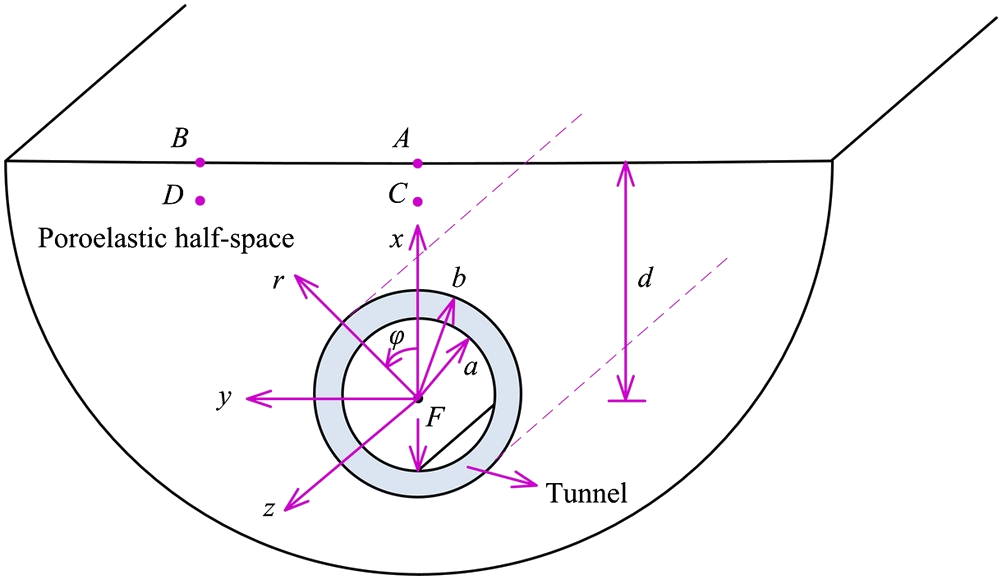
\includegraphics[width=0.85\textwidth]{figs/tunnel-halfspace.png}
	\end{figure}
\end{frame}

%------------------------------------------------
\begin{frame}
\frametitle{Geotechnical modeling of the complex world}
\begin{figure}
	\mode<beamer>{
		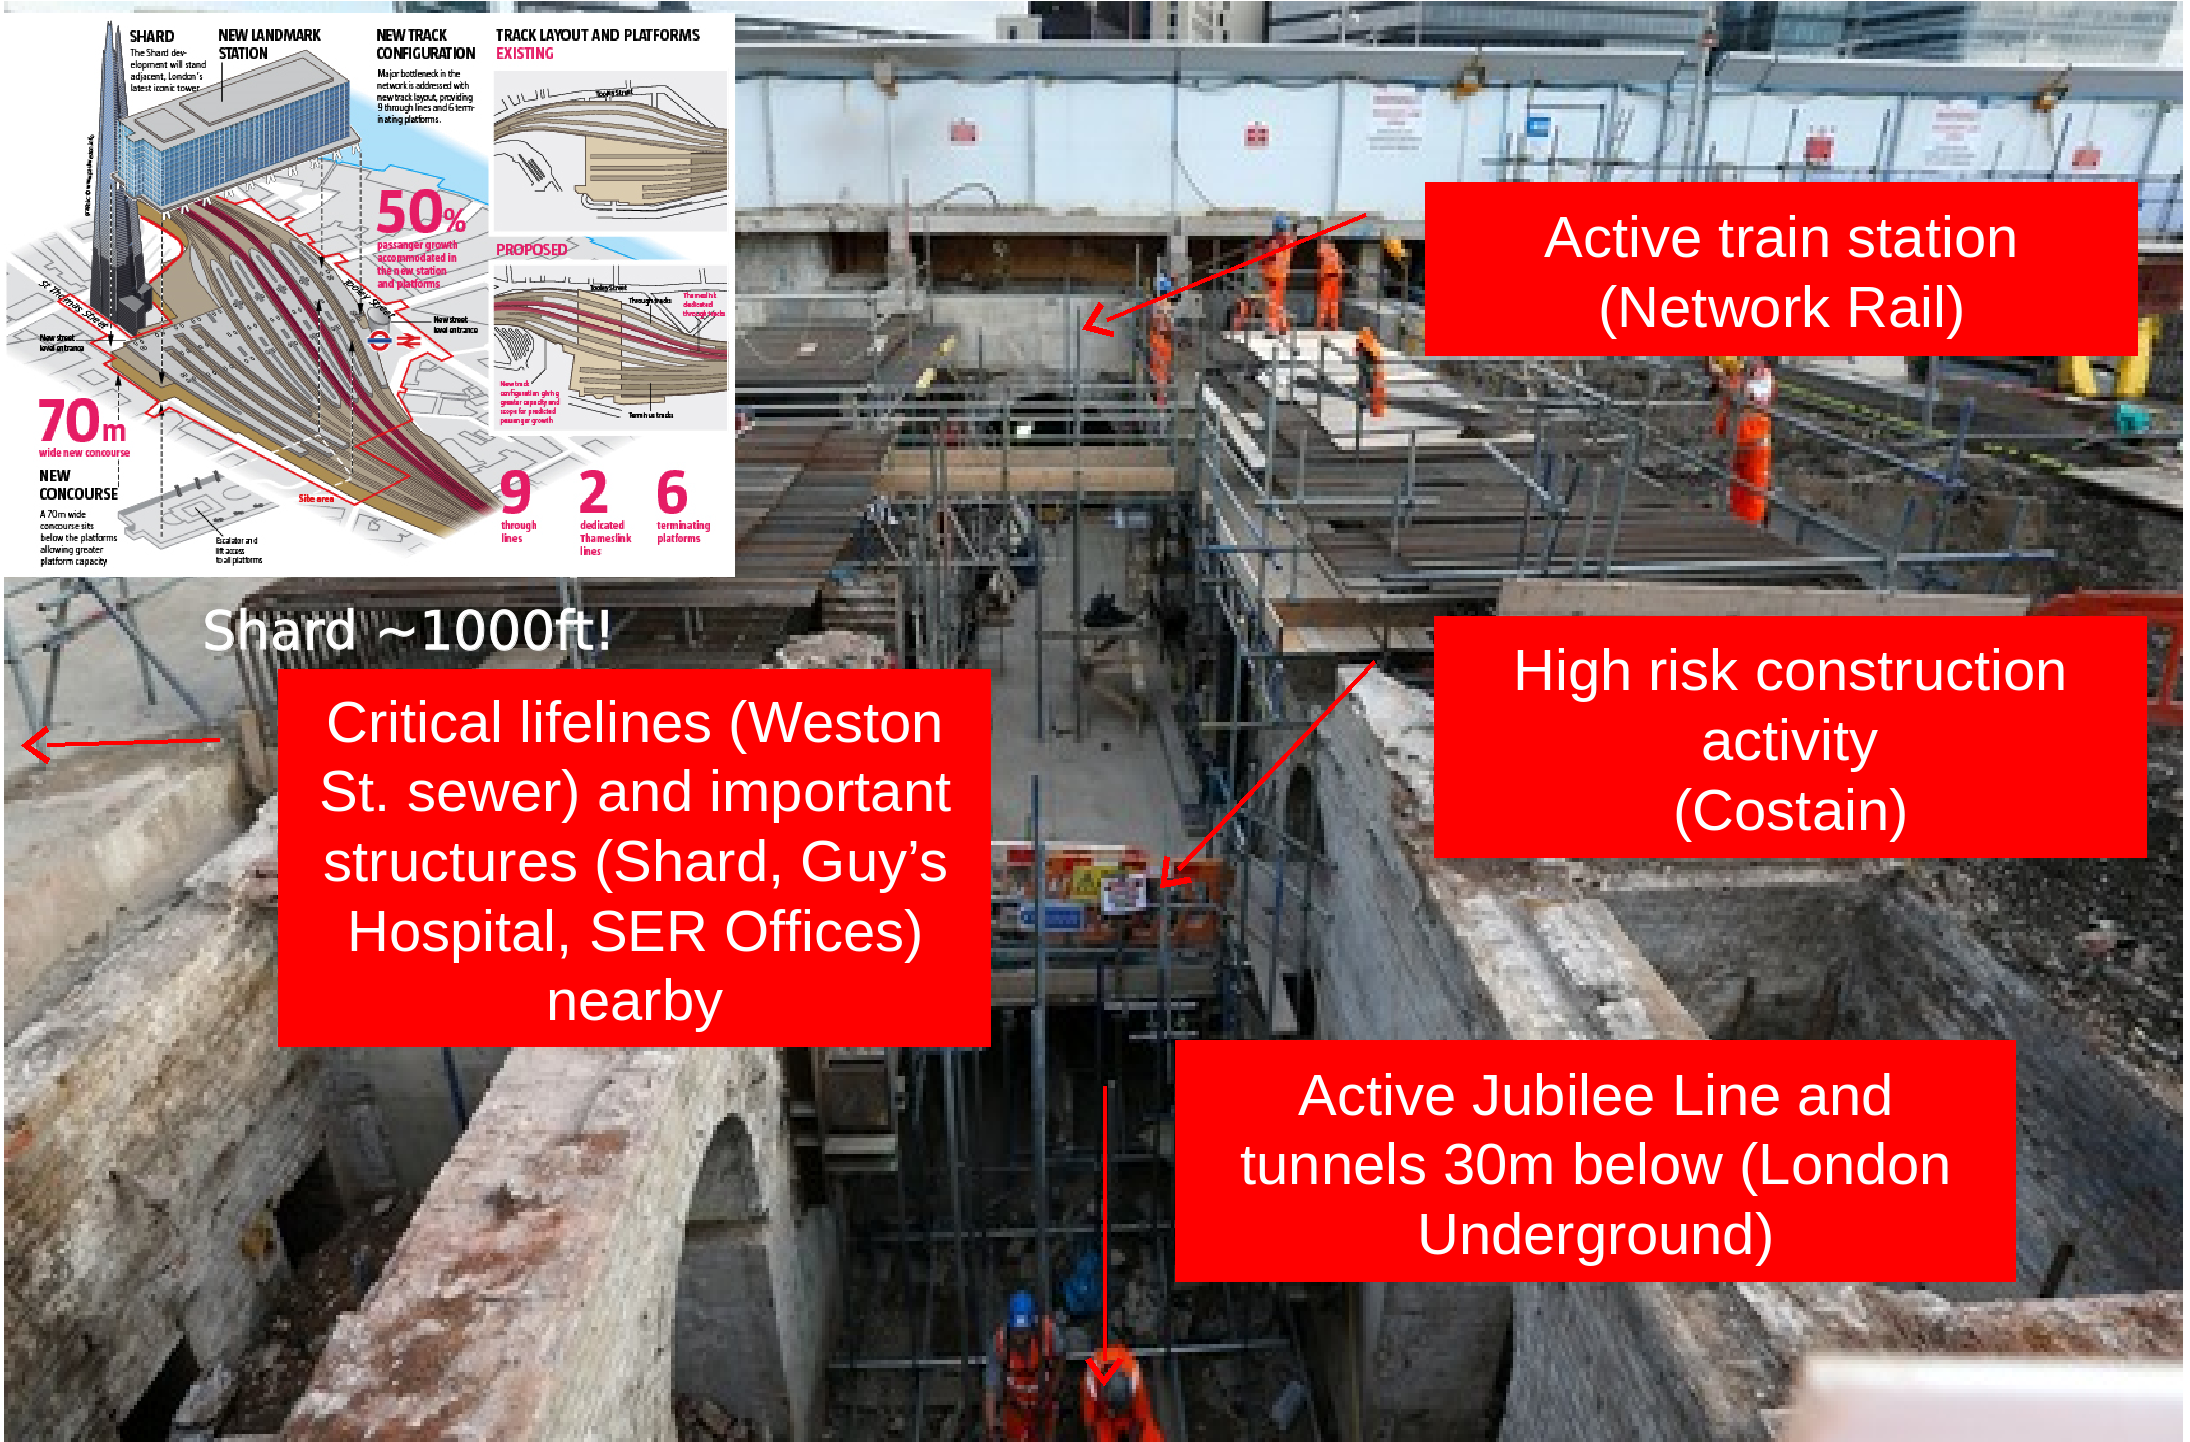
\includegraphics[width=0.85\textwidth]{figs/lbs.png}
	}
	\mode<handout>{
		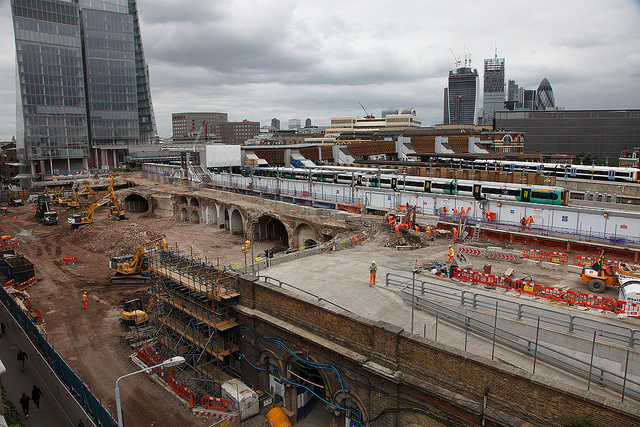
\includegraphics[width=0.85\textwidth]{figs/lbs-overview.jpg}
	}
	\caption*{London Bridge Station, London, UK}
\end{figure}
\end{frame}

%------------------------------------------------
\begin{frame}
\frametitle{Geotechnical modeling of the complex world}
\begin{figure}
	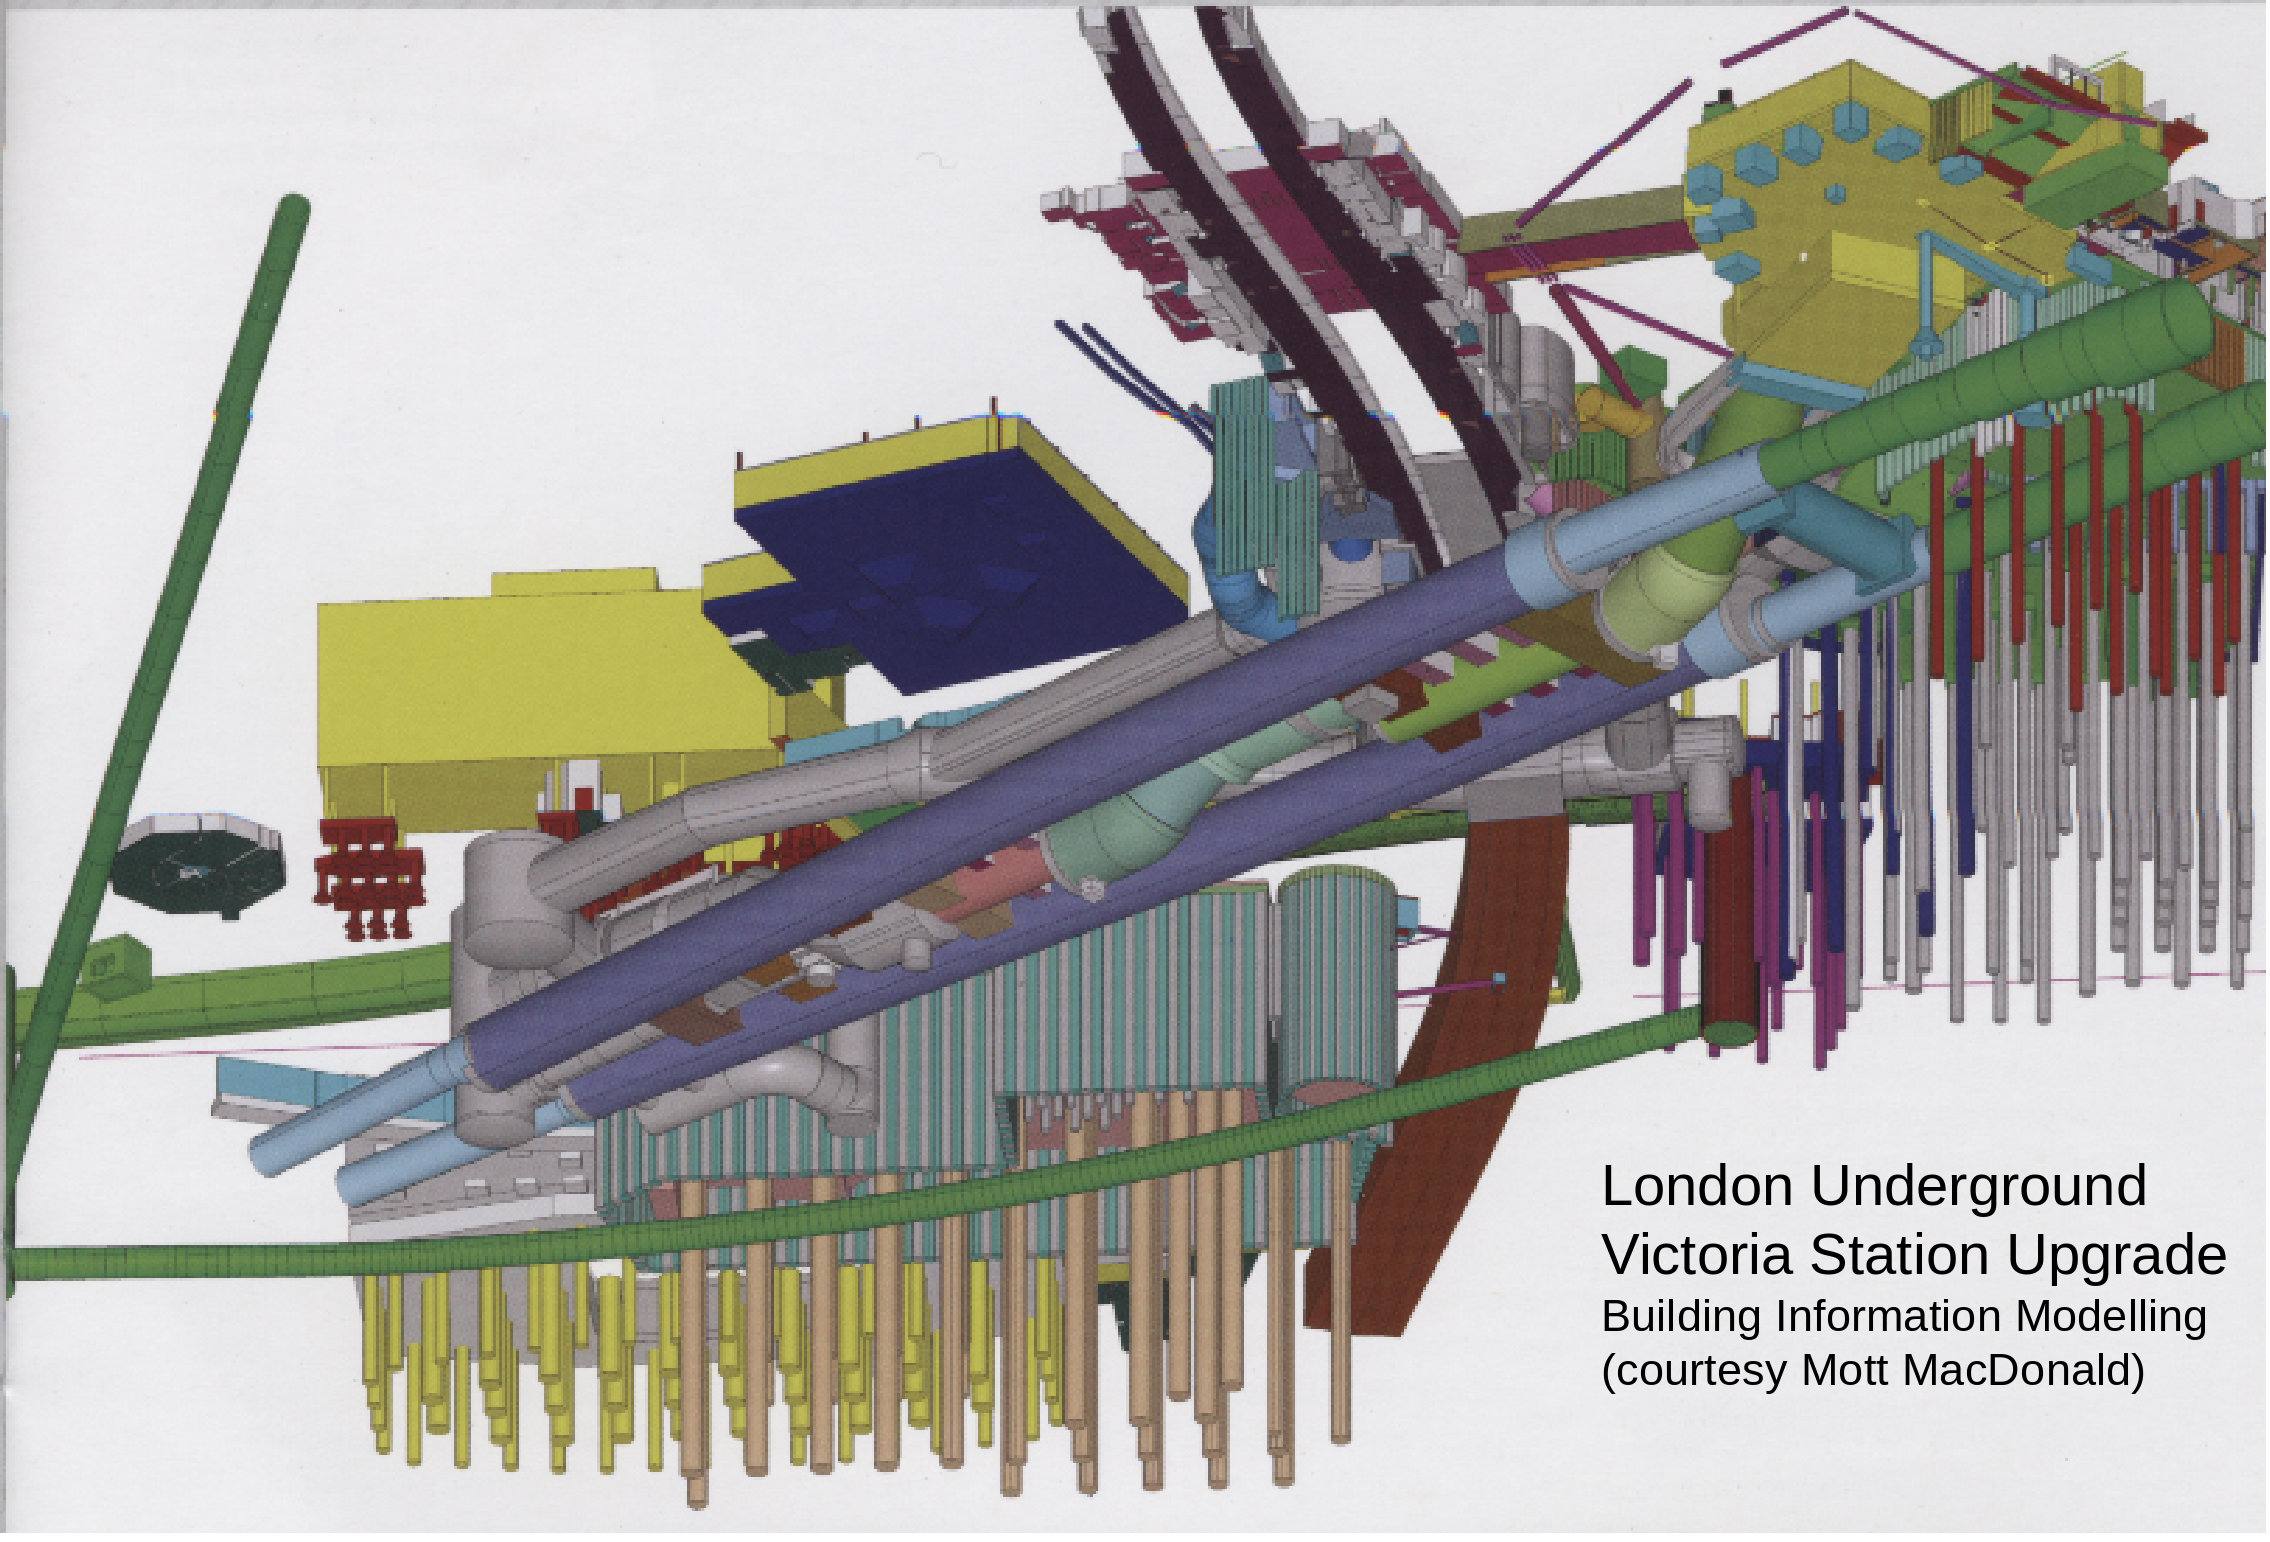
\includegraphics[width=0.85\textwidth]{figs/victoria-station.png}
	\caption{London Victoria station upgrade, London, UK}
\end{figure}
\end{frame}

\note{Movements must be estimated, both of the structure and of the ground. 
	This is particularly important if there are adjacent buildings and for 
	sensitive services. For example, if an excavation is to be made in an 
	urban area close to existing services and buildings, one of the key 
	design constraints is the effect that the excavation has on the adjacent 
	structures and services. It may be necessary to predict any structural 
	forces induced in these existing structures and/or services.}


%------------------------------------------------
\begin{frame}
	\frametitle{Local vs global stability}
	\begin{figure}
		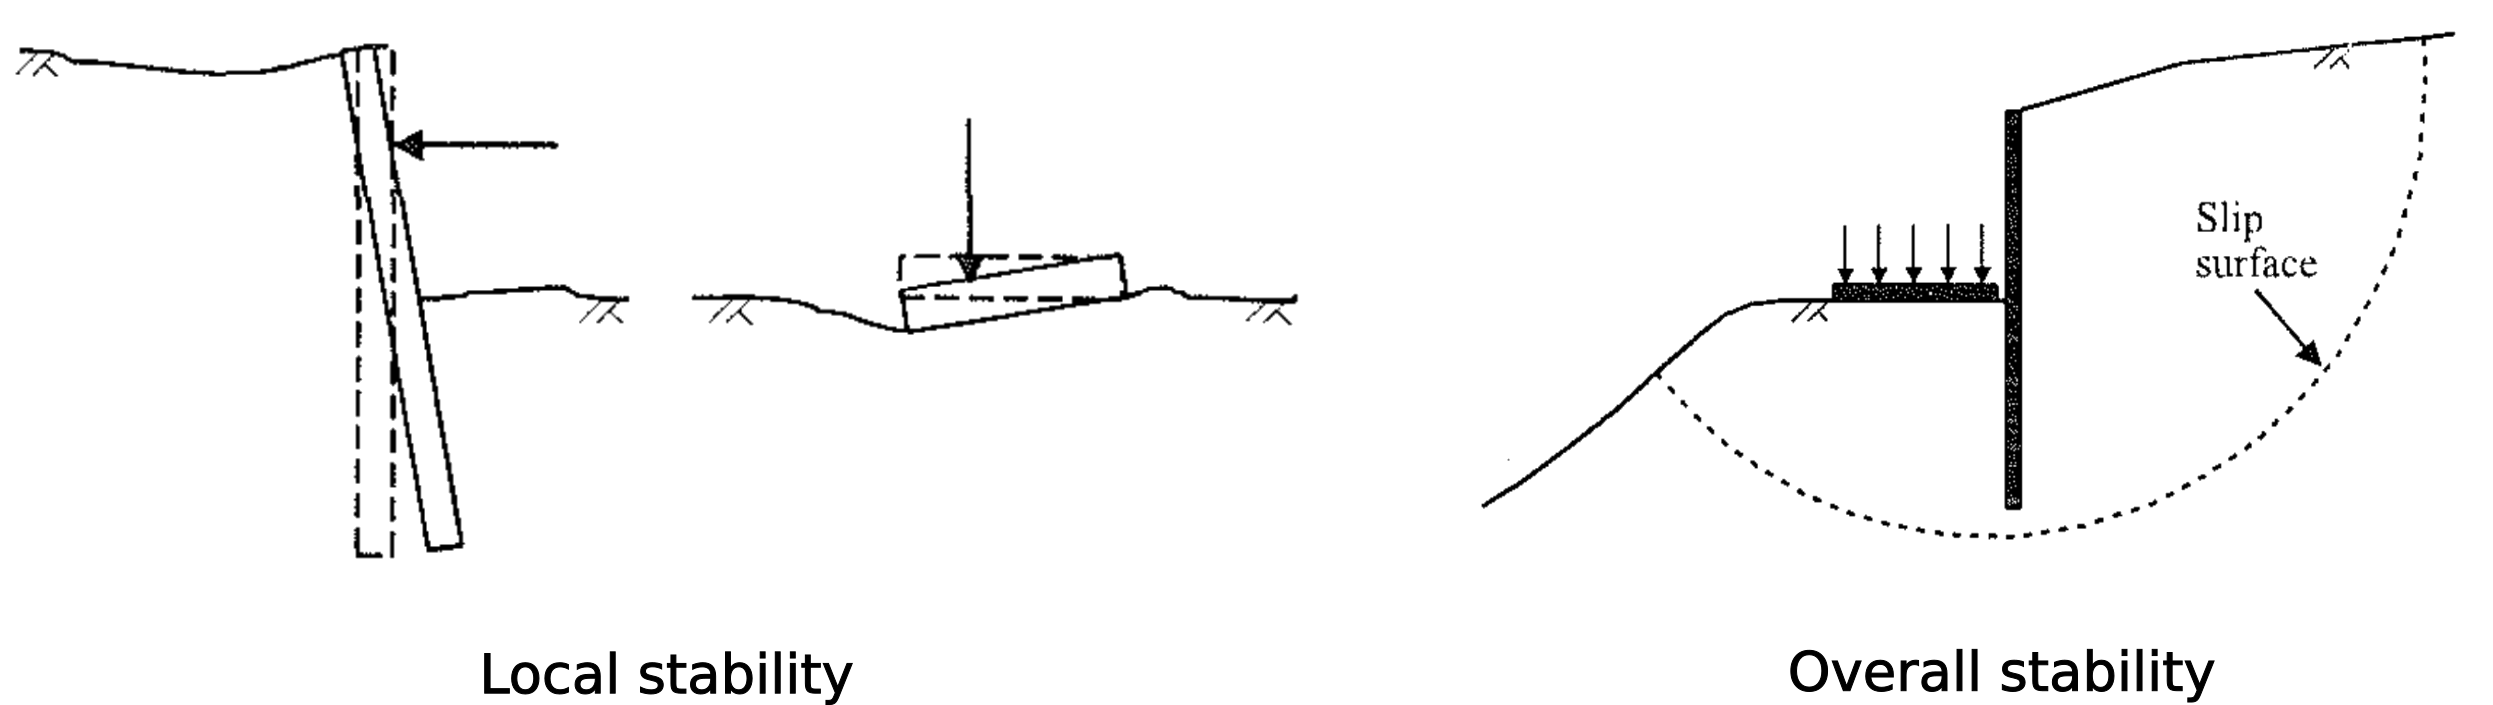
\includegraphics[width=0.95\textwidth]{figs/stability.png}
	\end{figure}
\end{frame}
\note{When designing any geotechnical structure, the engineer must ensure that it is
	stable. Stability can take several forms. Firstly, the structure and support 
	system must be stable as a whole. There must be no danger of rotational, 
	vertical or translational failure (\textbf{\textit{local stability}}). 
	Secondly, \textbf{\textit{overall stability}} must be established. For example, 
	if a retaining 	structure supports sloping ground, the possibility of the 
	construction promoting an overall slope failure should be investigated.
}

%------------------------------------------------
\begin{frame}
\frametitle{Geotechnical modeling}
\begin{figure}
  \mode<beamer>{
	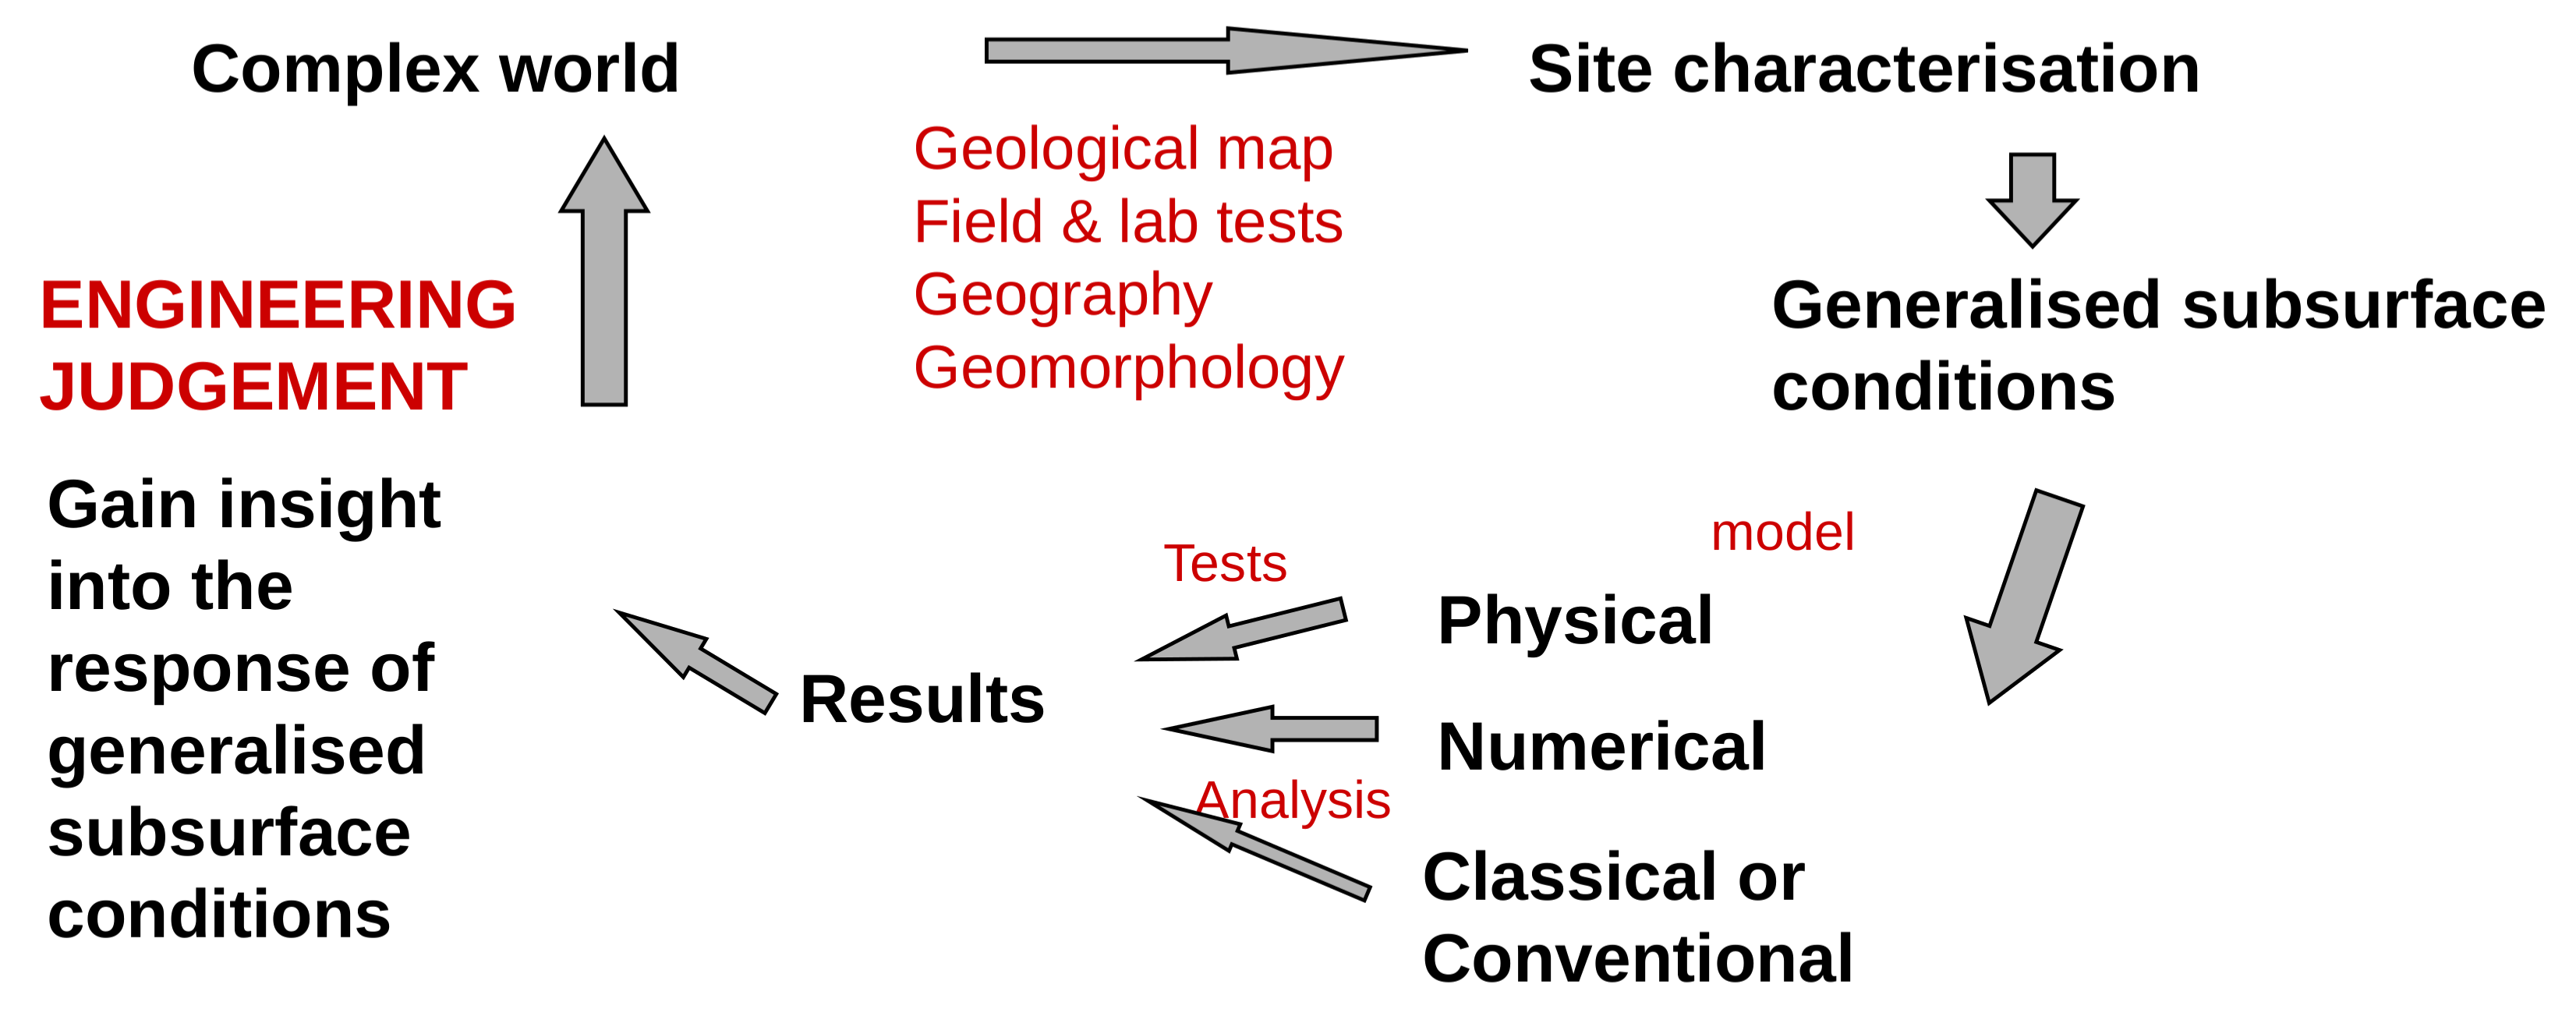
\includegraphics[width=0.95\textwidth]{figs/geotechnical-modeling-final.png}
  }
  \mode<handout>{
	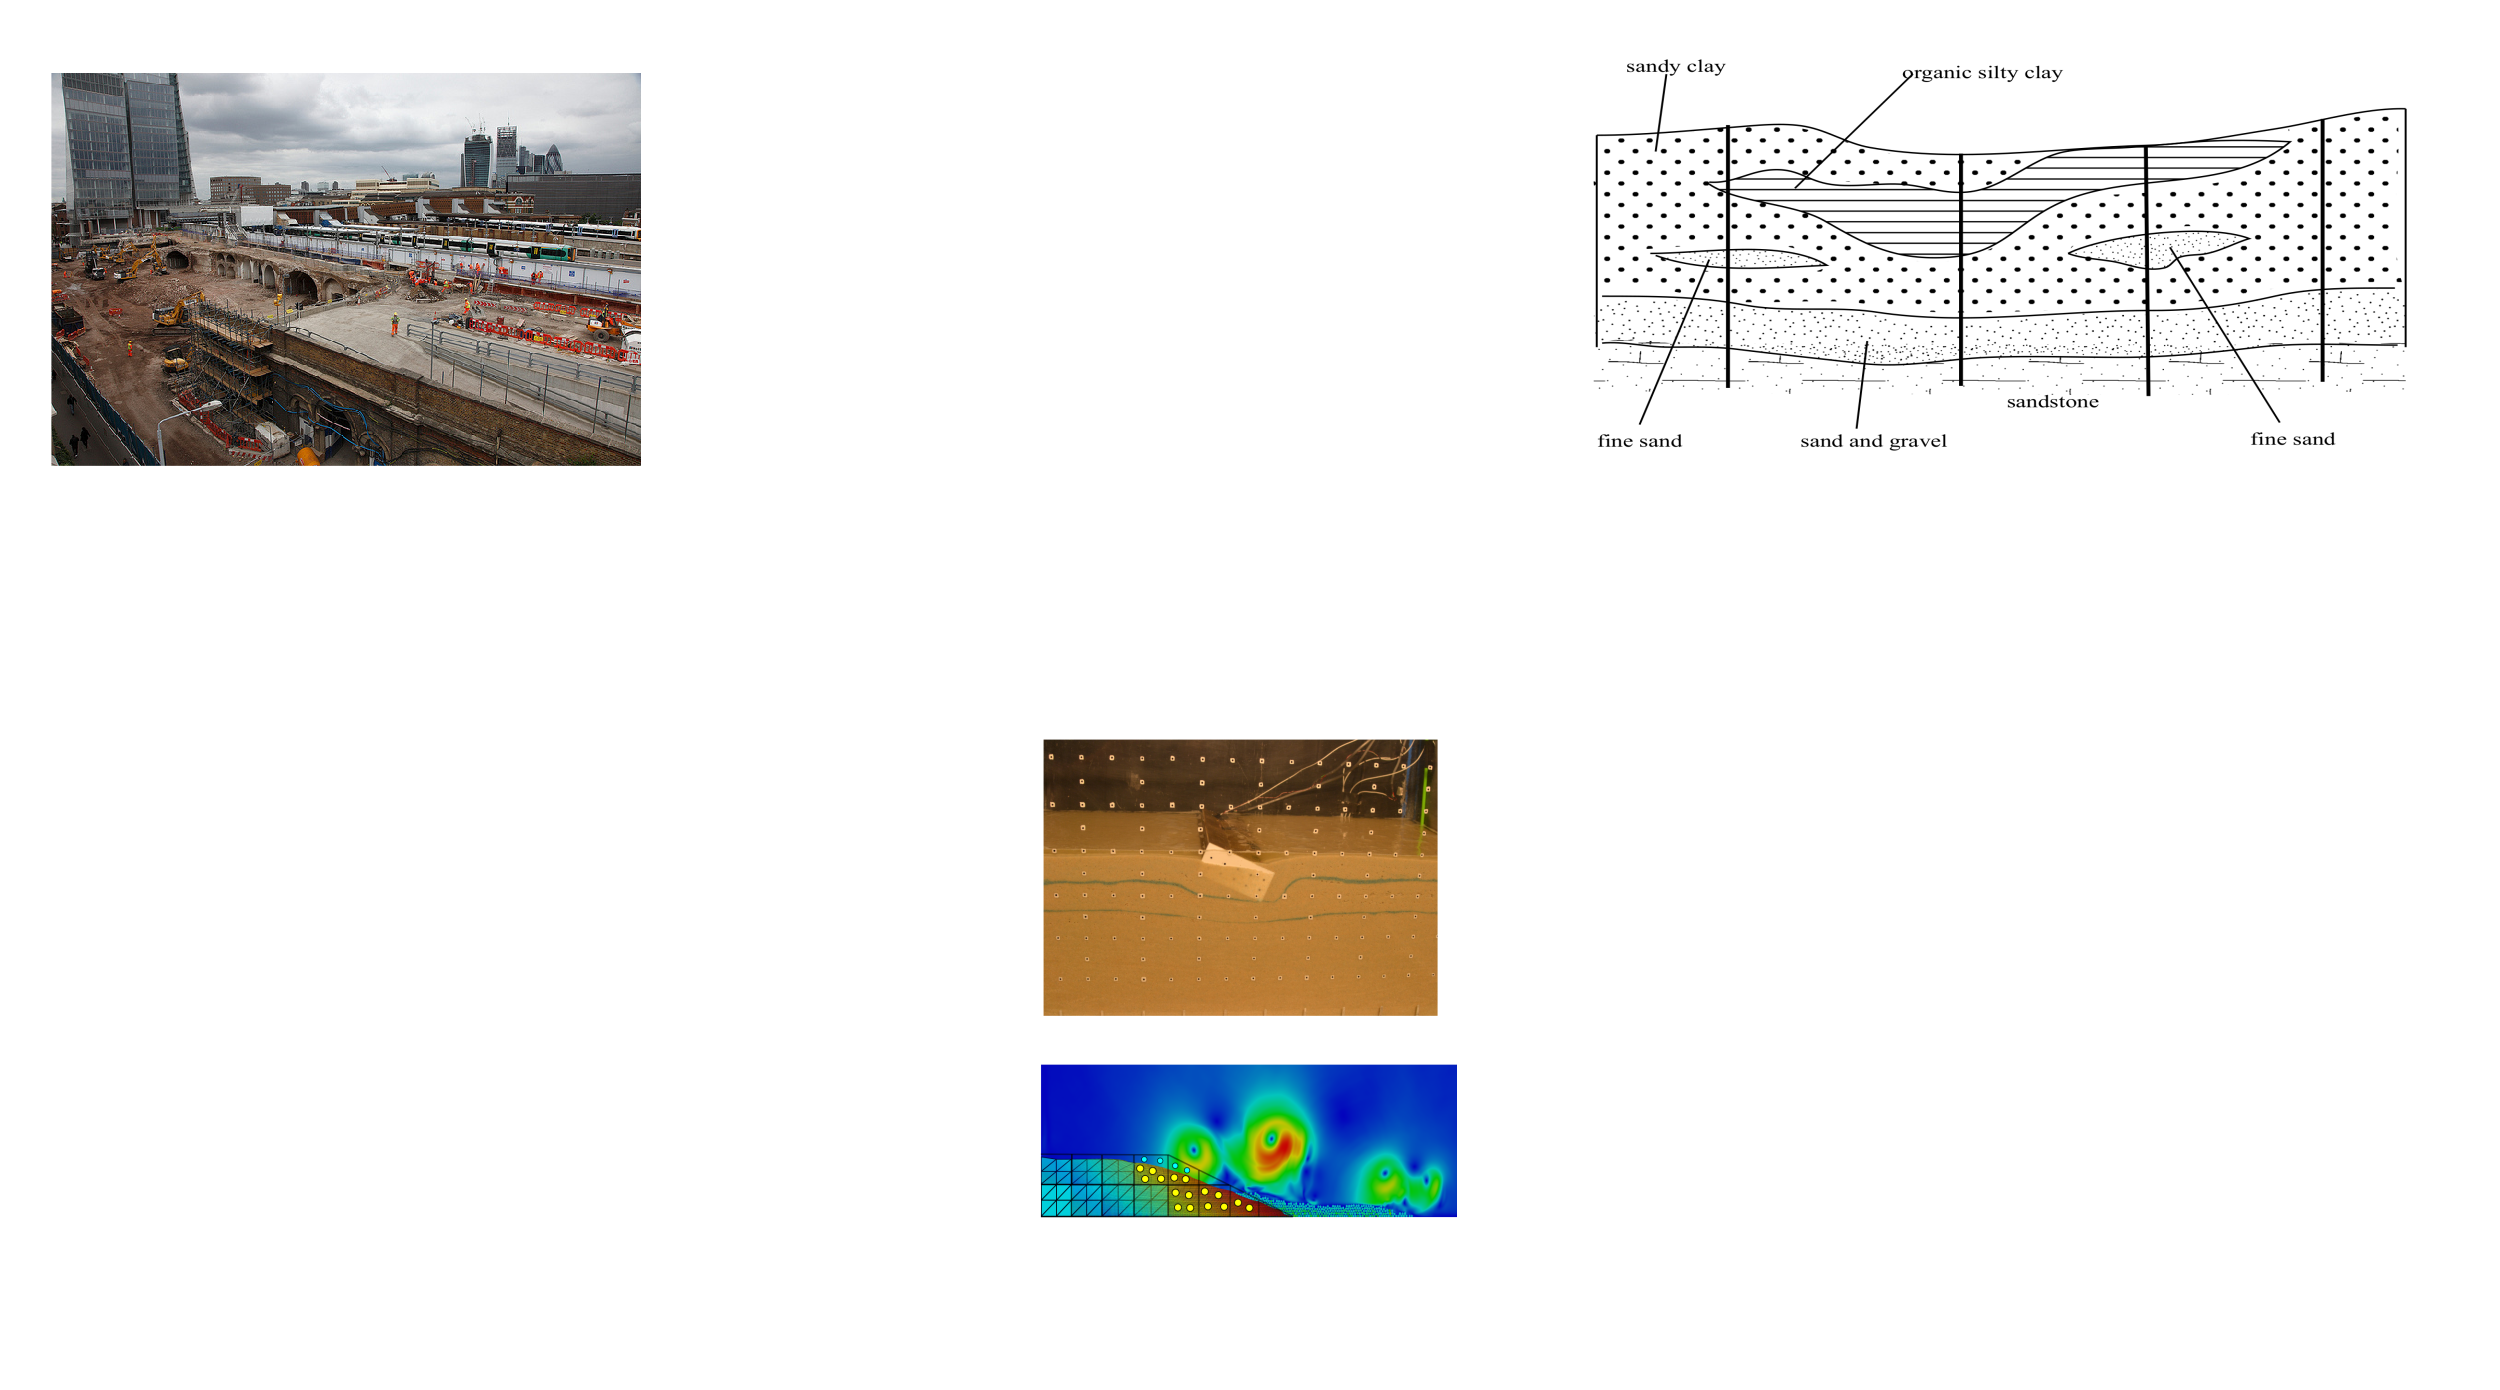
\includegraphics[width=0.95\textwidth]{figs/geotechnical-modeling.png}
  }
\end{figure}
\end{frame}

\note{\textbf{Design requirements:} Before the design process can begin, a considerable 
	amount of information must
	be assembled. The basic geometry and loading conditions must be established.
	These are usually defined by the nature of the engineering project.\\
	
	A geotechnical site investigation is then required to establish the ground
	conditions. Both the soil stratigraphy and soil properties should be determined. In
	this respect it will be necessary to determine the strength of the soil and, if ground
	movements are important, to evaluate its stiffness too. The position of the ground
	water table and whether or not there is underdrainage or artesian conditions must
	also be established. The possibility of any changes to these water conditions should
	be investigated. For example, in many major cities around the world the ground
	water level is rising.}

\note{The site investigation should also establish the location of any services (gas,
	water, electricity, telecommunications, sewers andlor tunnels) that are in the
	vicinity of the proposed construction. The type (strip, raft andlor piled) and depth
	of the foundations of any adjacent buildings should also be determined. The
	allowable movements of these services and foundations should then be established.\\
	Any restrictions on the performance of the new geotechnical structure must be
	identified. Such restrictions can take many different forms. For example, due to the
	close proximity of adjacent services and structures there may be restrictions
	imposed on ground movements.}

\note{Once the above information has been collected, the design constraints on the
	geotechnical structure can be established. These should cover the construction
	period and the design life of the structure. This process also implicitly identifies
	which types of structure are and are not appropriate. For example, when designing
	an excavation, if there is a restriction on the movement of the retained ground,
	propped or anchored embedded retaining walls are likely to be more appropriate
	than gravity or reinforced earth walls. The design constraints also determine the
	type of design analysis that needs to be undertaken.}

%------------------------------------------------
\begin{frame}
\frametitle{Geotechnical modeling: What should be modeled?}
\mode<beamer>{
\begin{itemize}
	\item Self weight effect of soils (This is why soil moves)
	\item Construction sequence (Complex geometry)
	\item Water movement (undrained, consolidation, drained)
	\item Insitu stresses (stiffness/strength depends on current stresses and stress history)
	\item Predict the ability of a design to withstand extreme loading conditions (you only have one chance)
\end{itemize}
}
\mode<handout>{
\vspace{4cm}
}
\begin{figure}
	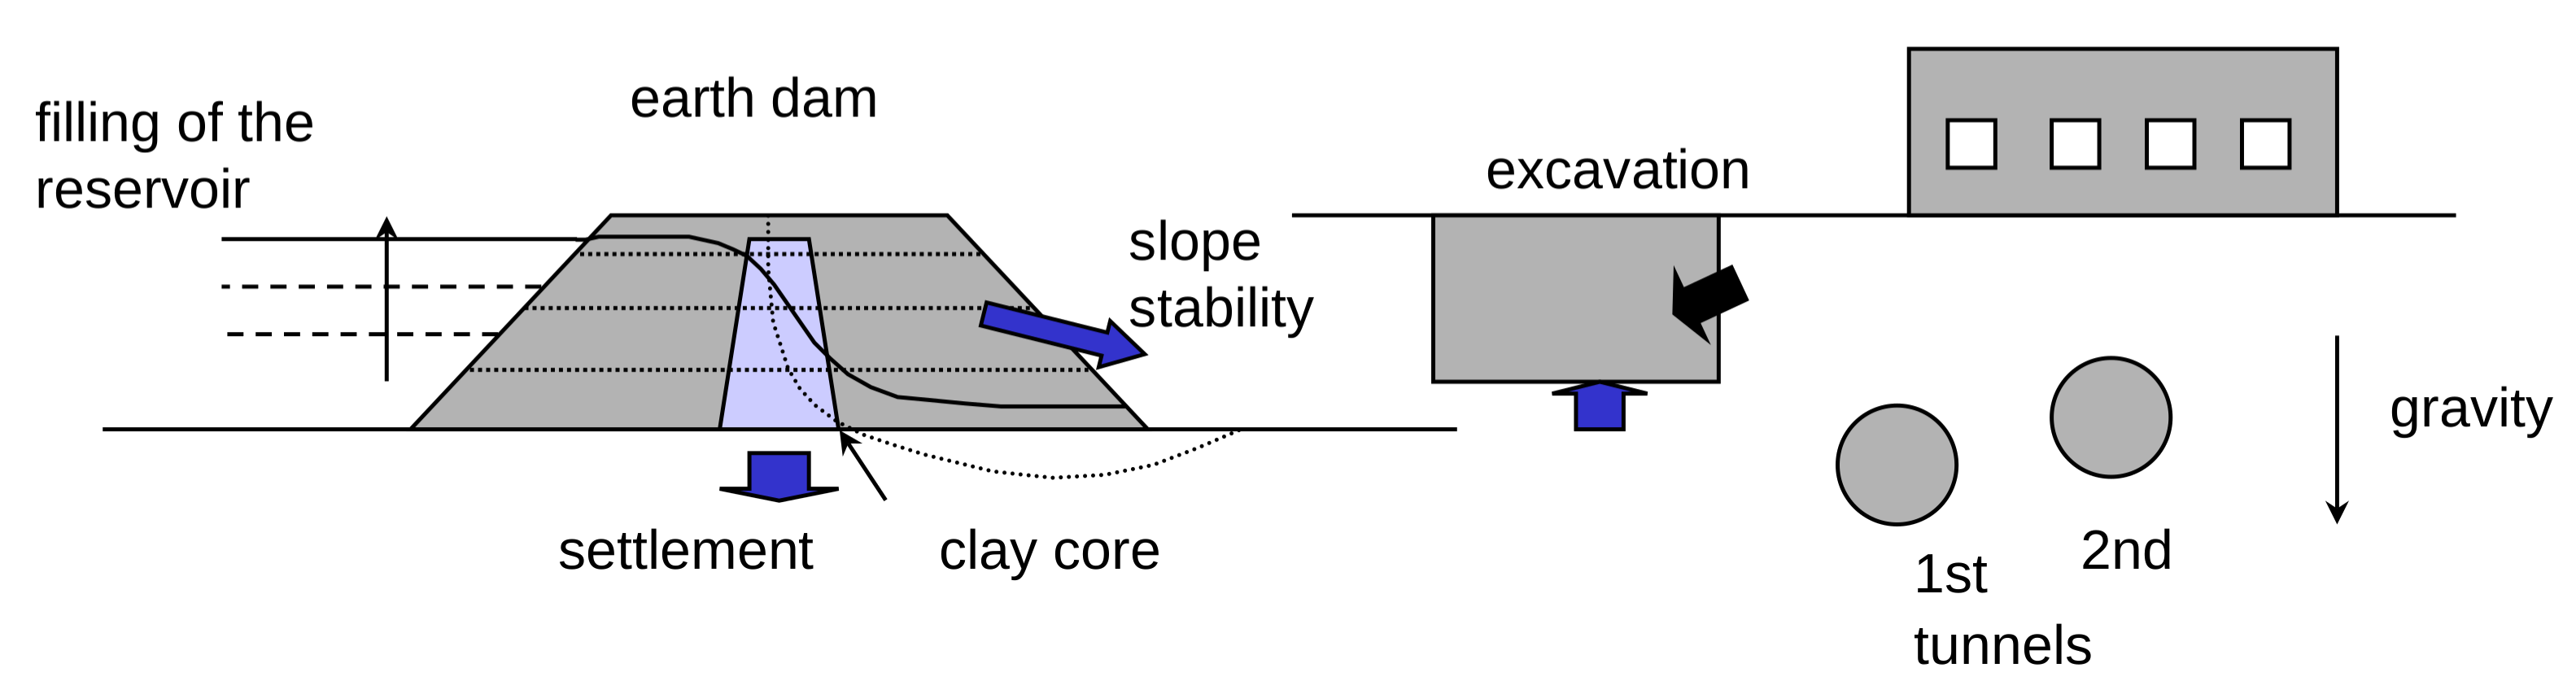
\includegraphics[width=0.95\textwidth]{figs/geotechnical-modeling-examples.png}
\end{figure}
\end{frame}

%------------------------------------------------
\begin{frame}
\frametitle{Scales of modeling in geotechnical engineering}
	\begin{figure}
		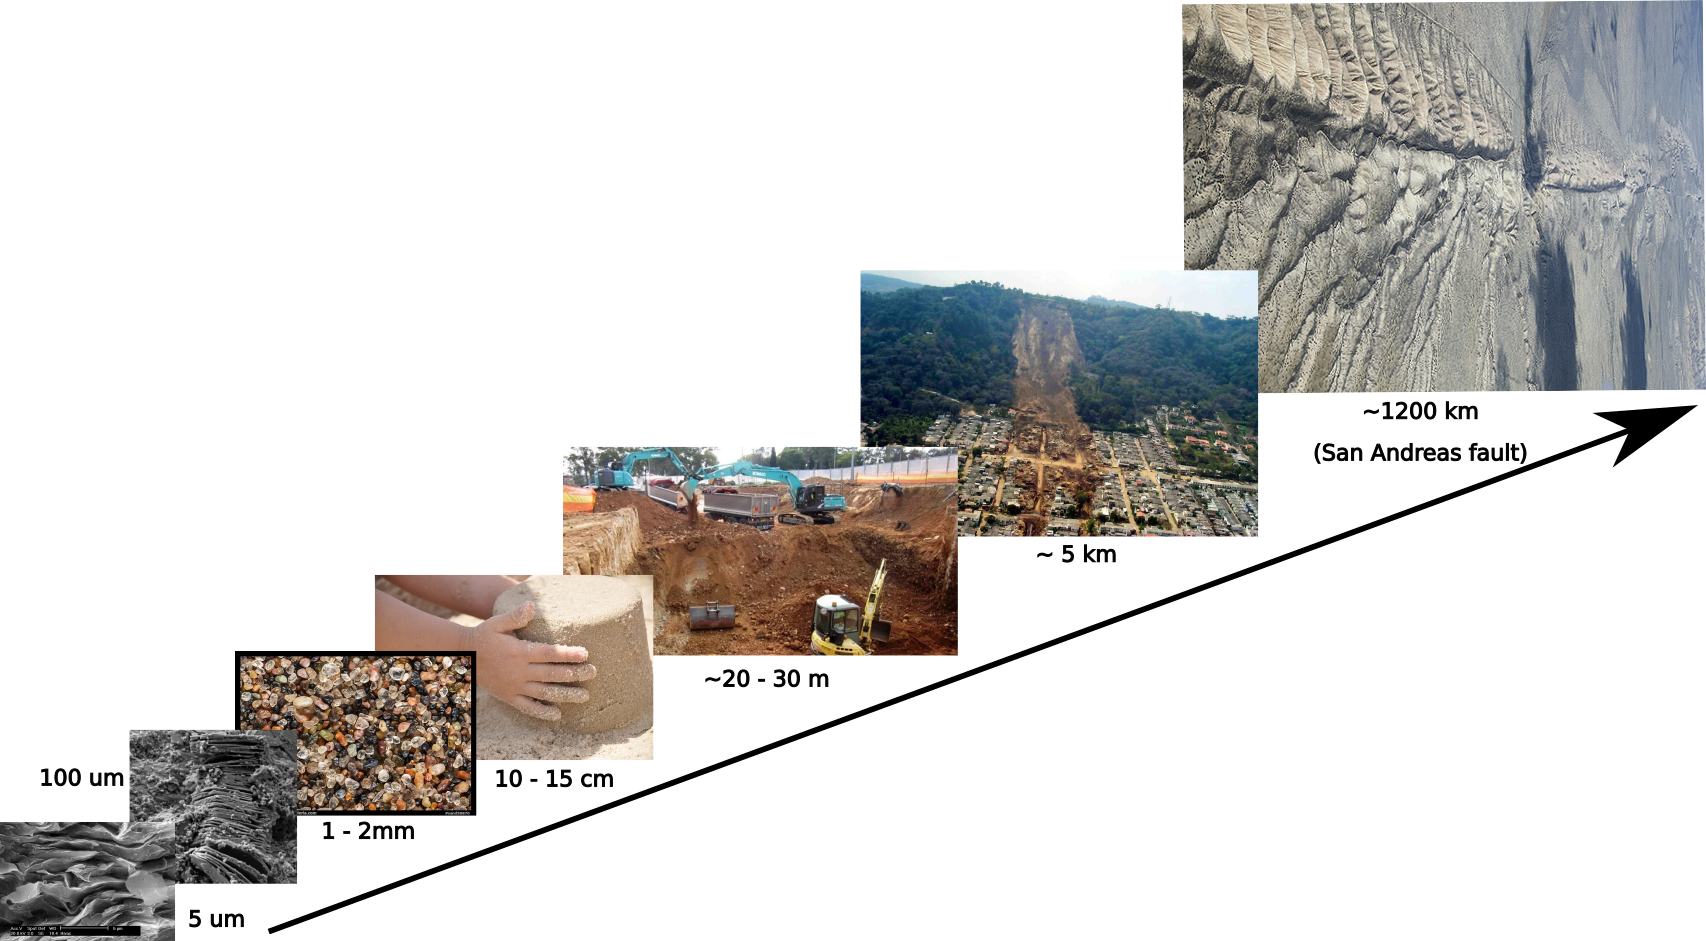
\includegraphics[width=0.95\textwidth]{figs/soil-scale.png}
	\end{figure}
\end{frame}

%------------------------------------------------
\begin{frame}
\frametitle{Soil behavior}
\mode<beamer>{
\begin{itemize}
	\item nonhomogeneous,
	\item anisotropic, 
	\item non-linear, 
	\item initial stress conditions, 
	\item stress history
	\item Geometry - very complex
\end{itemize}
\textbf{Soil Mechanics in practice - largely empirical}
}
\end{frame}

\subsection{Oso landslide}
%------------------------------------------------
\begin{frame}
	\frametitle{Oso landslide: case study}
	\begin{figure}
		\includegraphics[width=0.9\textwidth]{figs/oso/oso-slide.png}
	\end{figure}
\end{frame}

%------------------------------------------------
\begin{frame}
	\frametitle{Oso landslide: case study}
	\begin{figure}
		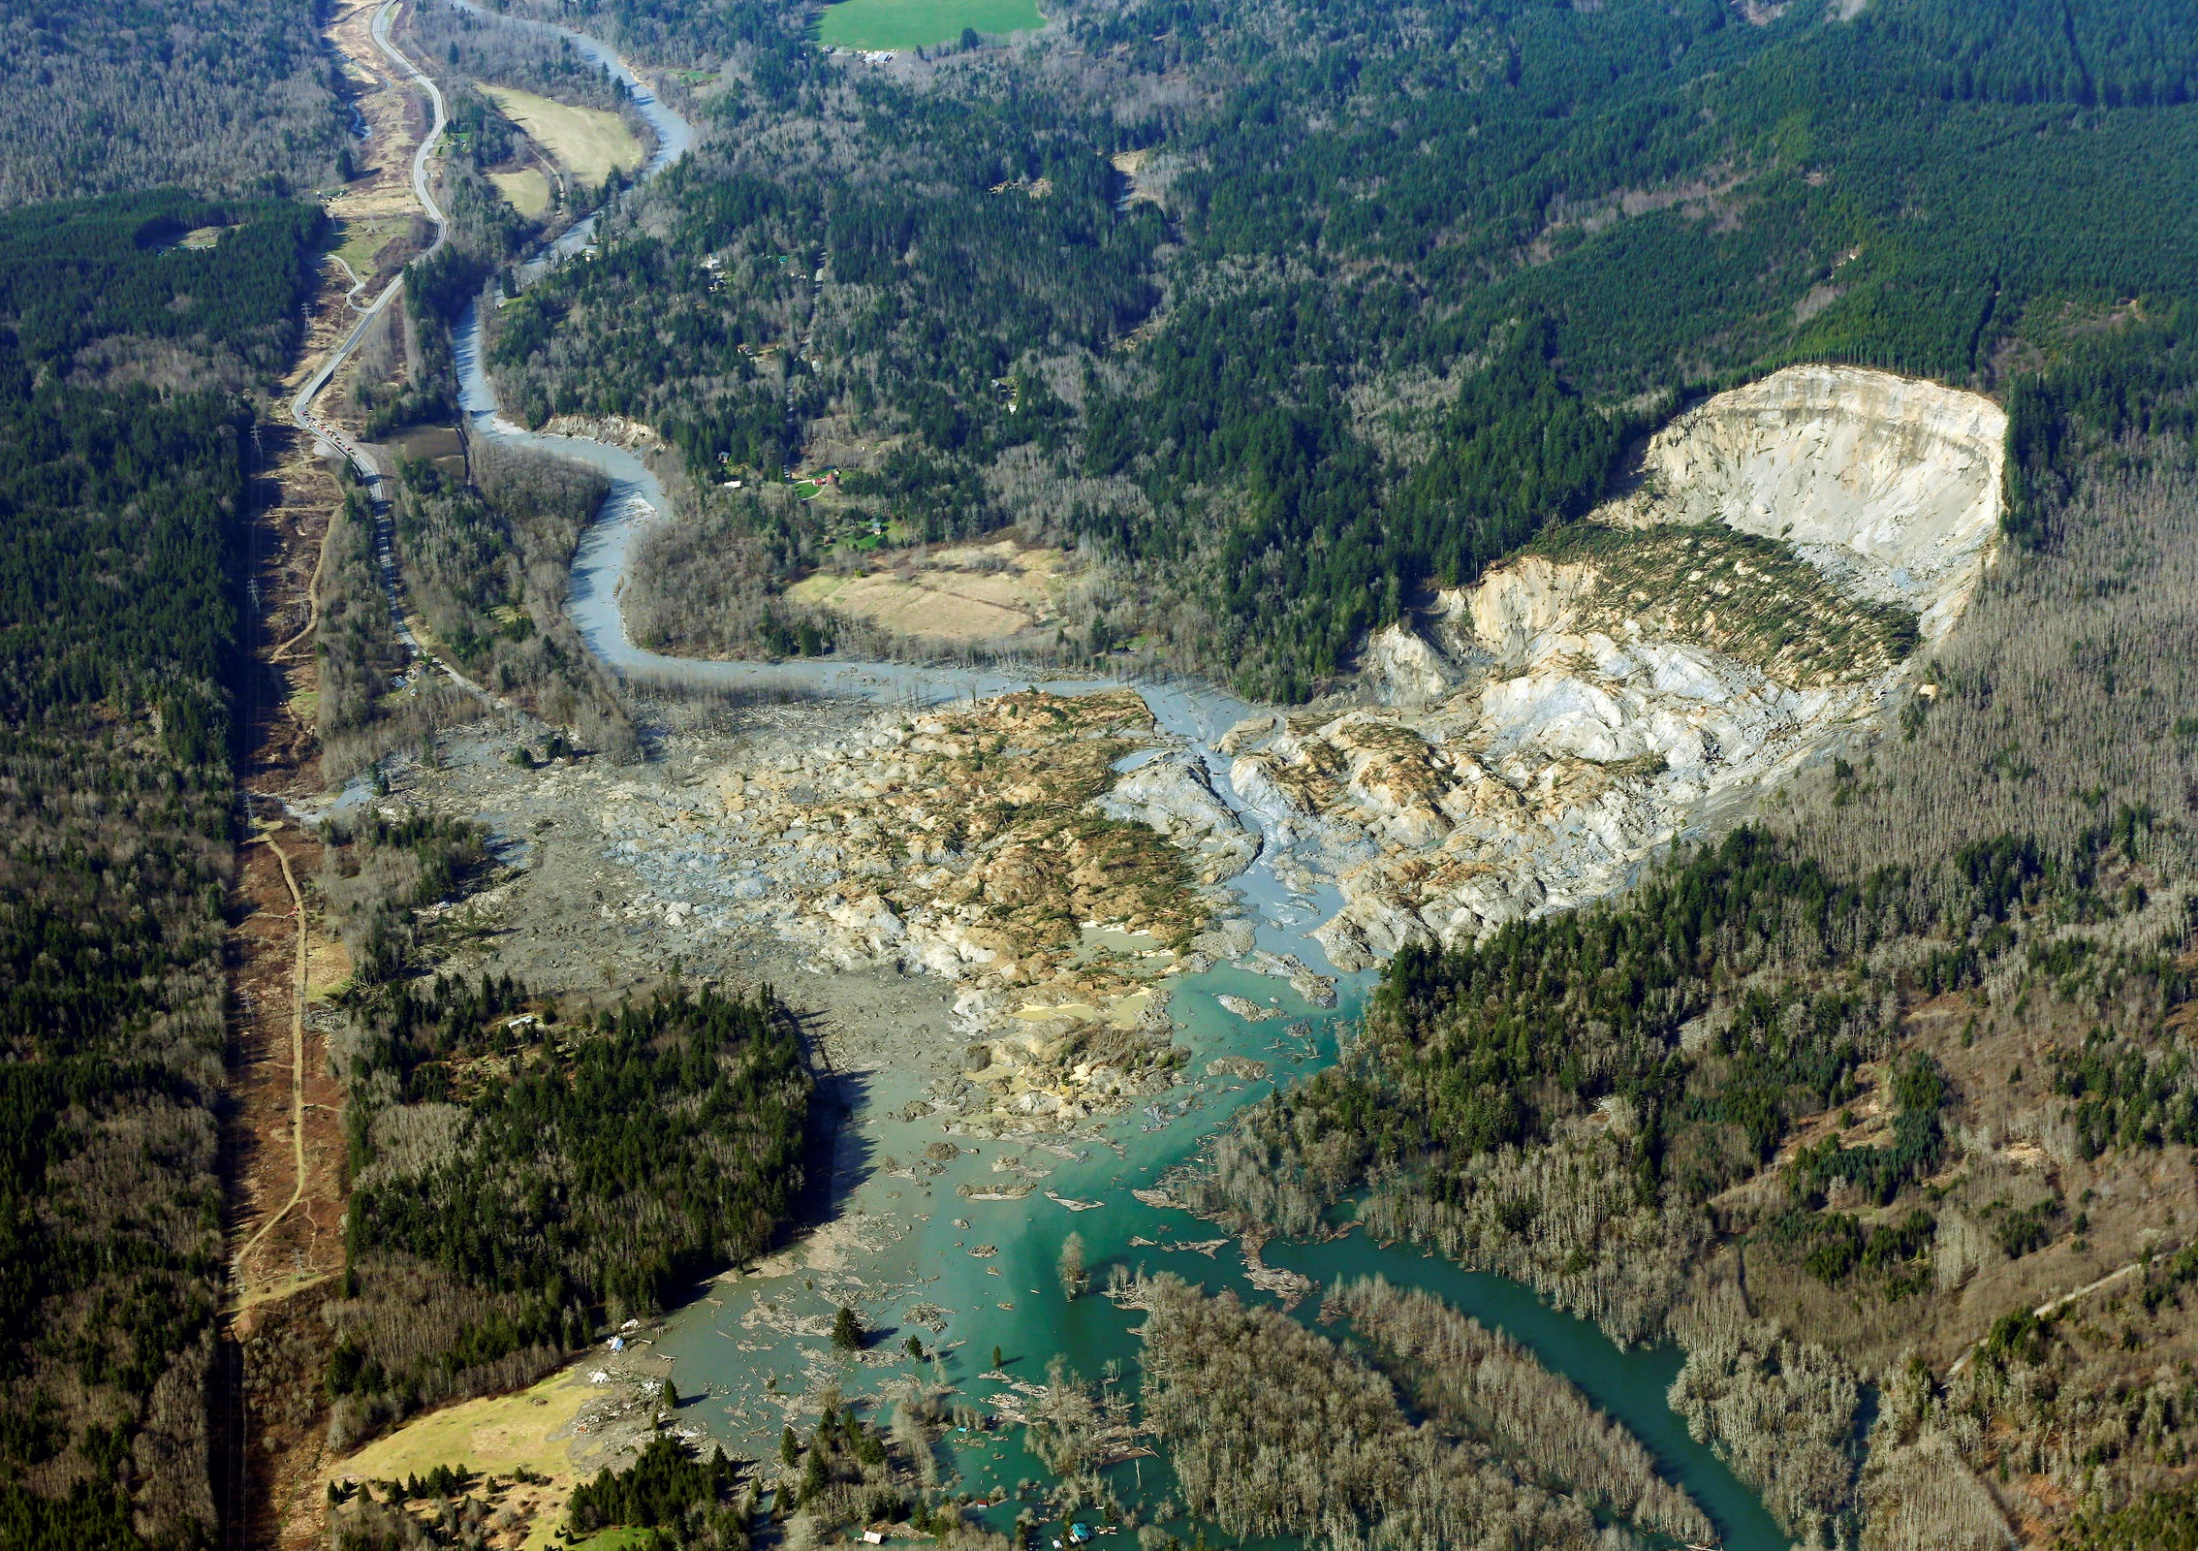
\includegraphics[width=0.9\textwidth]{figs/oso/oso-slide1.jpeg}
	\end{figure}
\end{frame}

\note{
\begin{itemize}
	\item 22nd March 2014 at 10:37 AM
	\item Volume approx 8 million cubic meters
	\item 43 casualties (deadliest landslide in the US)
	\item 1 neighborhood destroyed
	\item (unknown but) $>$ 150 million lost cost (DNR 2015), 
	+ USD 65 million (lawsuit 2017) + indirect costs
	\item Social tensions and Indian Snohomish tribe
\end{itemize}
}


%------------------------------------------------
\begin{frame}
	\frametitle{Oso landslide: topography}
	\begin{figure}
		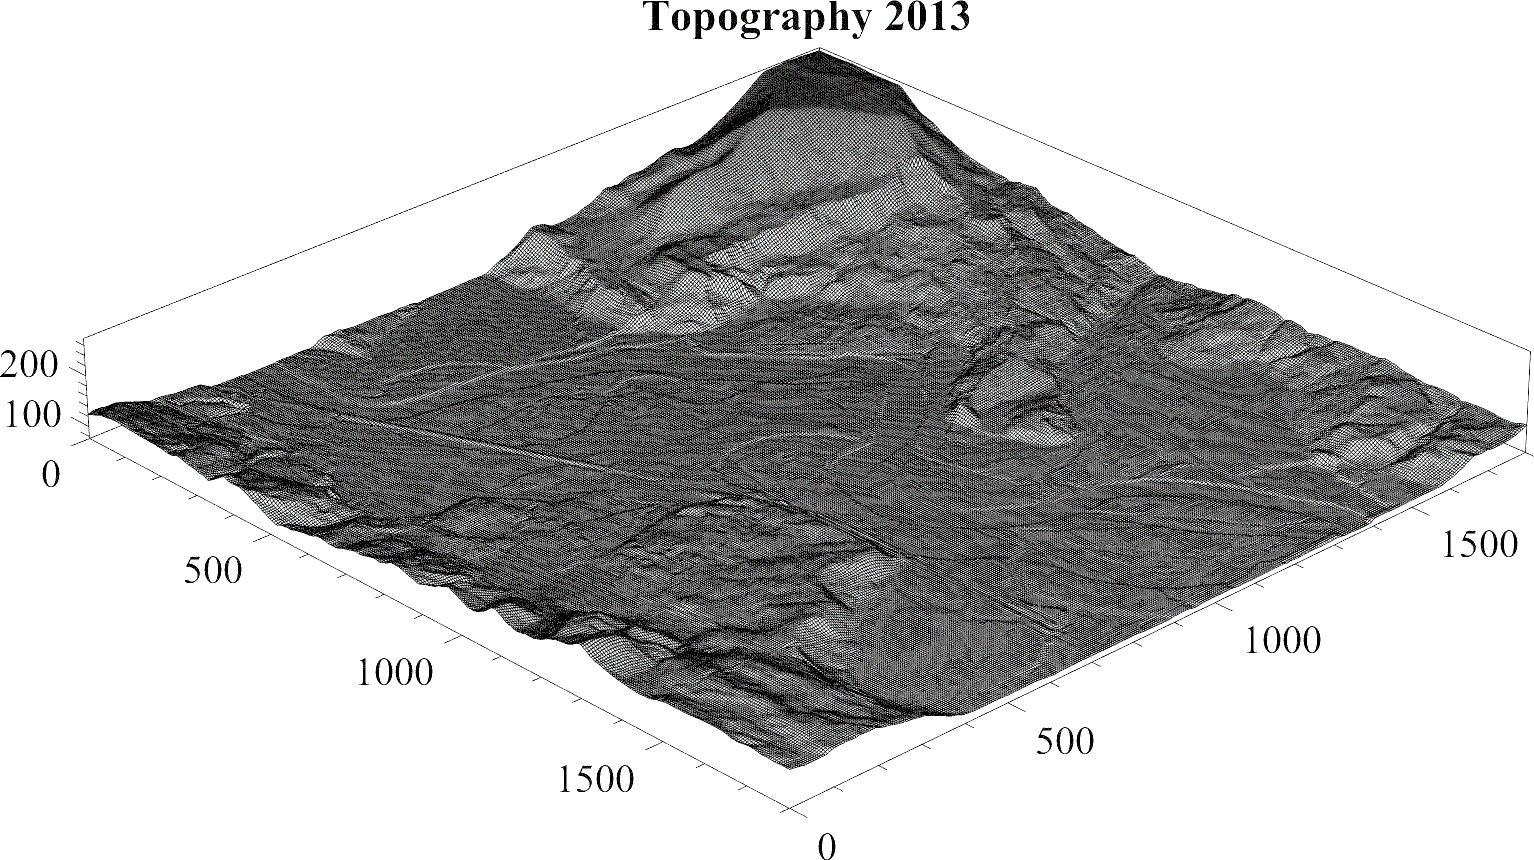
\includegraphics[width=0.95\textwidth]{figs/oso/topography-2013.png}
	\end{figure}
\end{frame}

%------------------------------------------------
\begin{frame}
	\frametitle{Oso landslide: topography}
	\begin{figure}
		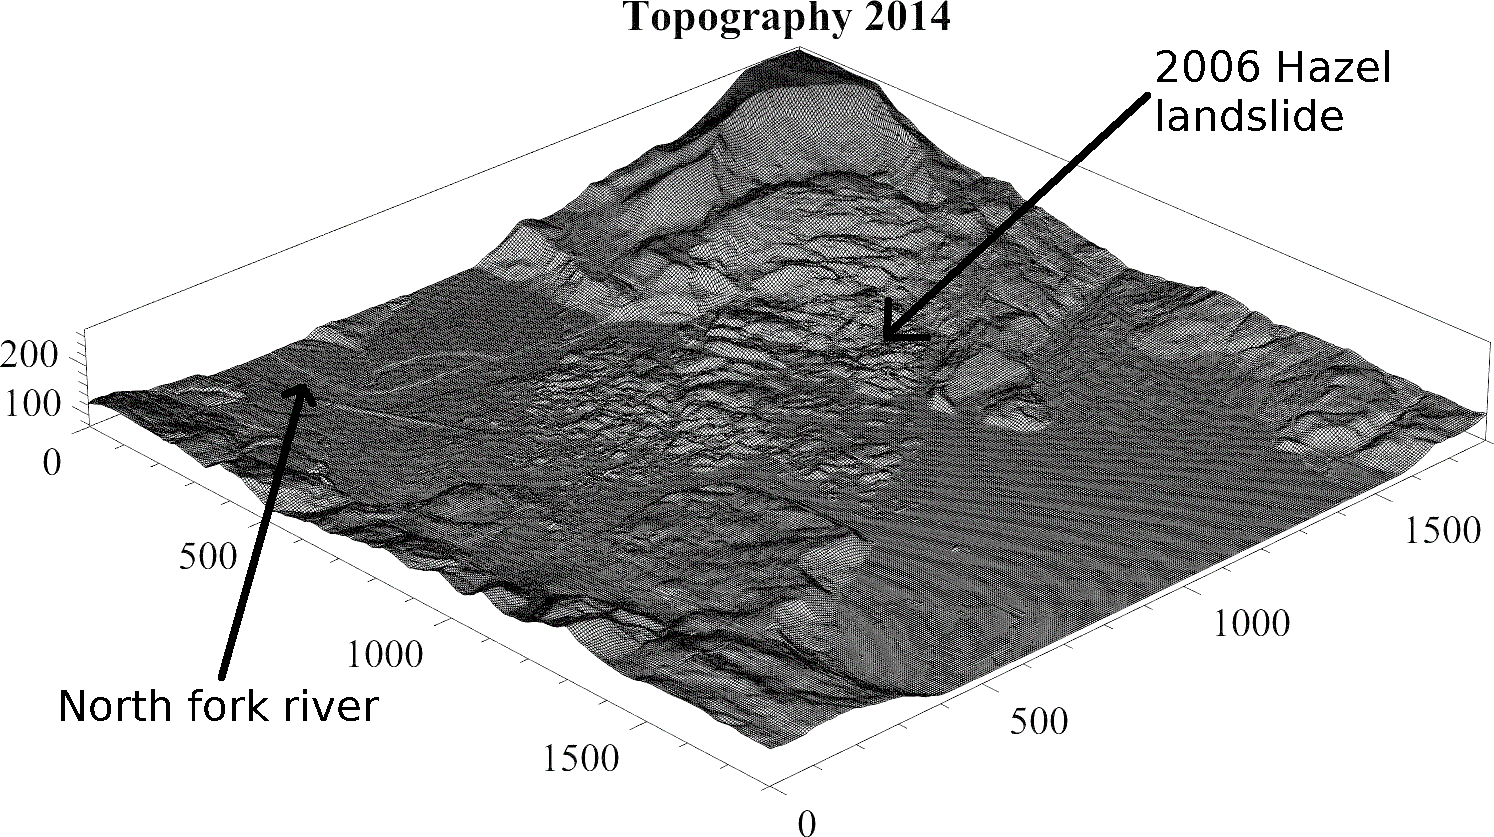
\includegraphics[width=0.95\textwidth]{figs/oso/topography-2014.png}
	\end{figure}
\end{frame}

%------------------------------------------------
\begin{frame}
	\frametitle{Oso landslide: historic slides}
	\begin{figure}
		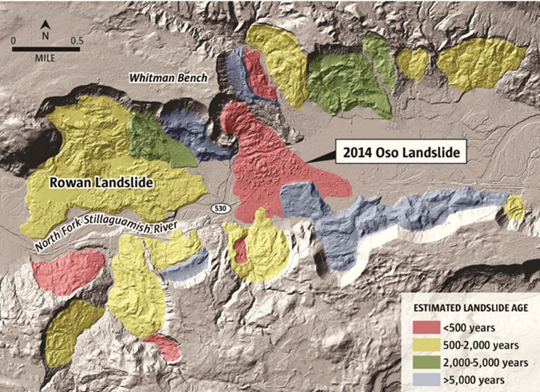
\includegraphics[width=0.9\textwidth]{figs/oso/past-slides.png}
	\end{figure}
\end{frame}

%------------------------------------------------
\begin{frame}
	\frametitle{Oso landslide: Soil profile}
	\begin{figure}
		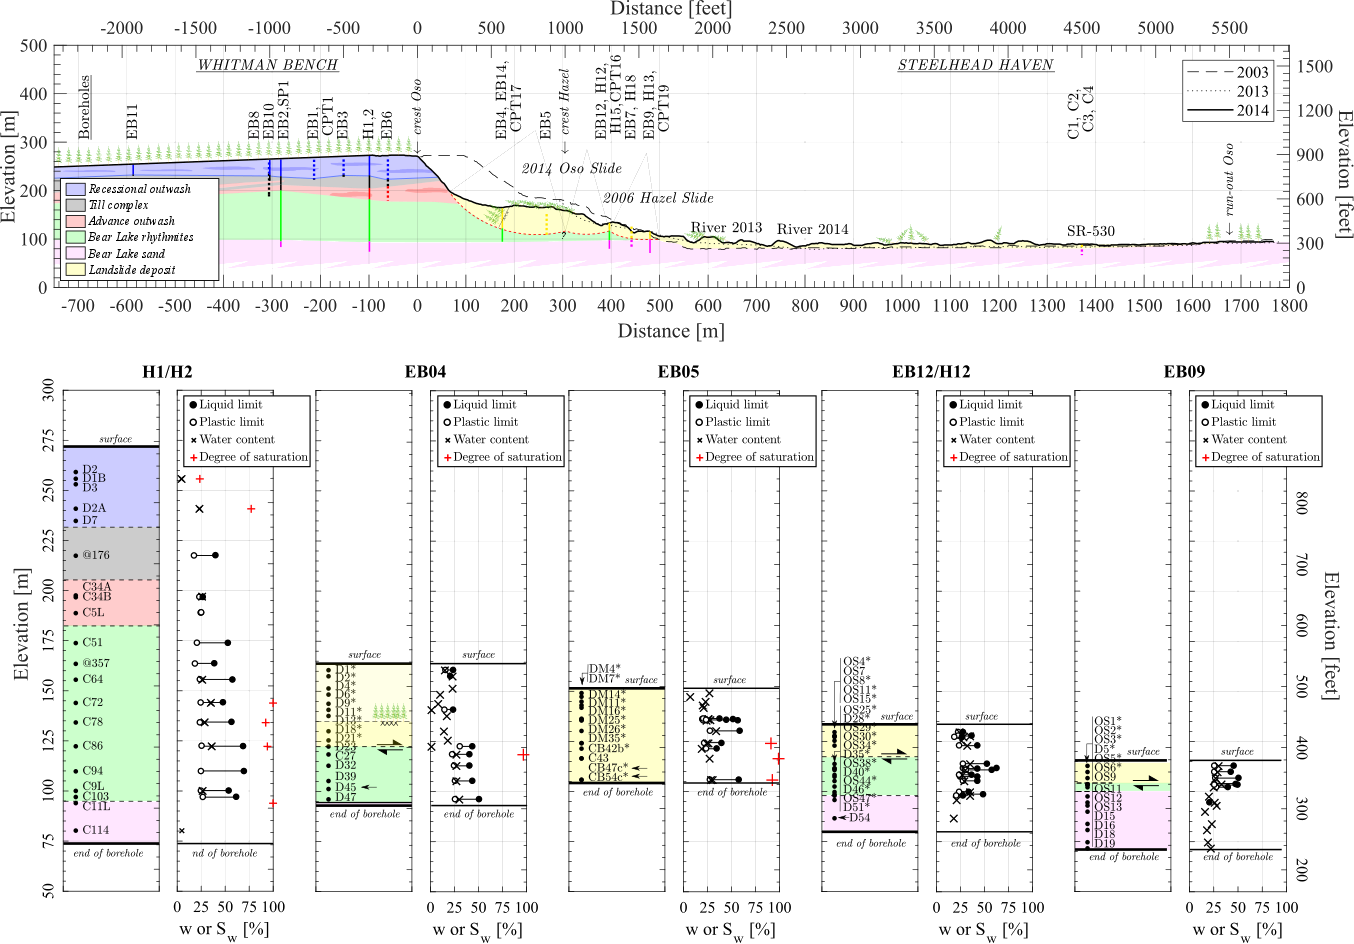
\includegraphics[width=0.9\textwidth]{figs/oso/soil.png}
	\end{figure}
\end{frame}

%------------------------------------------------
\begin{frame}
	\frametitle{Oso landslide: Geology. Identify the failure surface}
	\begin{figure}
		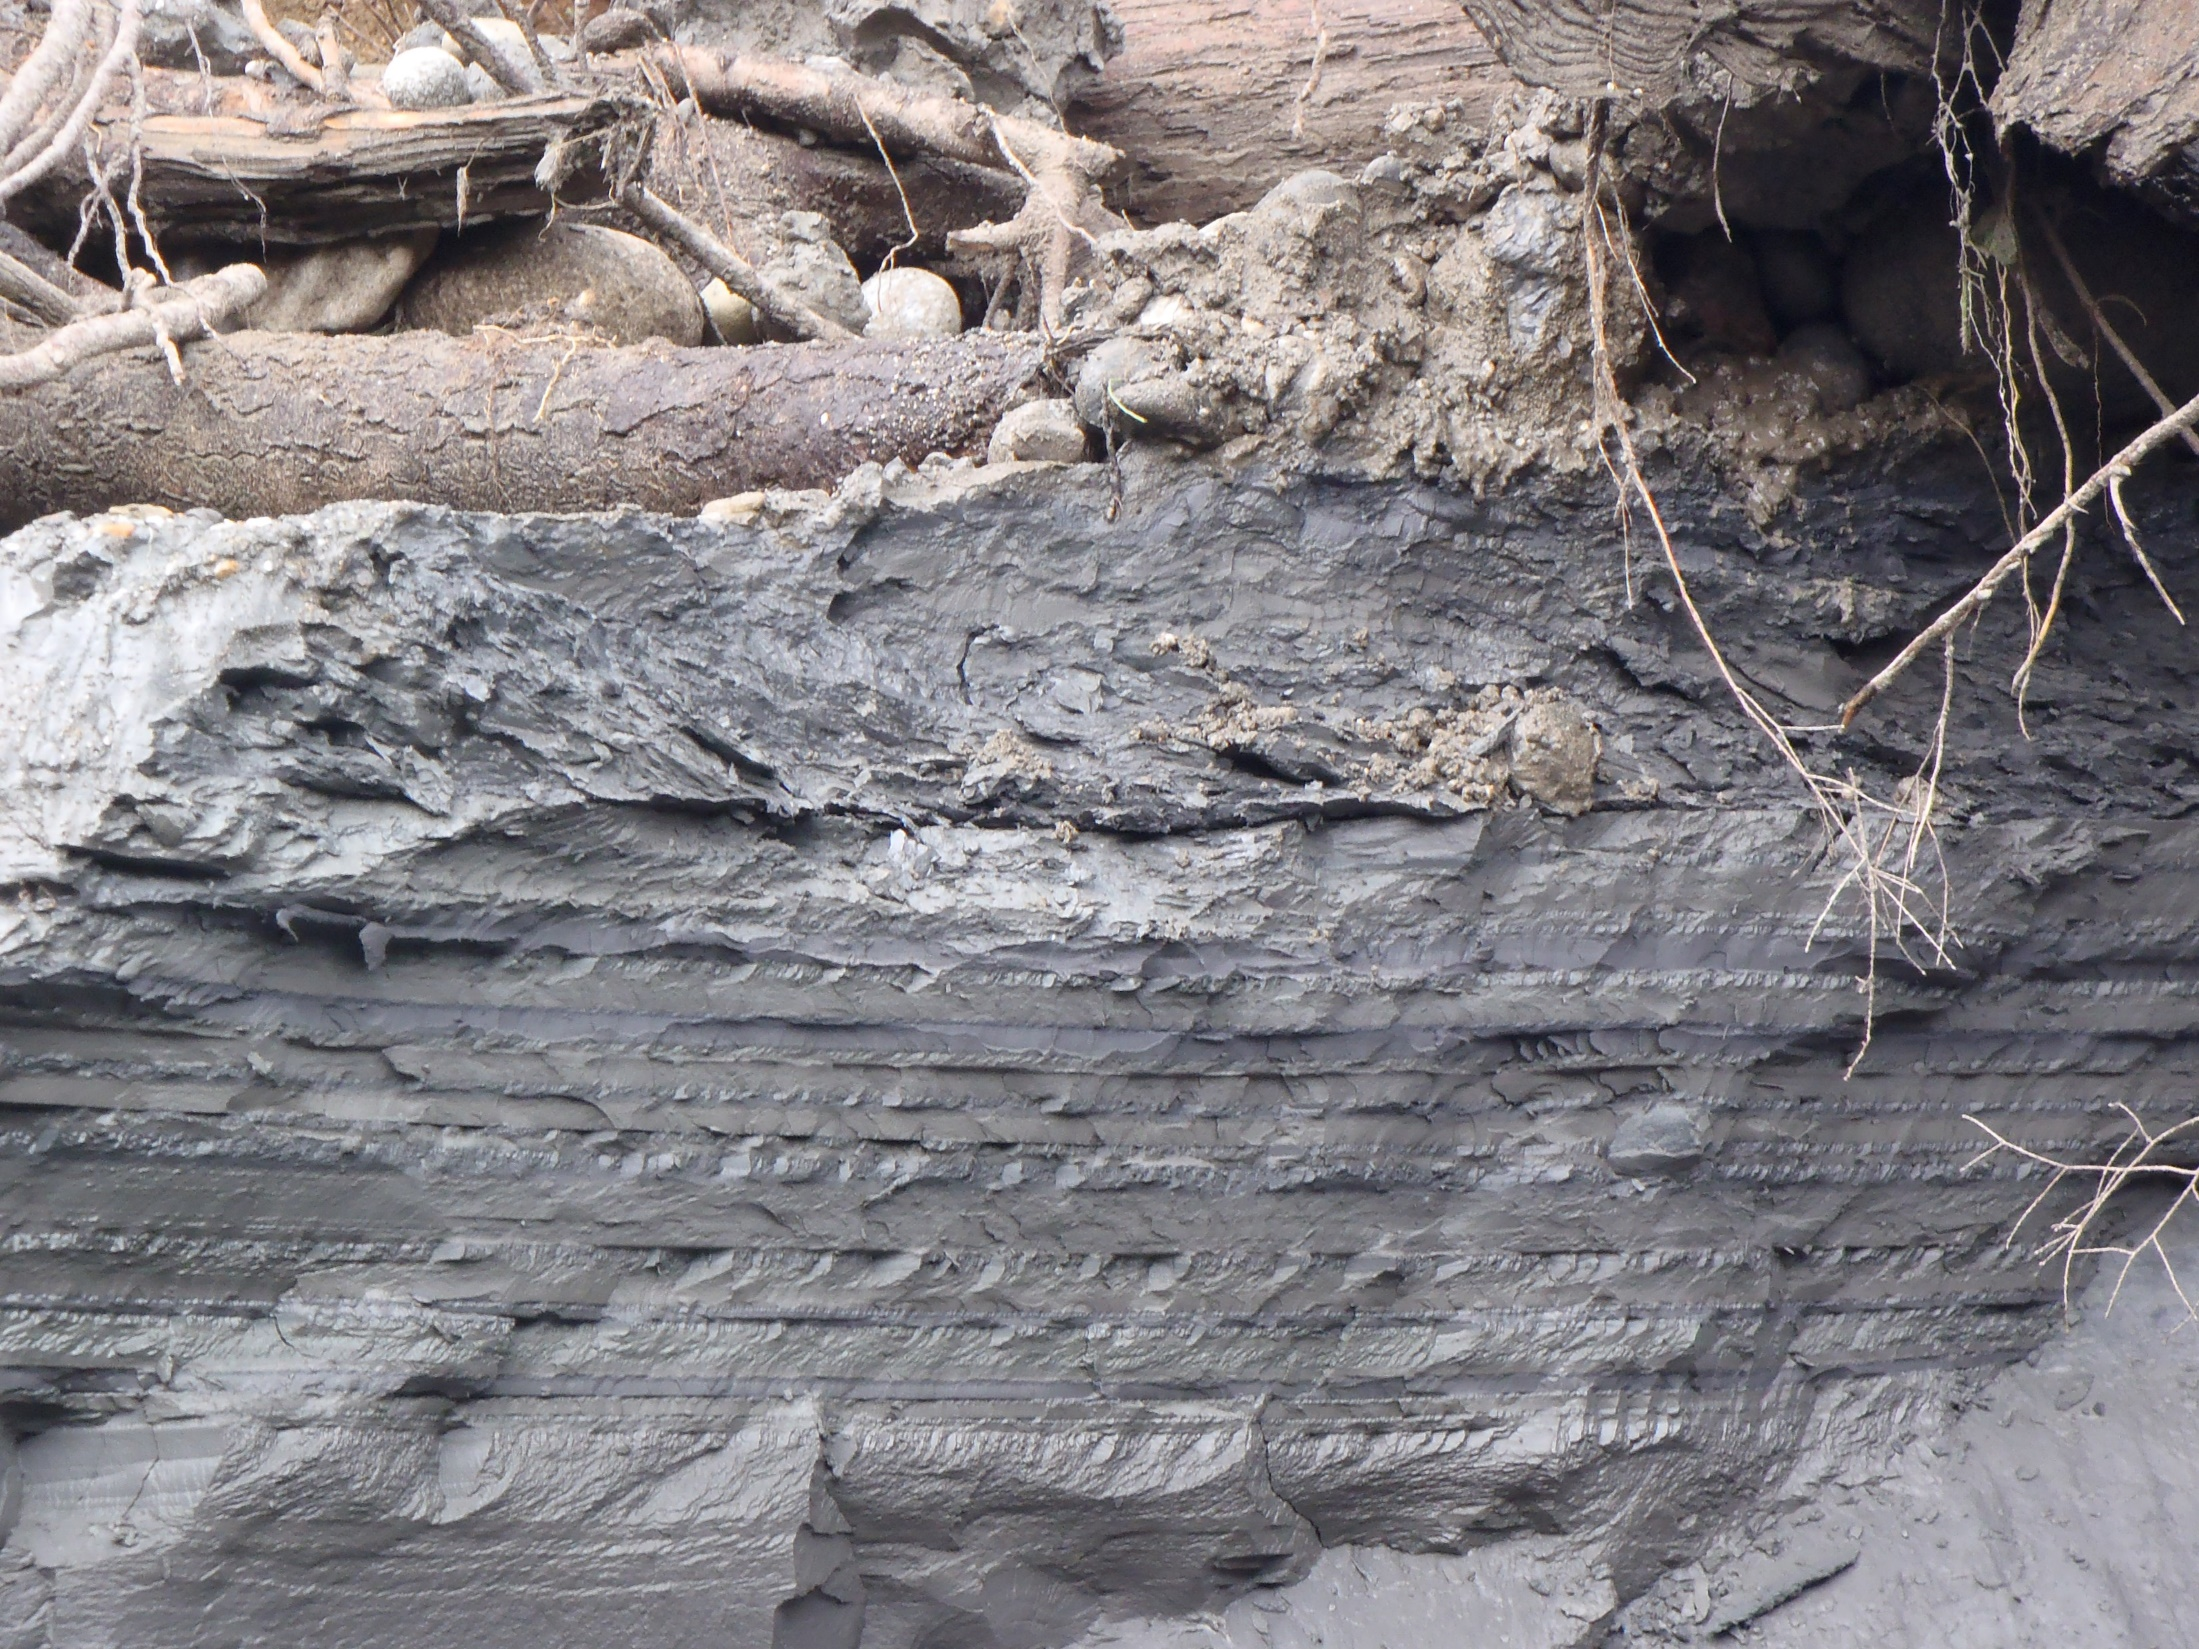
\includegraphics[width=0.75\textwidth]{figs/oso/slip-surface.jpeg}
		\caption*{Lower portion of Bear Lake Rhythmites with failure surface. Courtesy of Dr Gunnar Schlieder}
	\end{figure}
\end{frame}

%------------------------------------------------
\begin{frame}
	\frametitle{Oso landslide: Geology}
	\begin{figure}
		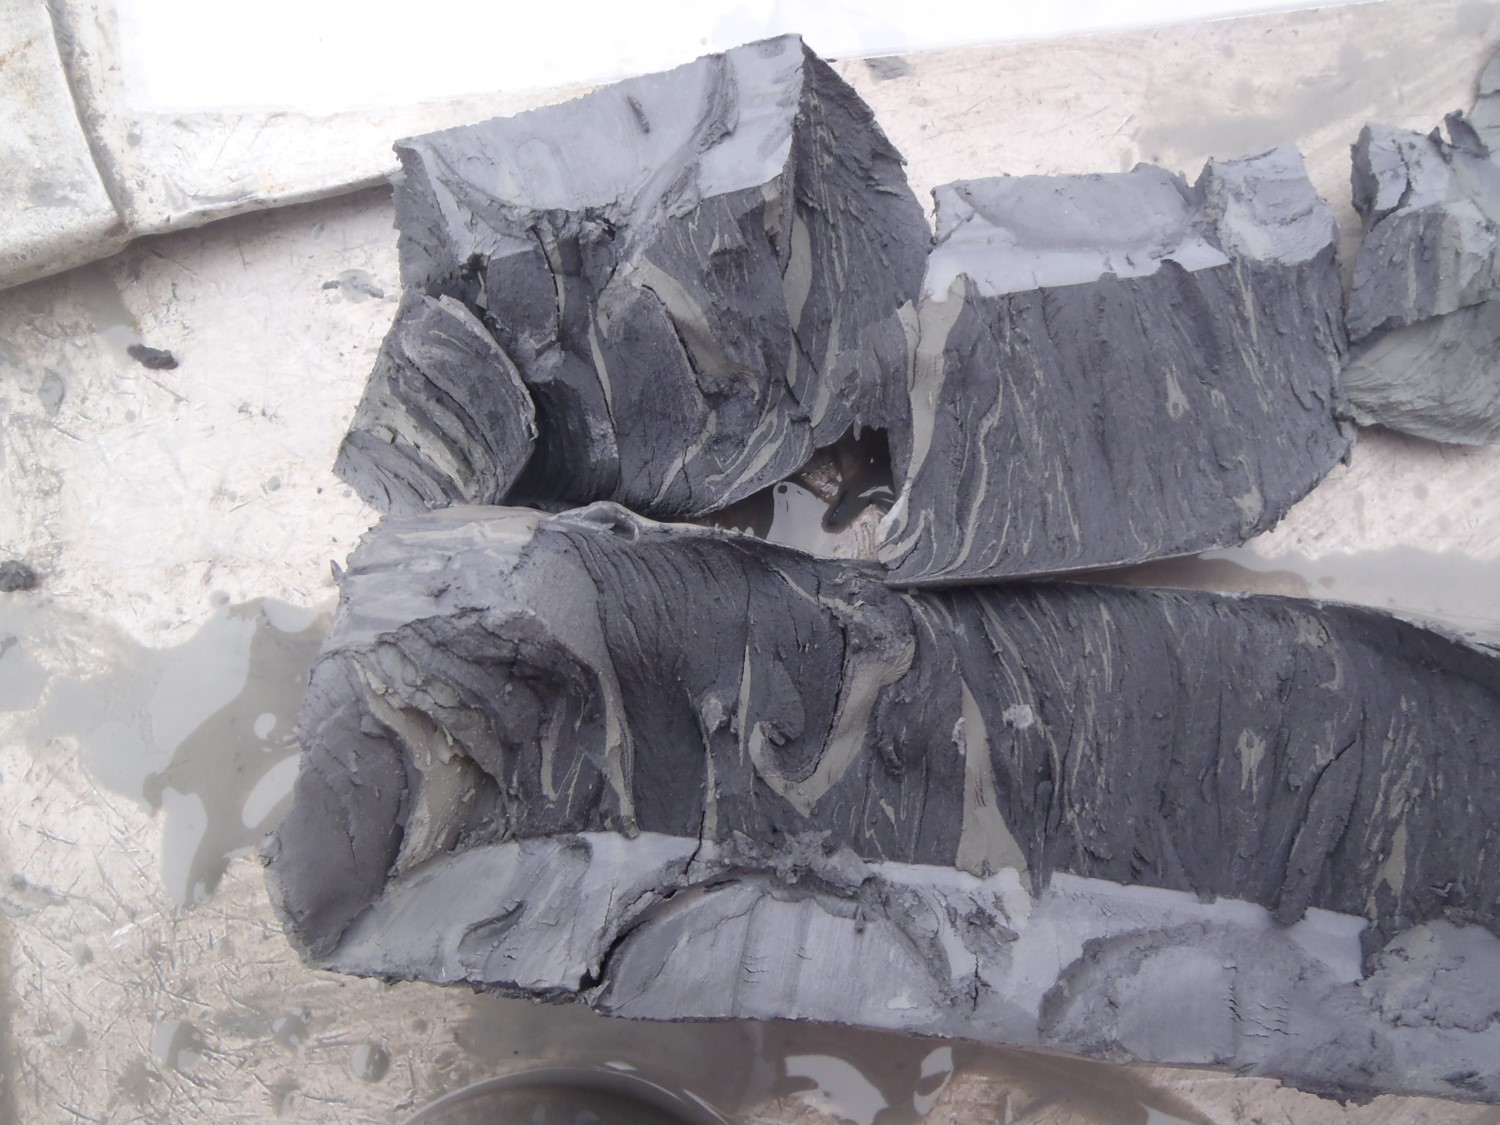
\includegraphics[width=0.75\textwidth]{figs/oso/flame-structures.jpg}
		\caption*{Deformation till with flame structures in fine-grained glacio-lacustrine deposit EB7 (depth 65 ft). Courtesy of Dr Gunnar Schlieder}
	\end{figure}
\end{frame}



%------------------------------------------------
\begin{frame}
	\frametitle{Oso landslide: Direct shear test (intact specimens)}
	\noindent
	\fboxsep=0pt
	\noindent
	\begin{minipage}[t]{0.65\linewidth}
		\begin{itemize}
			\item \textbf{Peak strength (effective stress)}
			\begin{itemize}
				\item Friction angle $\phi^\prime_{max} = 24^o (> \phi^\prime_{cs} = 22^o)$
				\item Cohesion $c^\prime_{max} = 100 kPa (> c^\prime_{cs} = 0)$
			\end{itemize}
				\item \textbf{But some specimens}
			\begin{itemize}
				\item Friction angle $\phi^\prime_{max} = 12^o (< \phi^\prime_{cs} = 22^o)$
				\item Cohesion $c^\prime_{max} = 0 kPa ( = c^\prime_{cs})$
			\end{itemize}
			\item Natural soil with structure
			\begin{itemize}
				\item Is it an intrinsic material property?
				\item Or a soil structure property?
			\end{itemize}
		\end{itemize}
		
	\end{minipage}%
	\hfill
	\begin{minipage}[t]{0.35\linewidth}
	\begin{figure}
		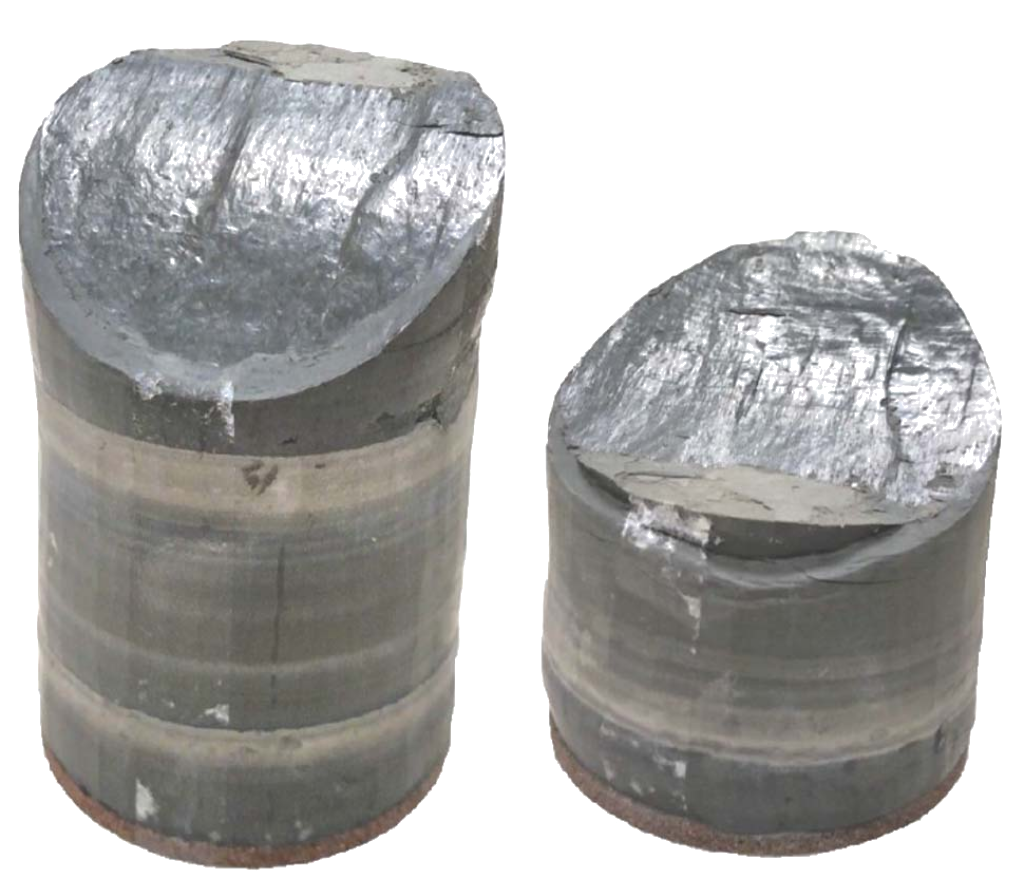
\includegraphics[width=\textwidth]{figs/oso/direct-shear-test.png}
	\end{figure}
	\end{minipage}	
\end{frame}

%------------------------------------------------
\begin{frame}
	\frametitle{Oso landslide: Analysis}
	\begin{figure}
		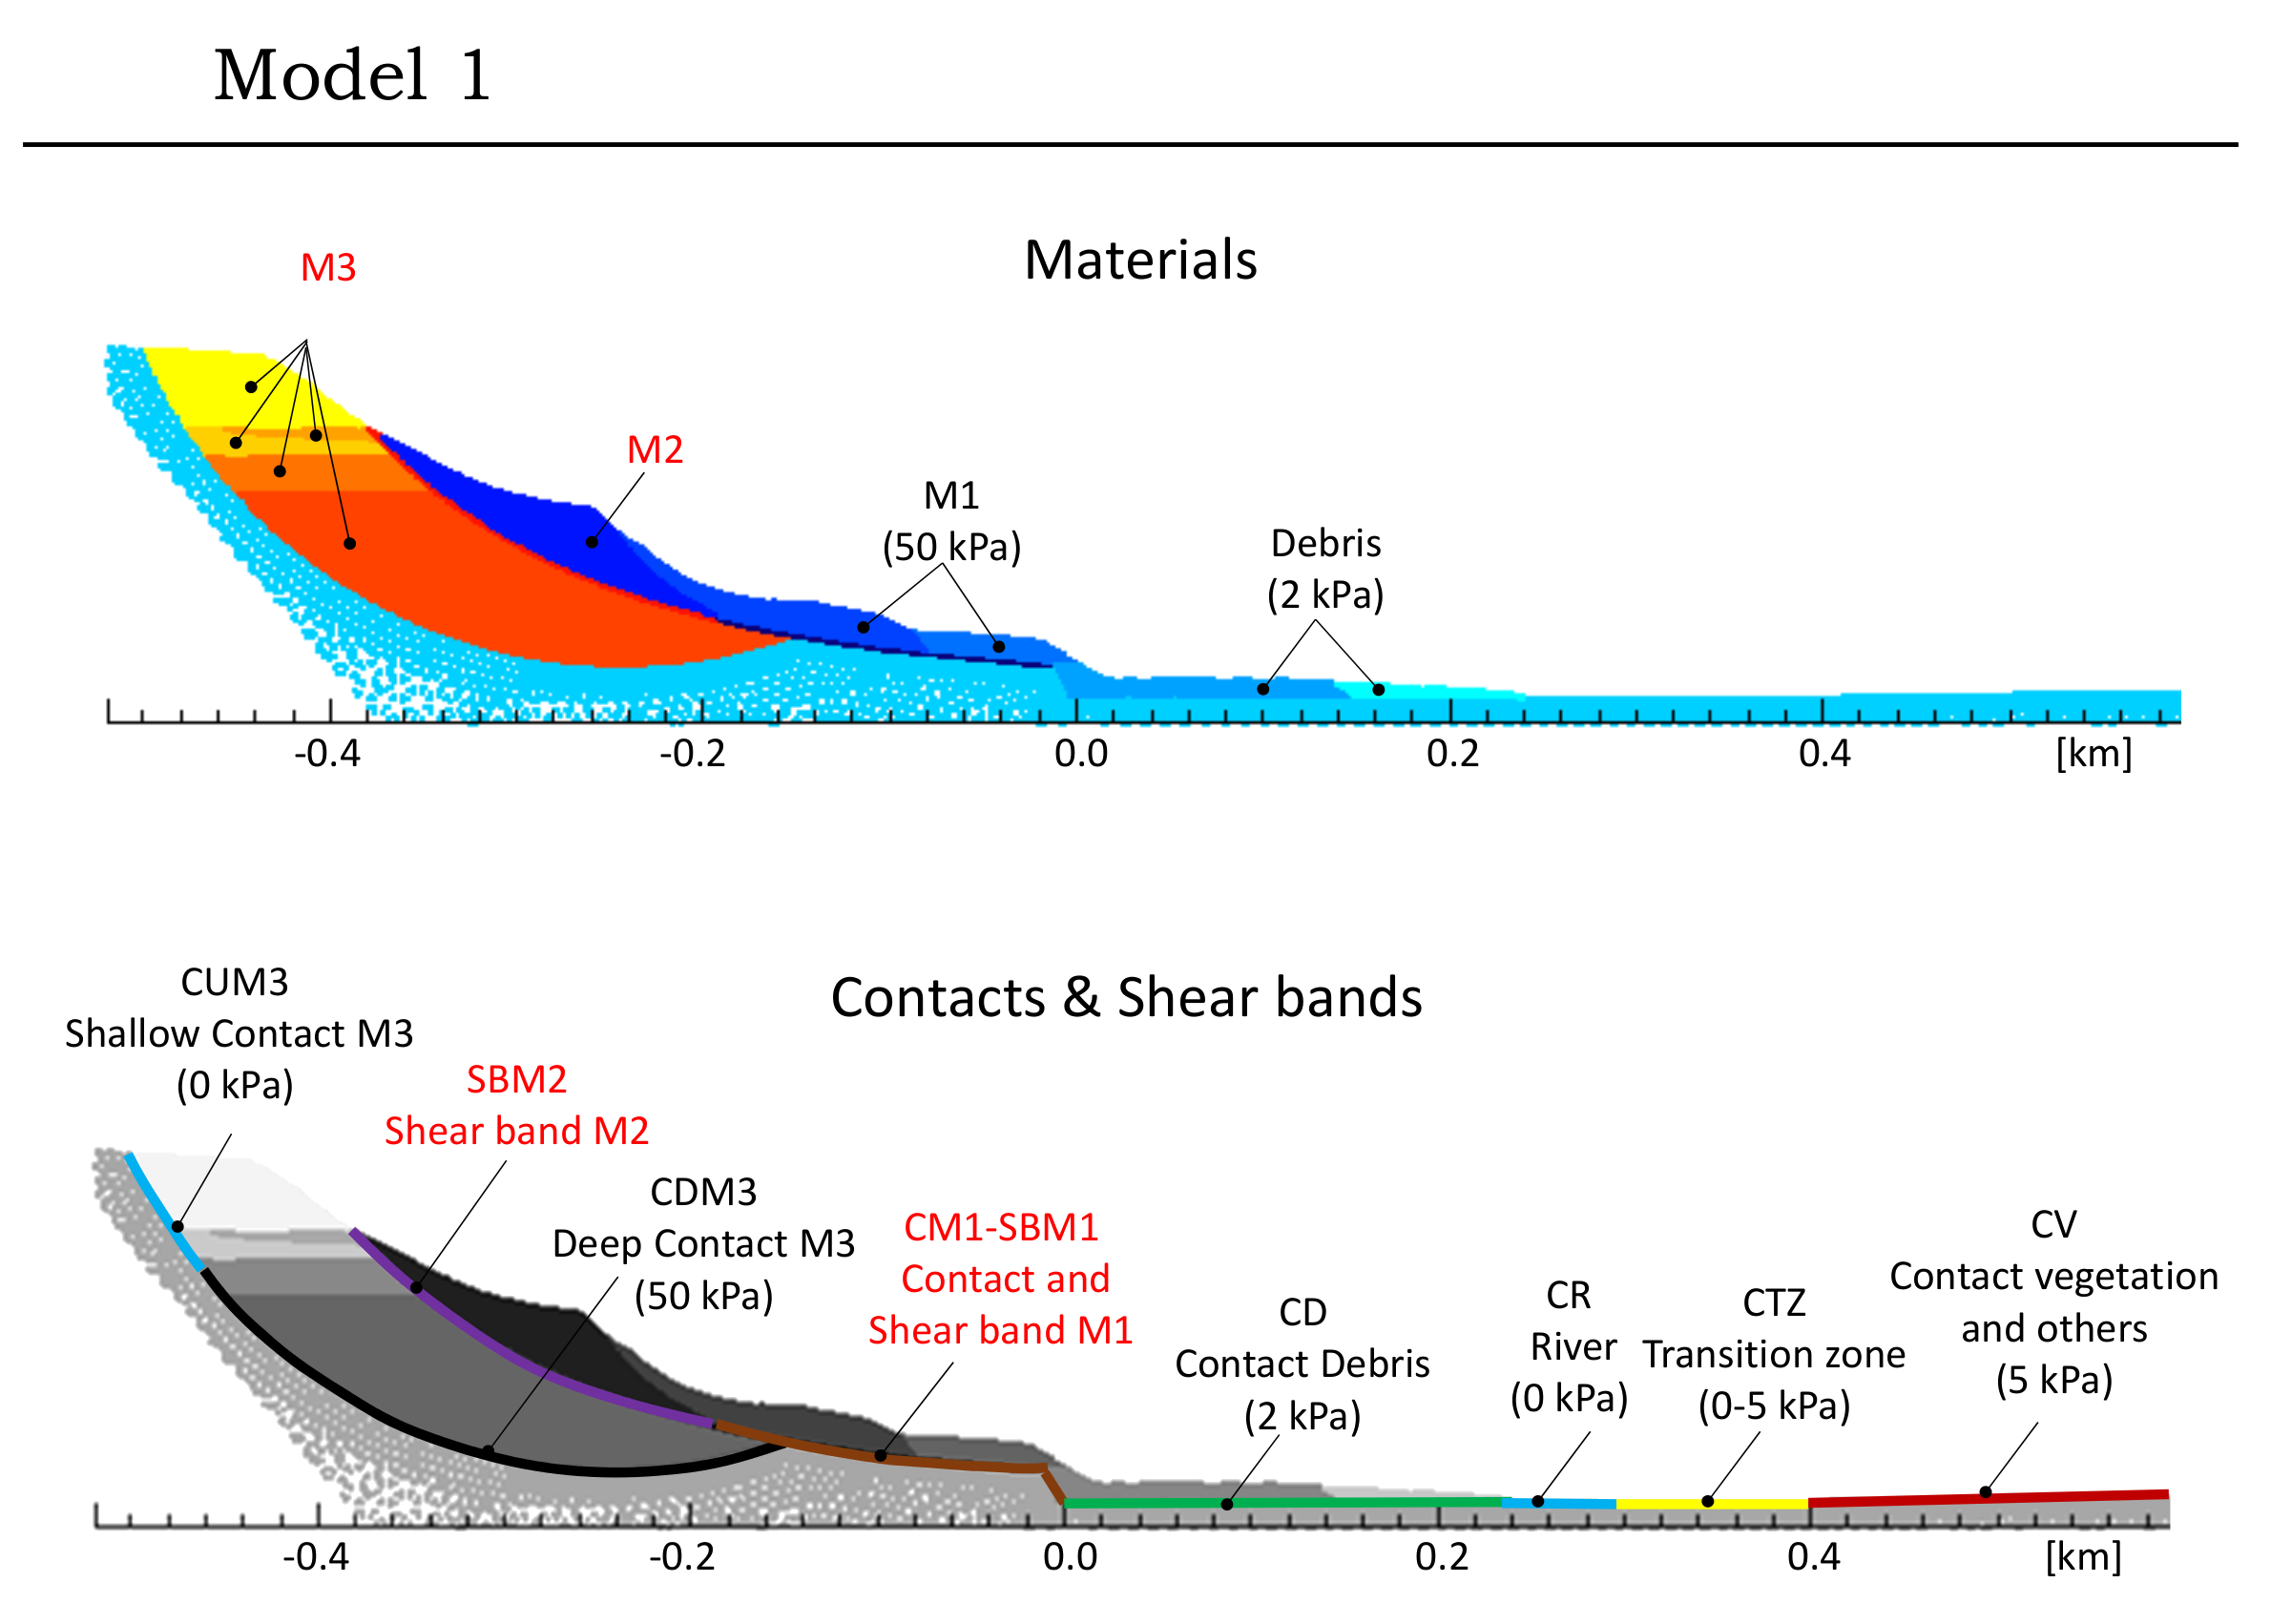
\includegraphics[width=0.85\textwidth]{figs/oso/mpm-setup.png}
		\caption*{Alba et al., 2018}
	\end{figure}
\end{frame}

%------------------------------------------------
\begin{frame}
	\frametitle{Oso landslide: Analysis}
	\begin{figure}
		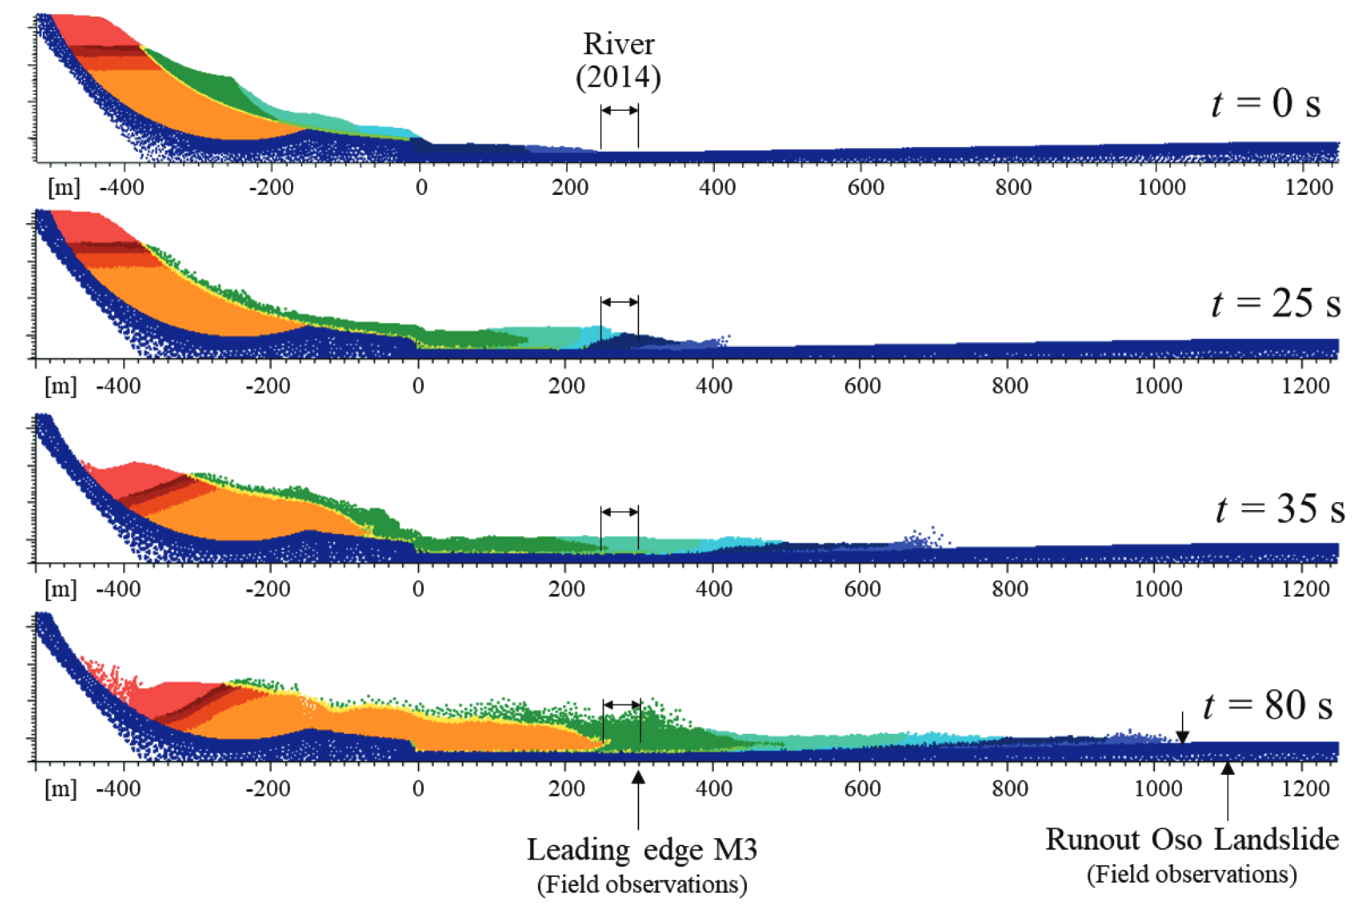
\includegraphics[width=0.85\textwidth]{figs/oso/oso-simulation.png}
		\caption*{Alba et al., 2018}
	\end{figure}
\end{frame}

\section{Geotechnical analysis}
%------------------------------------------------
\begin{frame}
\frametitle{Advanced analysis in geotechnical engineering}
Geotechnical design:
\mode<beamer>{
	\begin{itemize}
		\item Assess applied forces
		\item evaluate ``performance" (stability \& movements) under working and ultimate loads
	\end{itemize}
}
\mode<handout>{
	\vspace{3cm}
}
Analysis:
\mode<beamer>{
	\begin{itemize}
		\item Mathematical framework to perform calculations for these quantities
		\item Requires idealization of: geometry, soil properties, and loading conditions
		\item Analysis is a tool in design, but design involves more: acceptable movements, constraints, site characterization, etc.
	\end{itemize}
}
\mode<handout>{
	\vspace{3cm}
}
\end{frame}
\note{As part of the design process, it is necessary for an engineer to perform 
	calculations to provide estimates of the above quantities. Analysis provides 
	the mathematical framework for such calculations. A good analysis, which 
	simulates real behaviour, allows the engineer to understand problems better. While an
	important part of the design process, analysis only provides the engineer with a
	tool to quantify effects once material properties and loading conditions have been
	set. The design process involves considerably more than analysis.}

%------------------------------------------------
\begin{frame}
	\frametitle{Classical geotechnical analysis: Slope stability}
	\mode<beamer>{
		\noindent
		\fboxsep=0pt
		\noindent
		\begin{minipage}[t]{0.6\linewidth}	
			\textbf{Assumptions}
			\begin{itemize}
				\item  \textit{Mode:} Assume failure surface
				\item \textit{Deformation:} Rigid soil block
				\item \textit{Slip surface:} Define a failure criteria
				\item \textit{Compute:} $F_s$ Stability
			\end{itemize}
			This is the classical \textbf{limit equilibrium method}.
		\end{minipage}%
		\hfill
		\begin{minipage}[t]{0.4\linewidth}
			\begin{figure}
				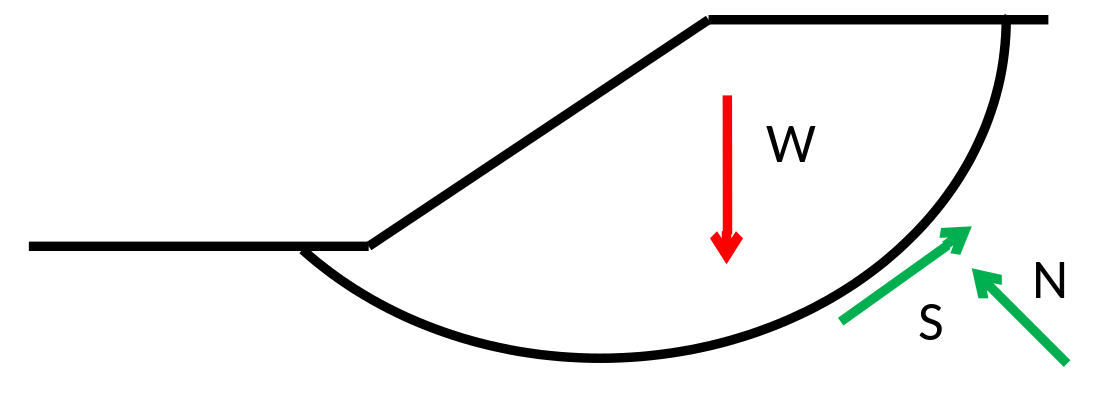
\includegraphics[width=\textwidth]{figs/limit-equilibrium.png}
			\end{figure}
		\end{minipage}	
	}
	\mode<handout>{
		\vspace{5cm}
	}
\end{frame}
\note {Limit equilibrium
	In this method of analysis an 'arbitrary' failure surface is adopted (assumed) and
	equilibrium conditions are considered for the failing soil mass, assuming that the
	failure criterion holds everywhere along the failure surface. The failure surface
	may be planar, curved or some combination of these. Only the global equilibrium
	of the `blocks' of soil between the failure surfaces and the boundaries of the
	problem are considered. The internal stress distribution within the blocks of soil is
	not considered. Coulomb's wedge analysis and the method of slices are examples
	of limit equilibrium calculations. \\
	
	Only a global equilibrium, rather than the local equilibirium of every point in the soil, is satisified.
}

%------------------------------------------------
\begin{frame}
	\frametitle{Shear failure plane}
	\begin{figure}[ht]
		\centering
		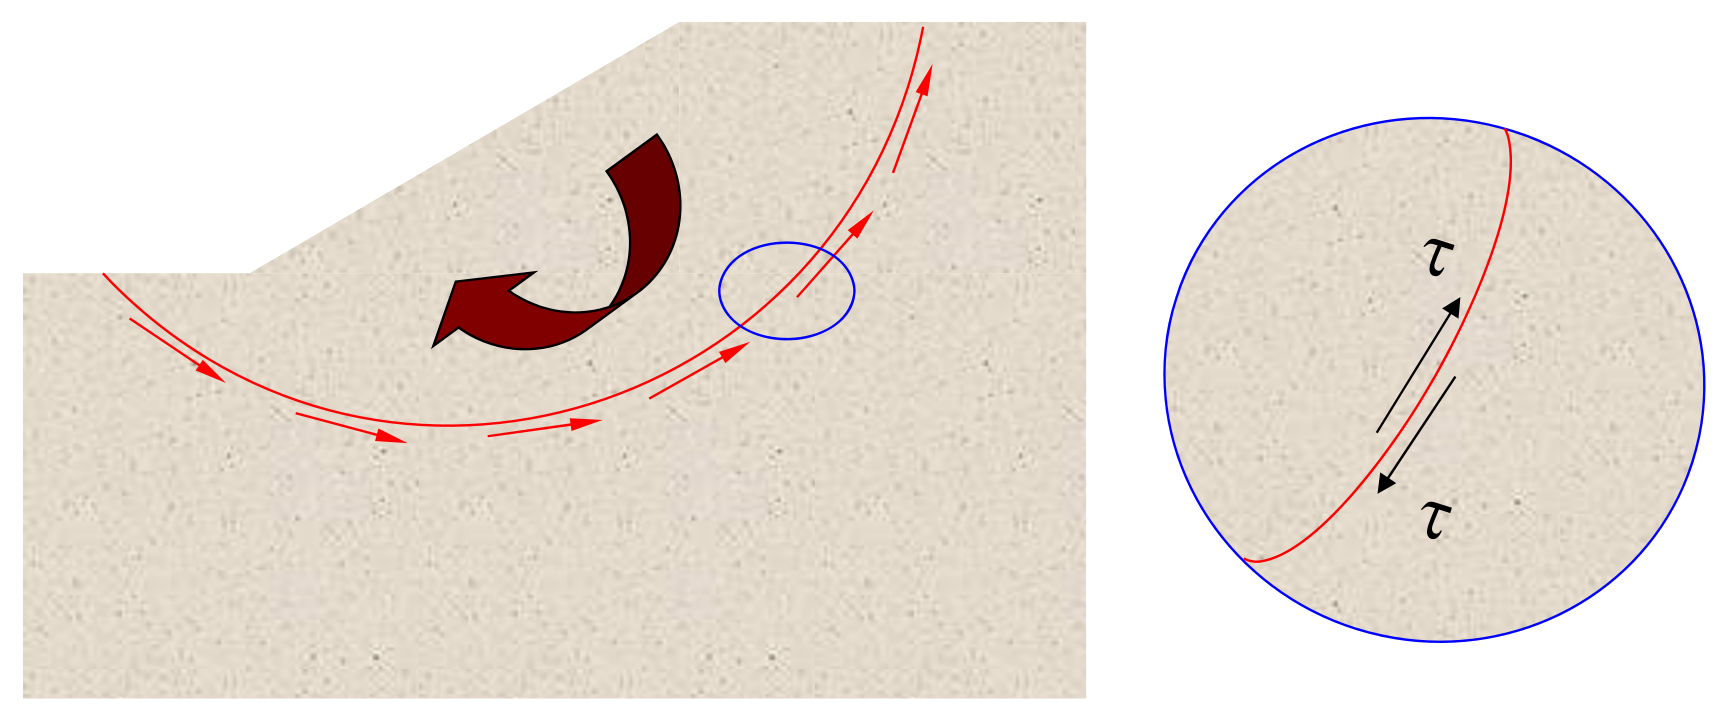
\includegraphics[width=0.9\textwidth]{figs/shear-failure-plane.png}
		\caption*{At failure, shear stress along the failure surface ($\tau$) reaches the shear strength ($\tau_f$).}
	\end{figure}
	Factor of Safety = \mode<beamer>{Resistance (from soil shear strength)/Driving force (from total
		stress equilibrium (i.e. weight of the soil))}
\end{frame}

%------------------------------------------------
\begin{frame}
	\frametitle{Dry slope (total stress = effective stress)}
	\mode<beamer>{
		\begin{figure}[ht]
			\centering
			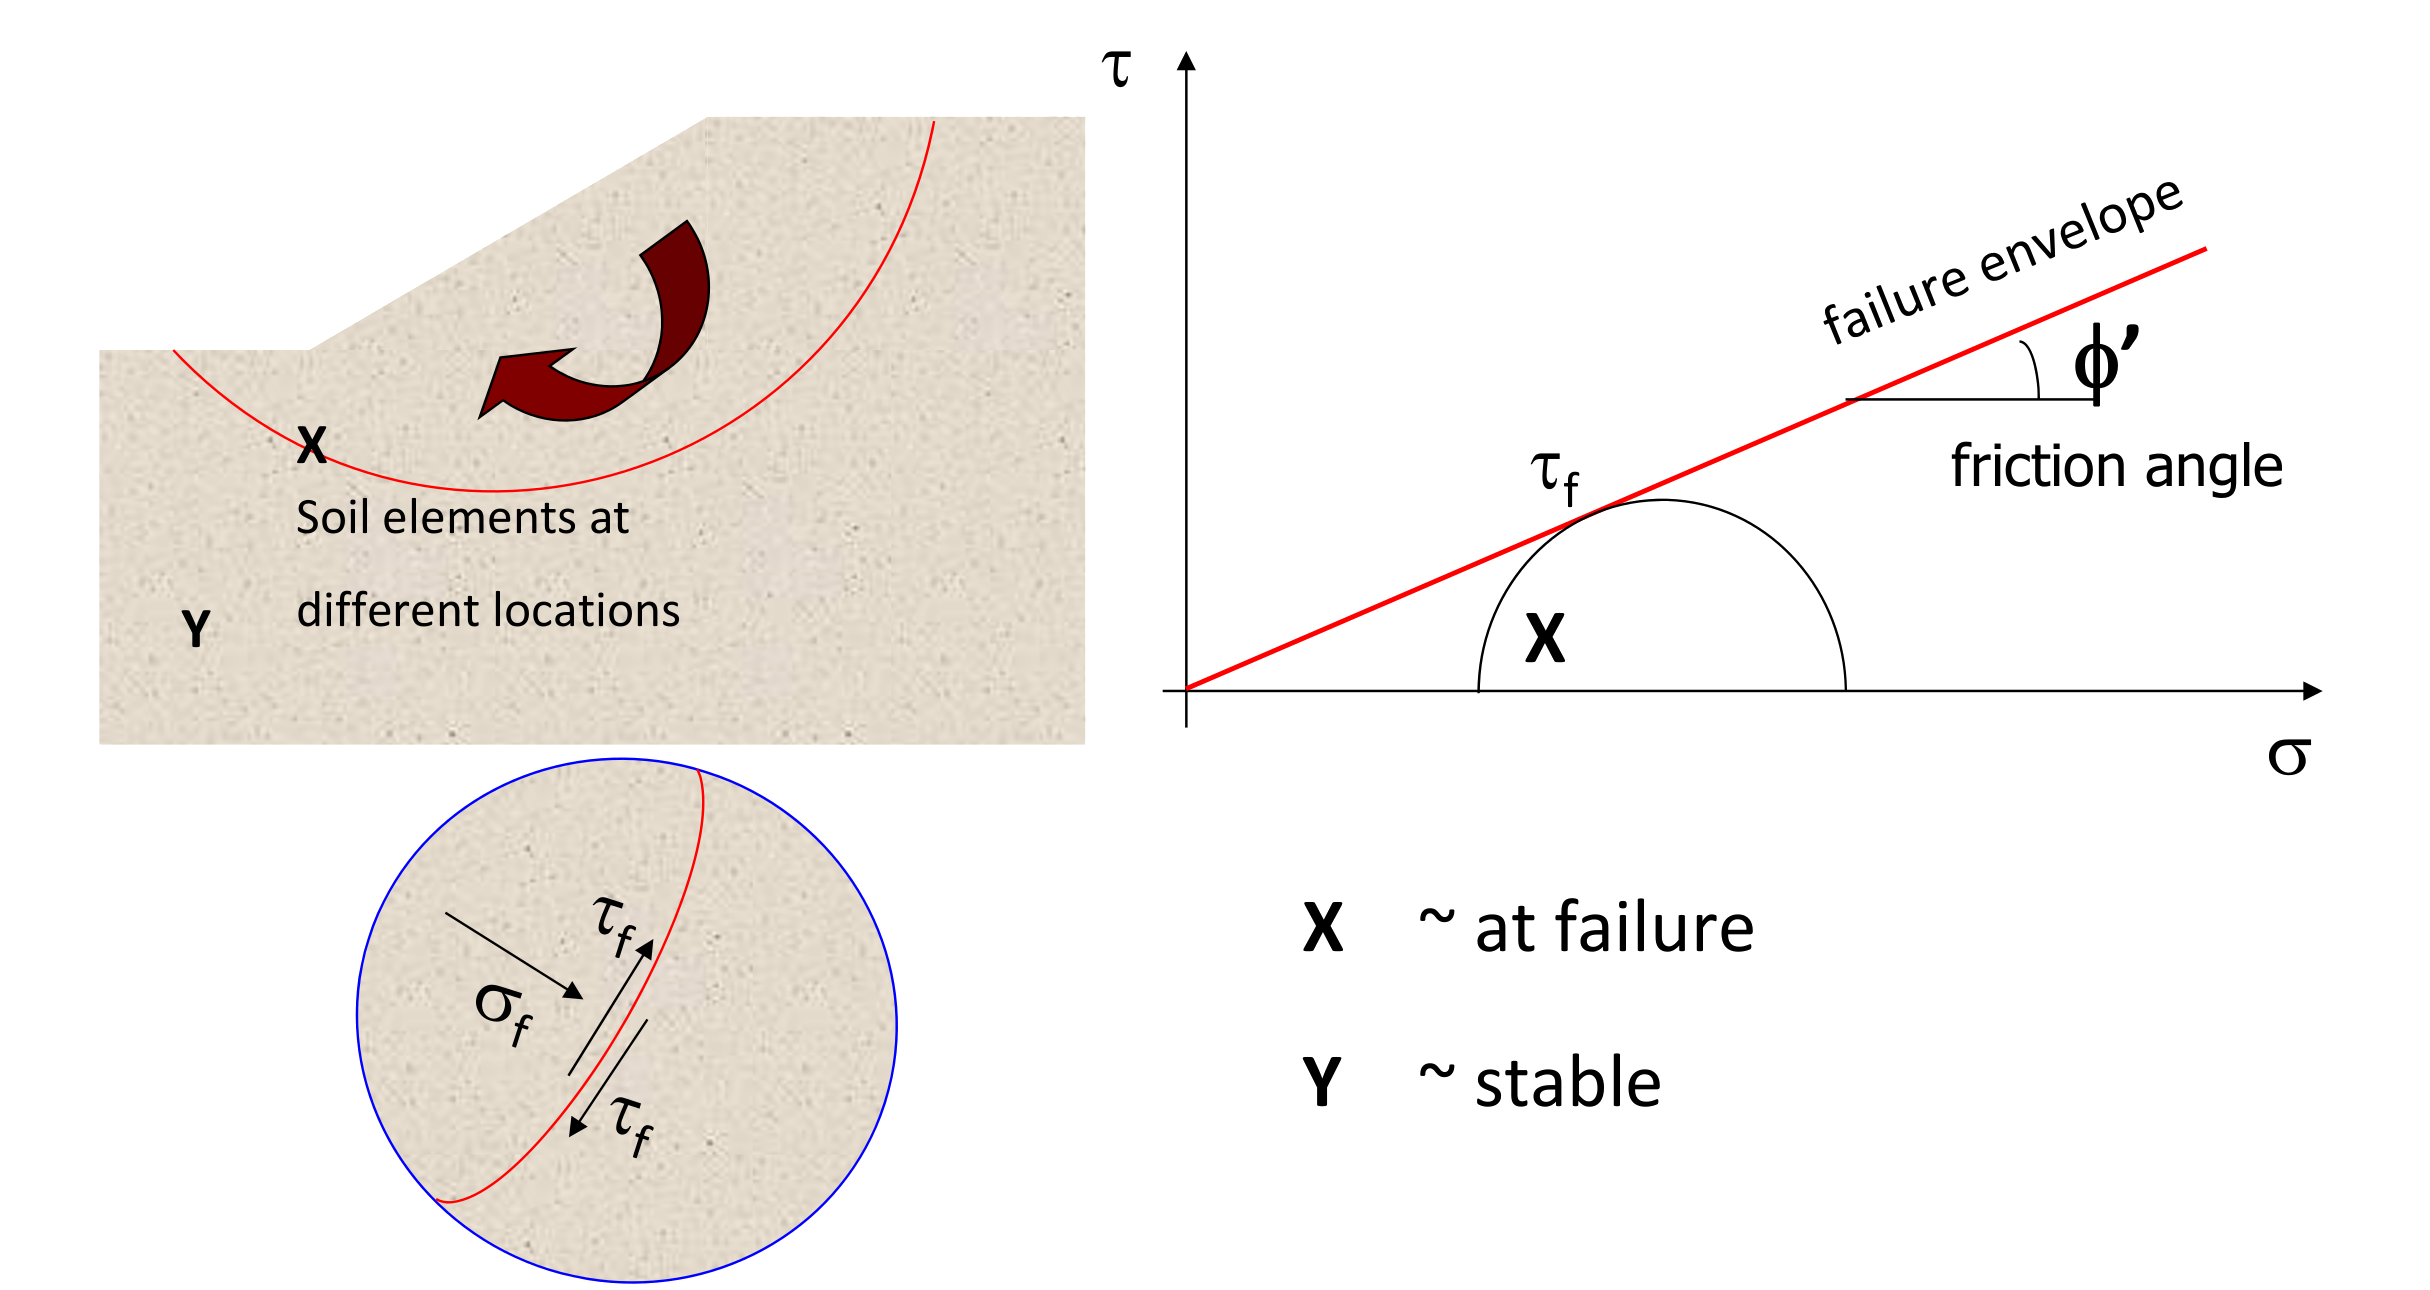
\includegraphics[width=\textwidth]{figs/dry-slope.png}
		\end{figure}
	}
	\mode<handout>{
		\begin{figure}[ht]
			\centering
			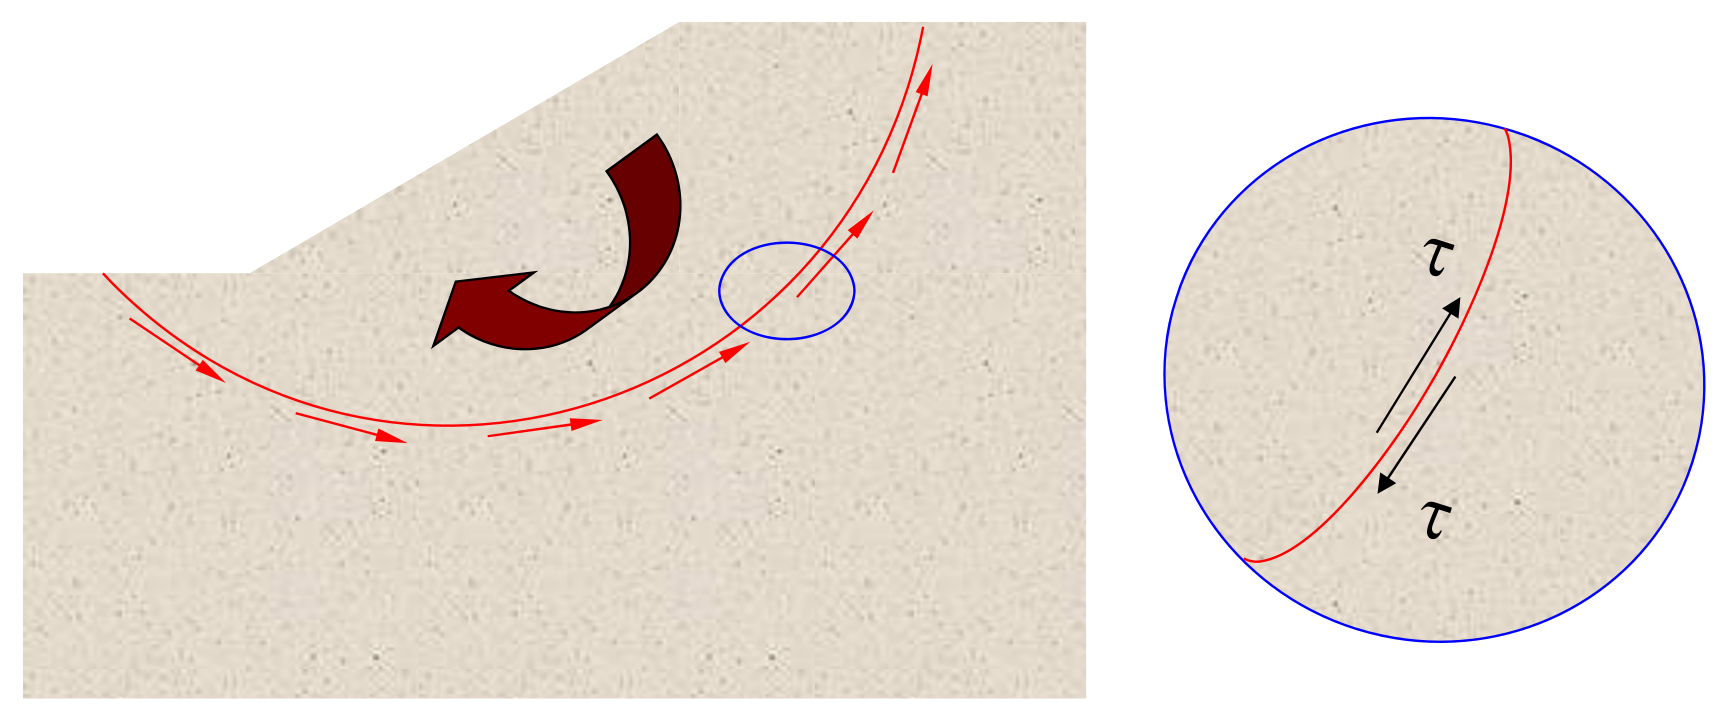
\includegraphics[width=0.9\textwidth]{figs/shear-failure-plane.png}
		\end{figure}
	}
\end{frame}

%------------------------------------------------
\begin{frame}
	\frametitle{Saturated slope (total stress = effective stress + pwp)}
	\textbf{Drained conditions} - need to compute the steady state pore pressure field
	and then evaluate ``effective stress‐based'' shear strength to find the overall
	stability (based on total stress equilibrium).
	\mode<beamer>{
		\begin{figure}[ht]
			\centering
			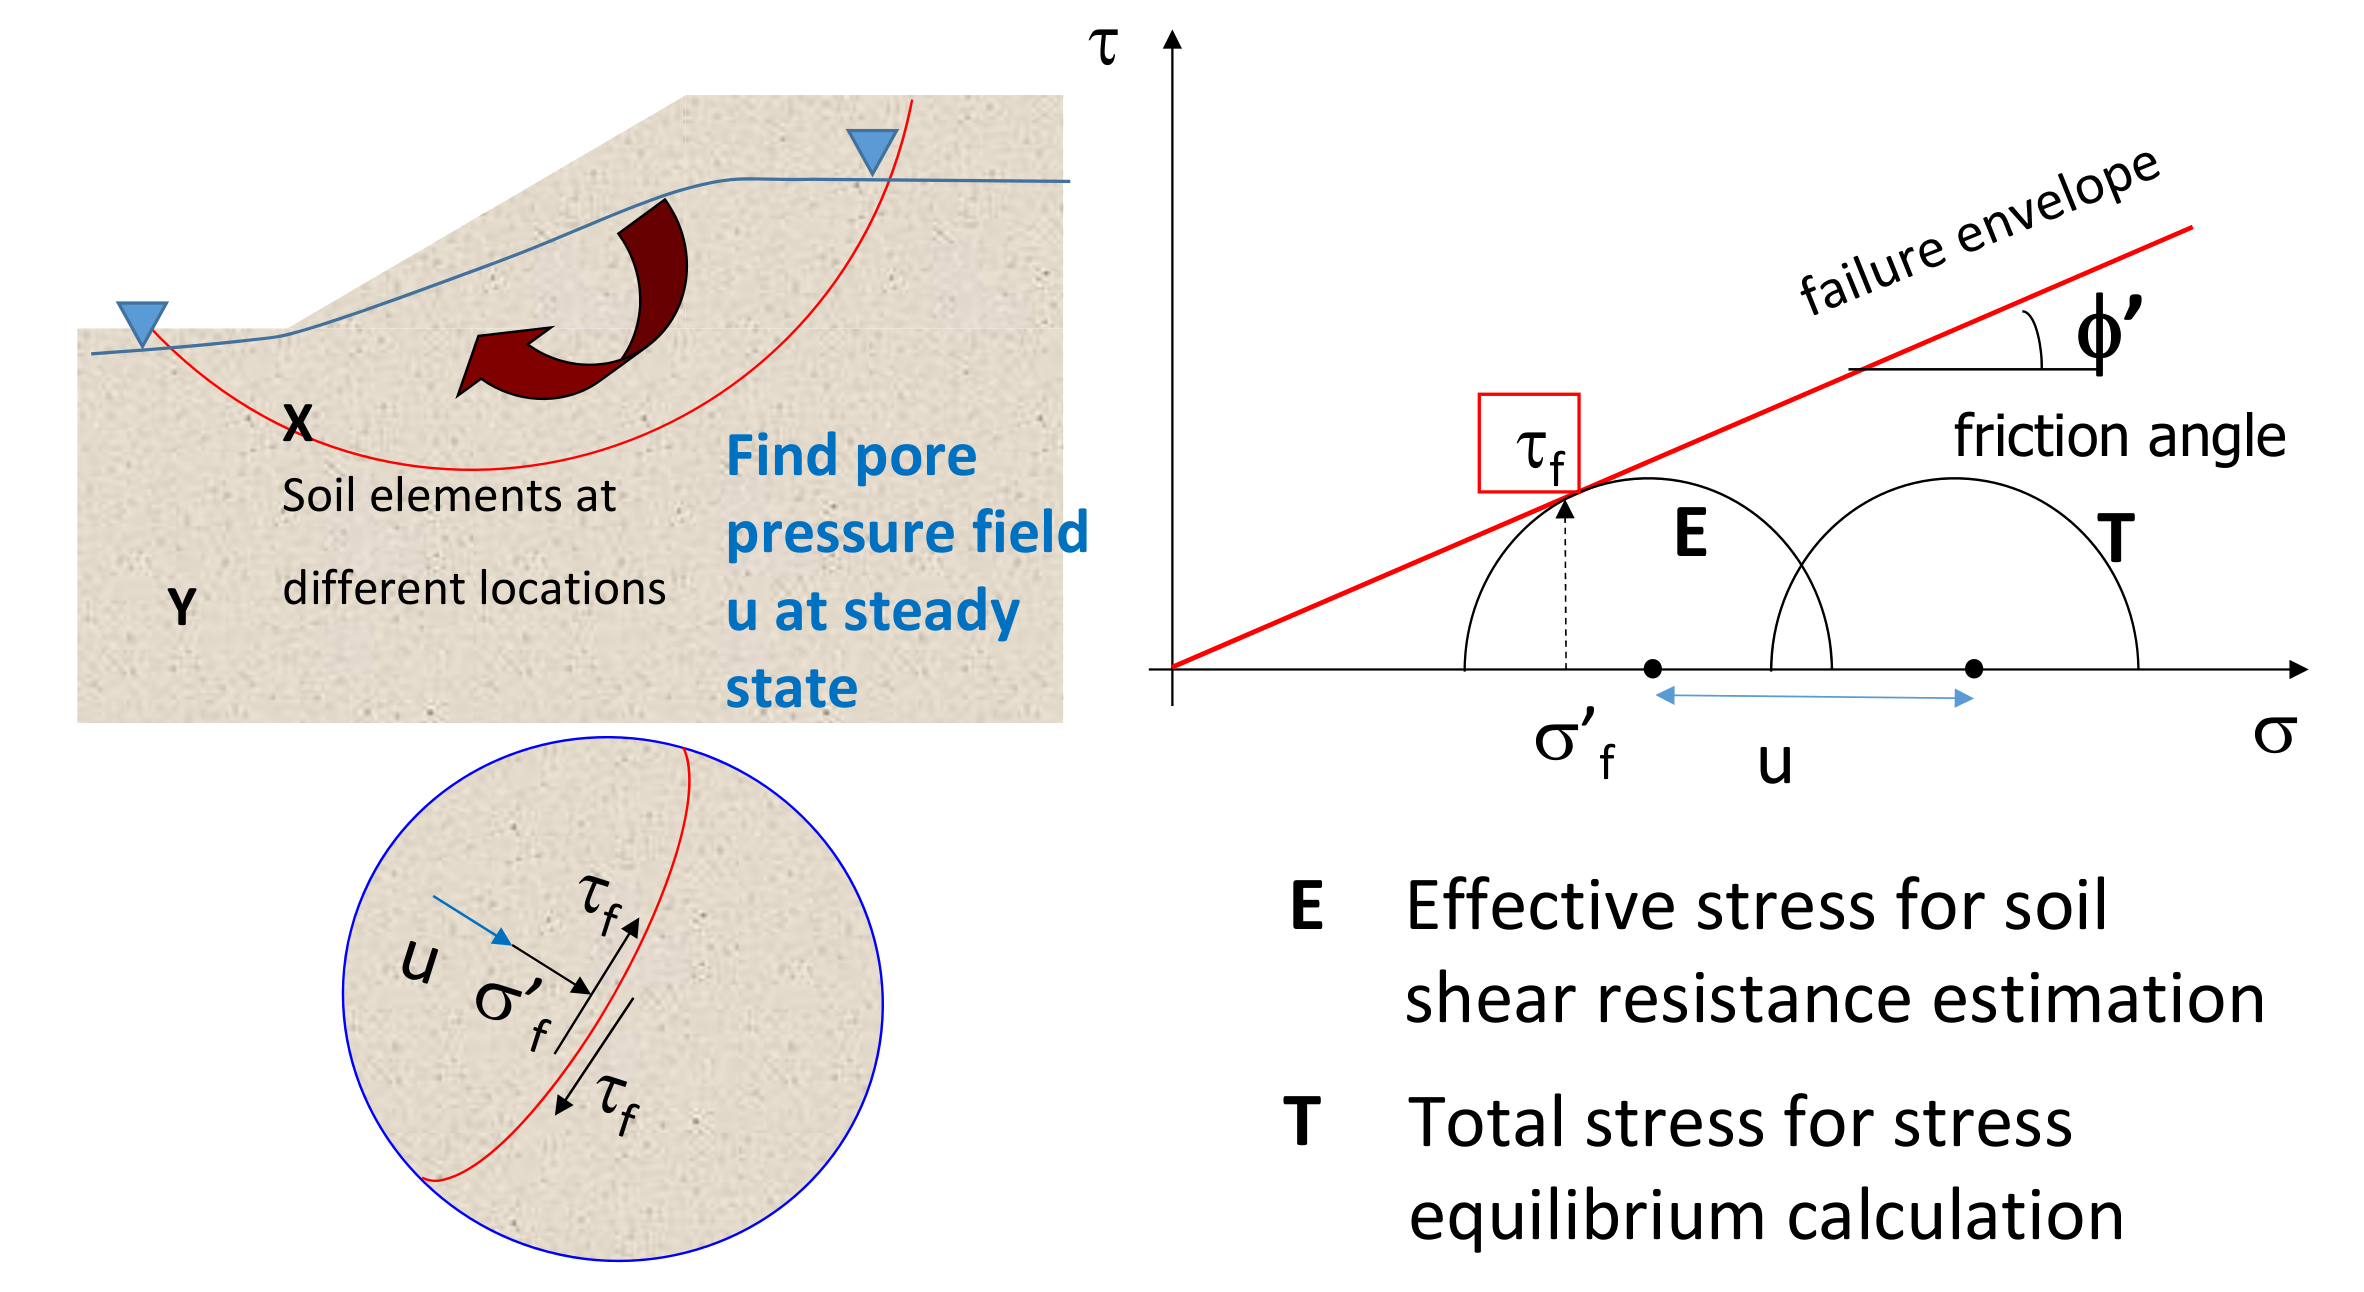
\includegraphics[width=\textwidth]{figs/saturated-slope.png}
		\end{figure}
	}
	\mode<handout>{
		\begin{figure}[ht]
			\centering
			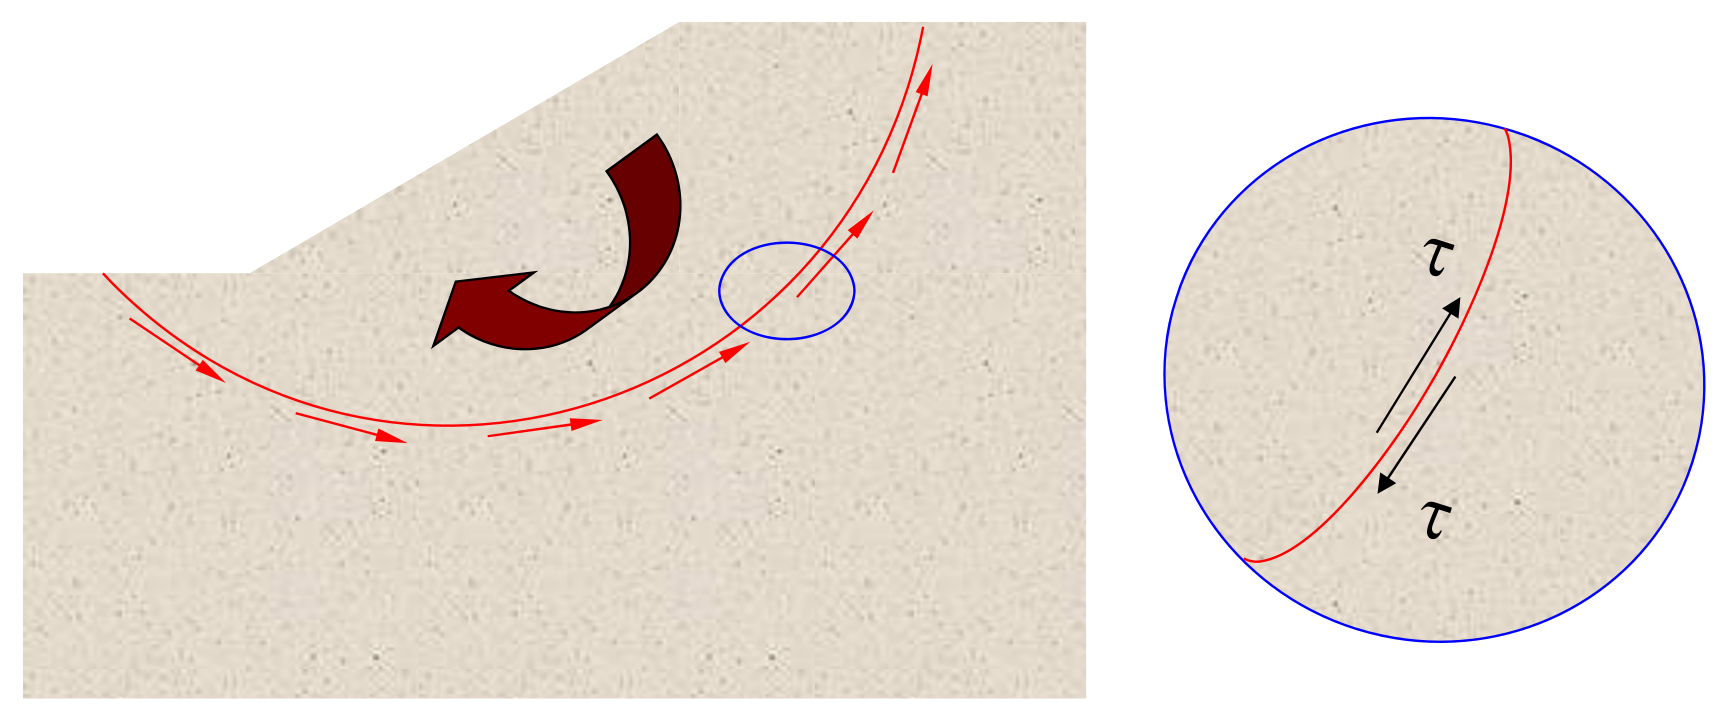
\includegraphics[width=0.9\textwidth]{figs/shear-failure-plane.png}
		\end{figure}
	}
\end{frame}

%------------------------------------------------
\begin{frame}
	\frametitle{Saturated slope (total stress = effective stress + PWP)}
	\textbf{Undrained conditions} ‐ (total stress approach) – Use ``\textit{total‐stress based}''
	shear strength ($s_u$) to find the overall stability (based on total stress
	equilibrium).
	\mode<beamer>{
		\begin{figure}[ht]
			\centering
			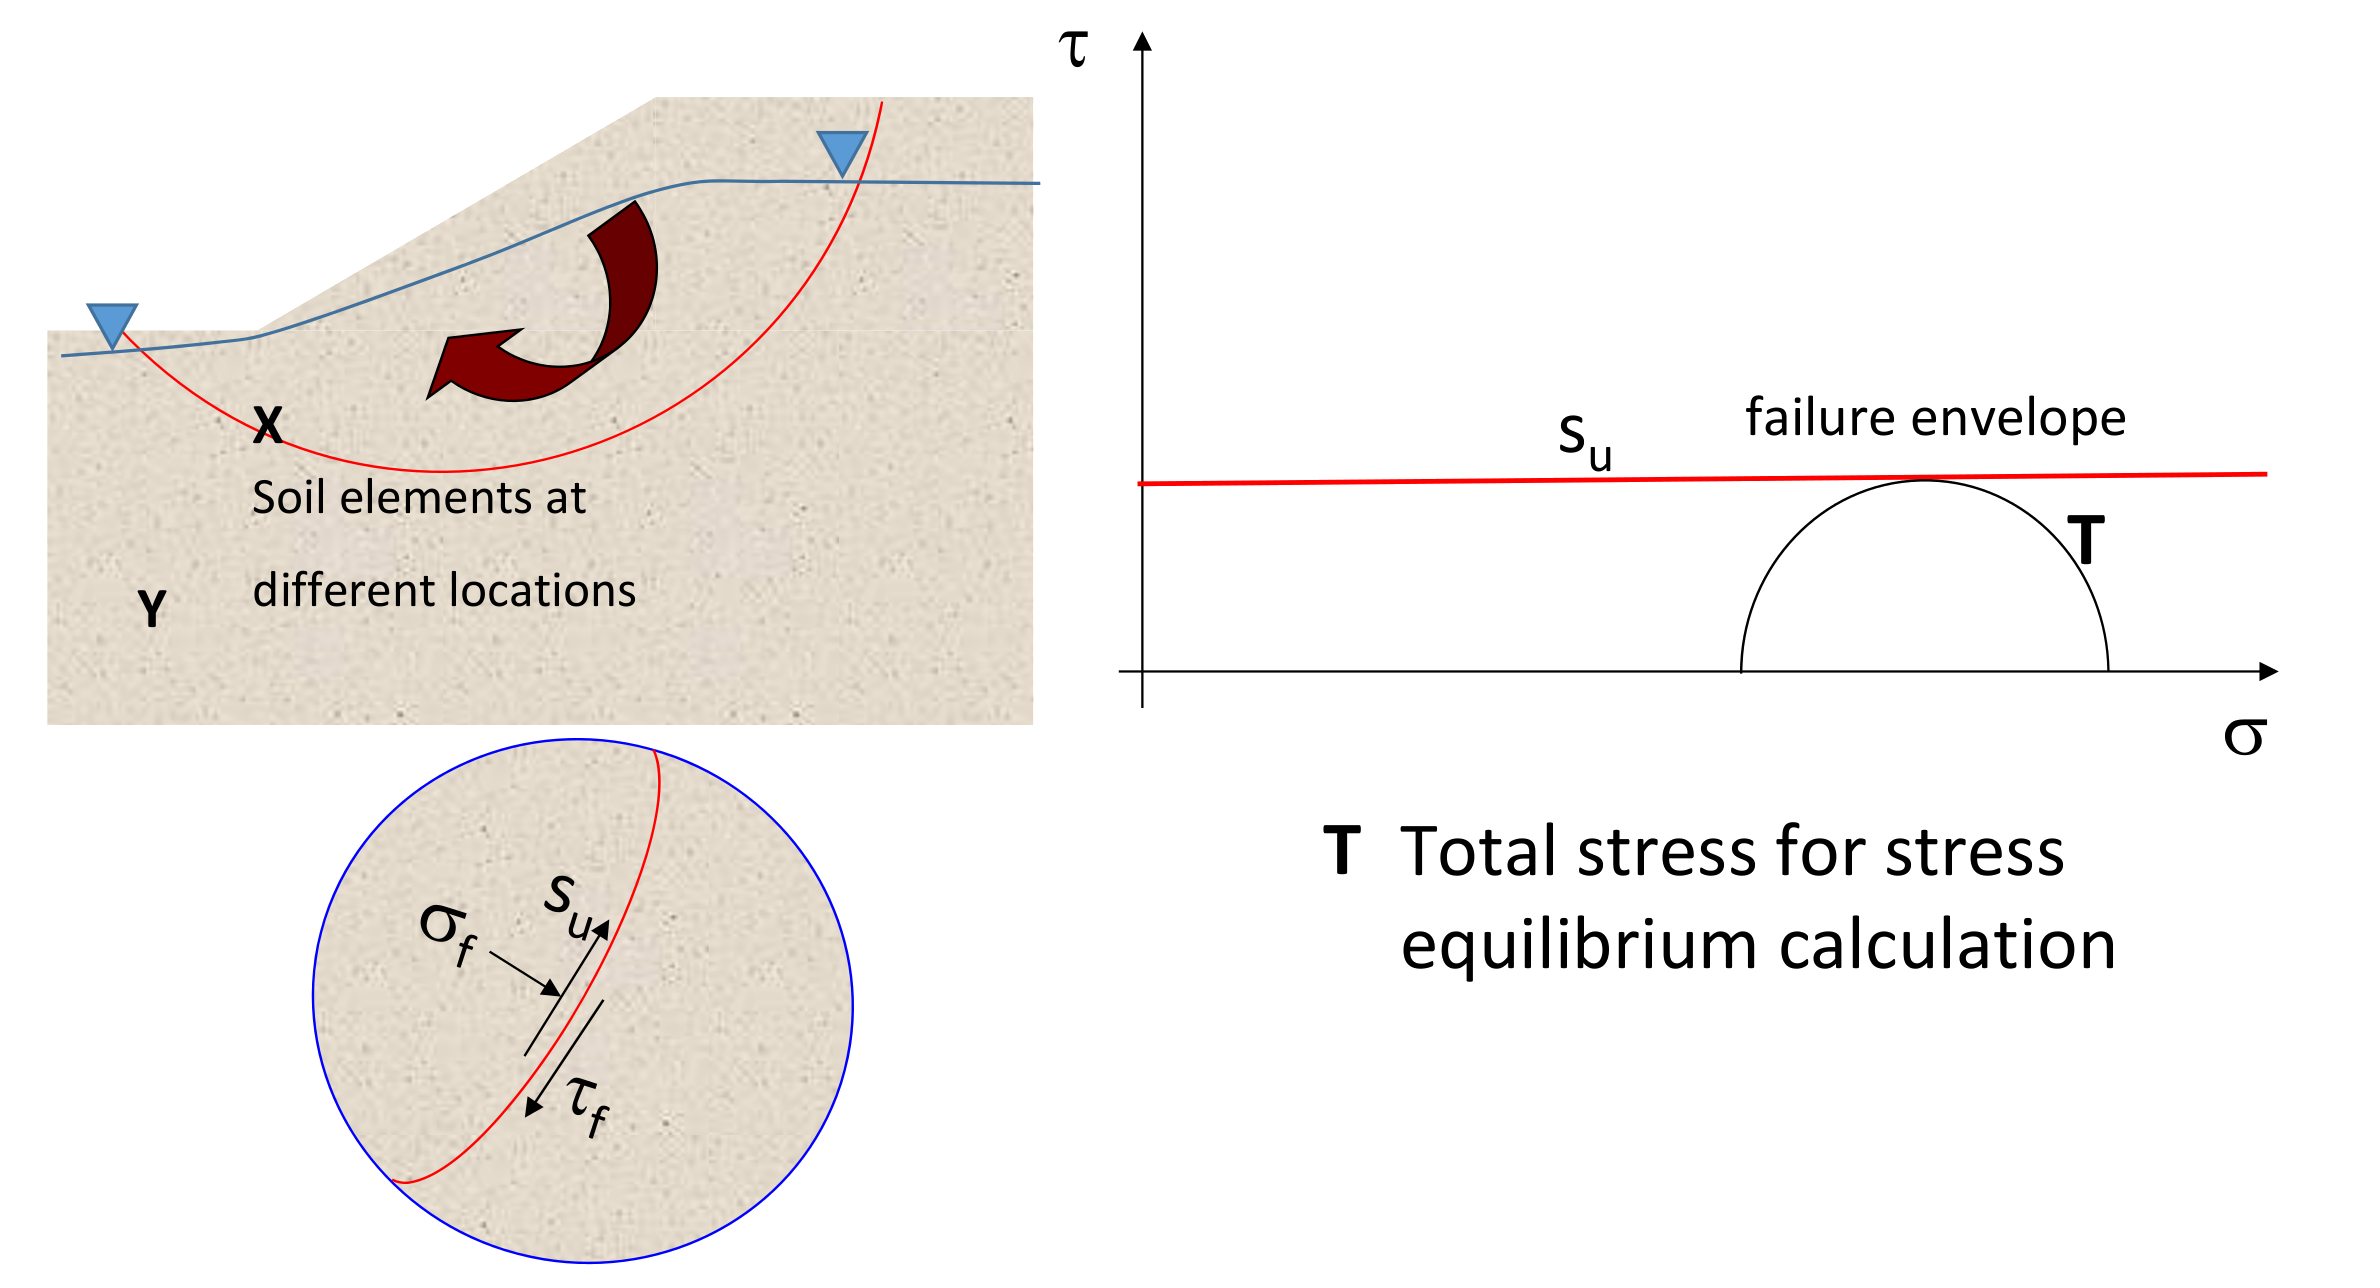
\includegraphics[width=\textwidth]{figs/saturated-undrained.png}
		\end{figure}
	}
	\mode<handout>{
		\begin{figure}[ht]
			\centering
			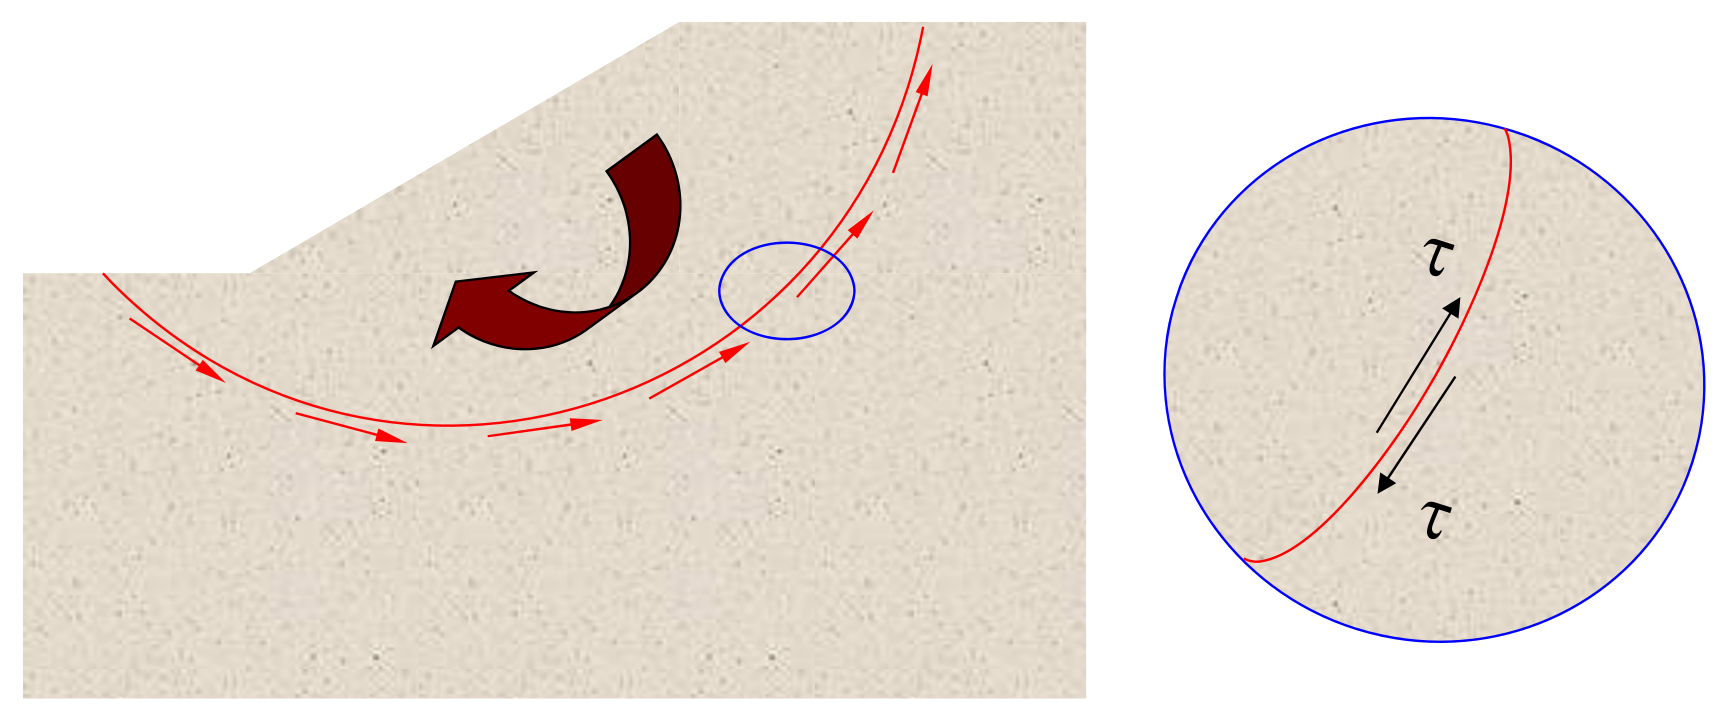
\includegraphics[width=0.9\textwidth]{figs/shear-failure-plane.png}
		\end{figure}
	}
\end{frame}

%------------------------------------------------
\section{Governing equations in stress-deformation analysis}
%------------------------------------------------
\begin{frame}
\frametitle{Governing equations in stress-deformation analysis}
In stress-deformation analysis, we need to consider:
\mode<beamer>{
	\begin{itemize}
		\item \textbf{Equilibrium - static conditions}
		\begin{itemize}
			\item forces and stress must agree across the region of interest. 
			(geometric problem)
		\end{itemize}
		\item \textbf{Compatibility-kinematic conditions}
		\begin{itemize}
			\item geometry, displacement and strains must agree across the
			      region of interest. (geometric problem)
      	\end{itemize}
		\item \textbf{Stress-strain relationship on physical conditions}
		\begin{itemize}
			\item material dependent relationship between stress and strain
			must be specified. (element level)
		\end{itemize}
	\end{itemize}
}
\mode<handout>{
	\vspace{6cm}
}
\end{frame}


%------------------------------------------------
\subsection{Stress equilibrium}
%------------------------------------------------
\begin{frame}
\frametitle{Governing equations in stress-deformation analysis}
The governing differential equation for equilibrium expresses: \mode<beamer>{$\sum \mathbf{F} = m \mathbf{a} $}
\mode<beamer>{
 \noindent
 \fboxsep=0pt
 \noindent
 \begin{minipage}[t]{0.48\linewidth}
	 \begin{itemize}
		\item $\sigma_{xx}$ acting on face $dy$ in the $-x$ direction
		\item $\tau_{xy}$ acting on face $dx$ in the $-x$ direction
		
		\item $\sigma_{xx} + \frac{\partial \sigma_{xx}}{\partial x} dx$ acting on face $dy$ in the $+x$ direction
		
		\item $\tau_{xy} + \frac{\partial \tau_{xy}}{\partial y} dy$ acting on face $dx$ in the $+x$ direction
		
		\item Plus ``body forces'' due to gravity: $\rho f_x dx dy$ where $f_x$ is body force per unit mass
	\end{itemize}
 \end{minipage}%
 \hfill%
 \begin{minipage}[t]{0.48\linewidth}
 	\begin{figure}
 		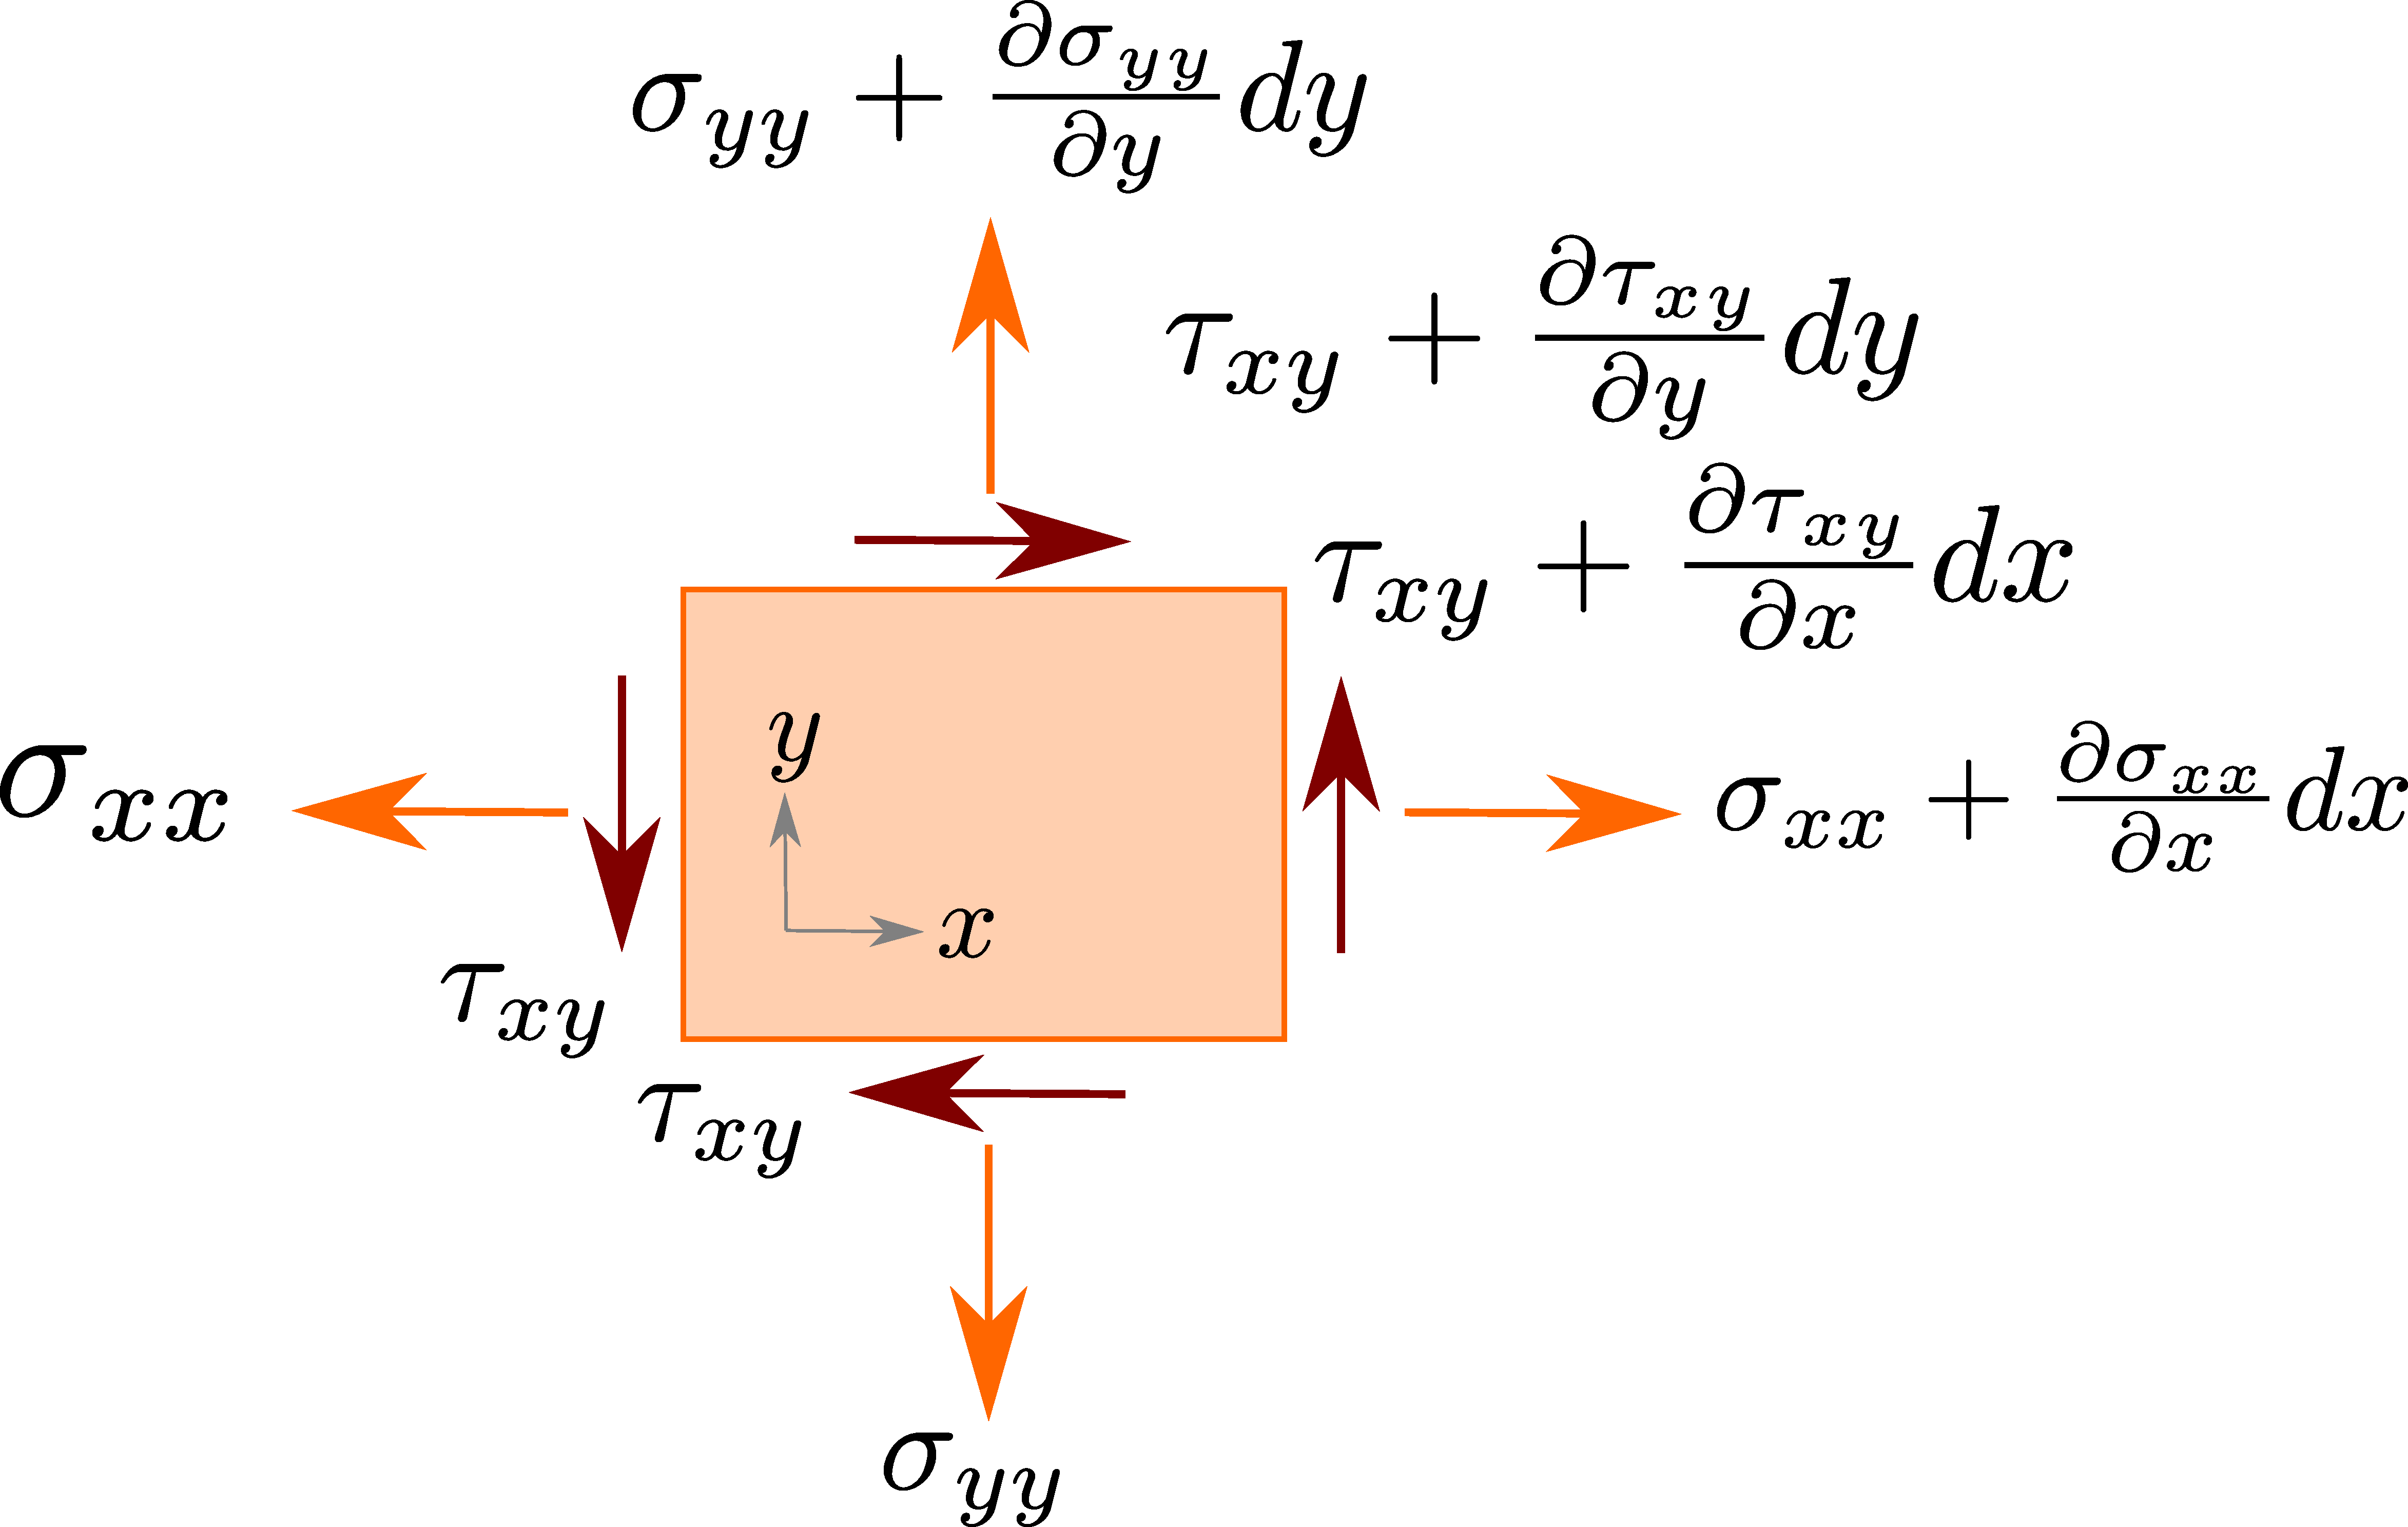
\includegraphics[width=\linewidth]{figs/equilibrium-finished.pdf}
 	\end{figure}
 \end{minipage}
}
\mode<handout>{
 	\begin{figure}
		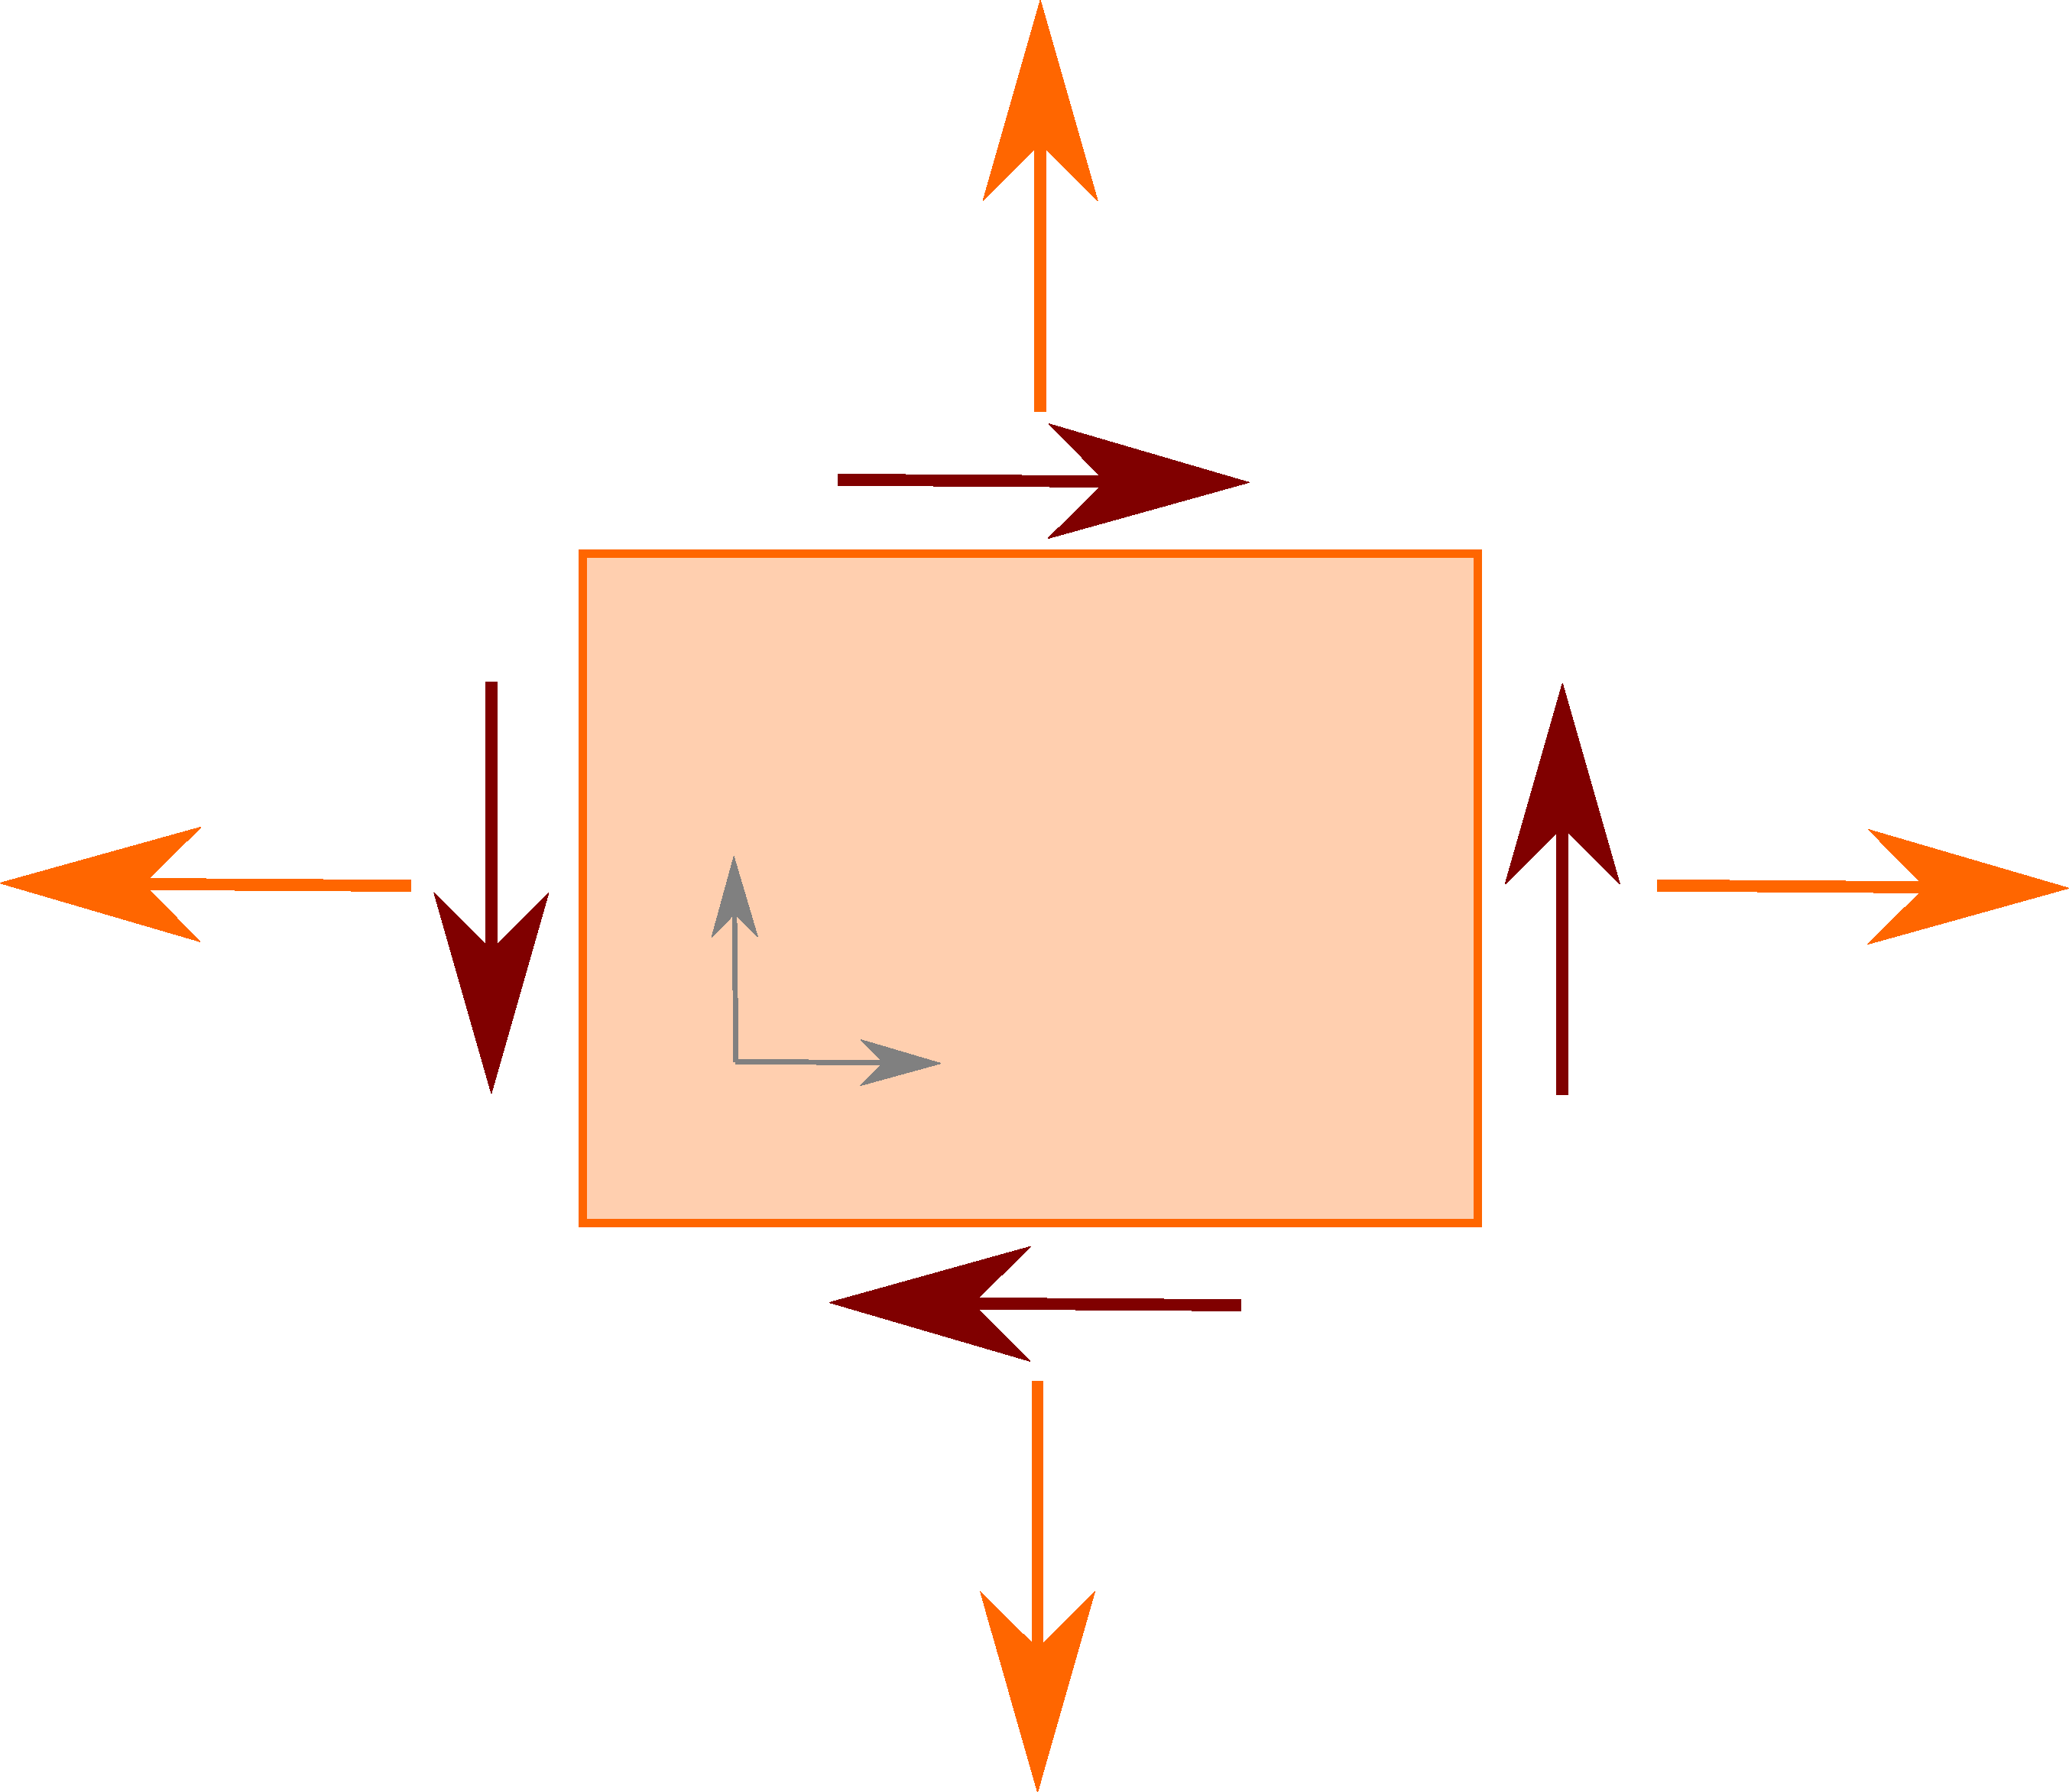
\includegraphics[width=0.6\linewidth]{figs/equilibrium.pdf}
	\end{figure}
}
\end{frame}

\note{
	$\sigma_{xy}$, the term $x$ denotes the direction of the stress component acts on a cut normal to the x-axis (denotes the plane). The $y$ denotes the direction of the stress component.\\
	
	Frequently in the literature the axes are labelled 1, 2 \& 3 rather than x, y \& z.
}
%------------------------------------------------
\begin{frame}
\frametitle{Equilibrium equations}
Summing all this in the x-direction gives:
\mode<beamer>{
	\begin{multline*}
	-\sigma_{xx}dy - \tau_{xy}dx + %
	\left( \sigma_{xx} + \frac{\partial \sigma_{xx}}{\partial x} dx \right) dy \\%
	+ \left( \tau_{xy} + \frac{\partial \tau_{xy}}{\partial y} dy \right) dx + \rho f_x dx dy = %
	\rho dx dy a_x	
	\end{multline*}
}	
\mode<handout>{
	\vspace{2.5cm}
}

Cleaning up terms that cancel, and dividing through by \(dx dy\) gives
\mode<beamer>{
	\begin{equation*}
	\frac{\partial \sigma_{xx}}{\partial x} + %
	\frac{\partial \tau_{xy}}{\partial y}   + \rho f_x = %
	\rho a_x
	\end{equation*}
}	
\mode<handout>{
	\vspace{2cm}
}
	And summing forces in the y-direction leads to:
\mode<beamer>{
	\begin{equation*}	
	\frac{\partial \sigma_{yy}}{\partial y} + %
	\frac{\partial \tau_{xy}}{\partial x}   + \rho f_y = %
	\rho a_y
	\end{equation*}
}	
\mode<handout>{
	\vspace{1.5cm}
}
\end{frame}

%------------------------------------------------
\begin{frame}
\frametitle{Equilibrium in 3D}
 	\begin{figure}
		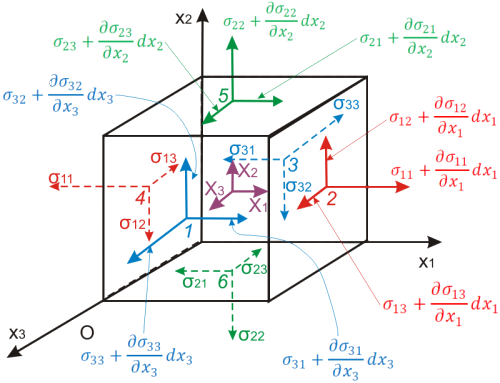
\includegraphics[width=0.8\linewidth]{figs/stress-equilibrium.png}
	\end{figure}
\end{frame}


%------------------------------------------------
\begin{frame}
\frametitle{Equilibrium in 3D}
\mode<beamer>{
	\begin{align*}
	\frac{\partial \sigma_{xx}}{\partial x} +%
	\frac{\partial \sigma_{xy}}{\partial y} +%
	\frac{\partial \sigma_{xz}}{\partial z} + \rho f_x &= \rho a_x \\
	%
	\frac{\partial \sigma_{yx}}{\partial x} +%
	\frac{\partial \sigma_{yy}}{\partial y} +%
	\frac{\partial \sigma_{yz}}{\partial z} + \rho f_y &= \rho a_y \\
	%
	\frac{\partial \sigma_{zx}}{\partial x} +%
	\frac{\partial \sigma_{zy}}{\partial y} +%
	\frac{\partial \sigma_{zz}}{\partial z} + \rho f_z &= \rho a_z \\
	\end{align*}
}	
\mode<handout>{
\vspace{2.5cm}
}
The governing differential equation for equilibrium expresses $\sum \mathbf{F}=m\mathbf{a}$ in terms of derivatives of the stress tensor as:
\mode<beamer>{
$\nabla \cdot \bm{\sigma} + \rho \mathbf{f} = \rho \mathbf{a}$

$\bm{\sigma}$ is the stress tensor, \\
$\rho$ is density, \\
$\mathbf{f}$ is the body force vector per unit mass and \\
$\mathbf{a}$ is the acceleration vector.
}
\end{frame}

%------------------------------------------------
\begin{frame}
\frametitle{Stress equilibrium}
If the object is in equilibrium, then \mode<beamer>{$\mathbf{a}=0$ and $\sum \mathbf{F}=0$.} 

\mode<beamer>{
	\begin{align*}
	\frac{\partial \sigma_{xx}}{\partial x} +%
	\frac{\partial \sigma_{xy}}{\partial y} +%
	\frac{\partial \sigma_{xz}}{\partial z} + b_x &= 0\\
	%
	\frac{\partial \sigma_{yx}}{\partial x} +%
	\frac{\partial \sigma_{yy}}{\partial y} +%
	\frac{\partial \sigma_{yz}}{\partial z} + b_y &= 0\\
	%
	\frac{\partial \sigma_{zx}}{\partial x} +%
	\frac{\partial \sigma_{zy}}{\partial y} +%
	\frac{\partial \sigma_{zz}}{\partial z} + b_z &= 0\\
	\end{align*}
}	
\mode<handout>{
	\vspace{2.5cm}
}
Stresses: \mode<beamer>{$\left[\sigma_{xx}, \sigma_{yy}, \sigma_{zz}, \sigma_{xy}, \sigma_{yz}, \sigma_{zx}\right]^T$.}

Equilibrium equation: \mode<beamer>{$\nabla^T \bm{\sigma} + \mathbf{b} = 0$}

Then: \mode<beamer>{
	\begin{equation*}
	\nabla^T = %
	\begin{bmatrix}
	\frac{\partial}{\partial x} & 0 & 0 & \frac{\partial}{\partial y} & 0 & \frac{\partial}{\partial z} \\
	0 & \frac{\partial}{\partial y} & 0 & \frac{\partial}{\partial x} & \frac{\partial}{\partial z} & 0 \\
	0 & 0 & \frac{\partial}{\partial z} & 0 & \frac{\partial}{\partial y} & \frac{\partial}{\partial x}
	\end{bmatrix}
	\end{equation*}
}
\end{frame}

\note{
	Divergence is a vector operator that produces a scalar field, giving the quantity of a vector 
	field's source at each point. In physical terms, the extent to which there is more of some 
	quantity exiting an infinitesimal region of space than entering it. If the divergence is nonzero 
	at some point then there is compression or expansion at that point. 
}
%------------------------------------------------
\subsection{Compatibility condition}
%------------------------------------------------
\begin{frame}
	\frametitle{Compatibility}
	\mode<handout>{\vspace{4cm}}
	\mode<beamer>{
		\begin{itemize}
			\item compatibility relates the deformations of a structure so that its
			various parts (members, joints, and supports) fit together without any gaps or
			overlaps. 
			\item ensure that the deformed shape of the structure is continuous (except at the 
			locations of any internal hinges or rollers), and is consistent with the support
			conditions.
		\end{itemize}
	}
\end{frame}


%------------------------------------------------
\begin{frame}
\frametitle{Governing equations: Compatibility}
 	\begin{figure}
	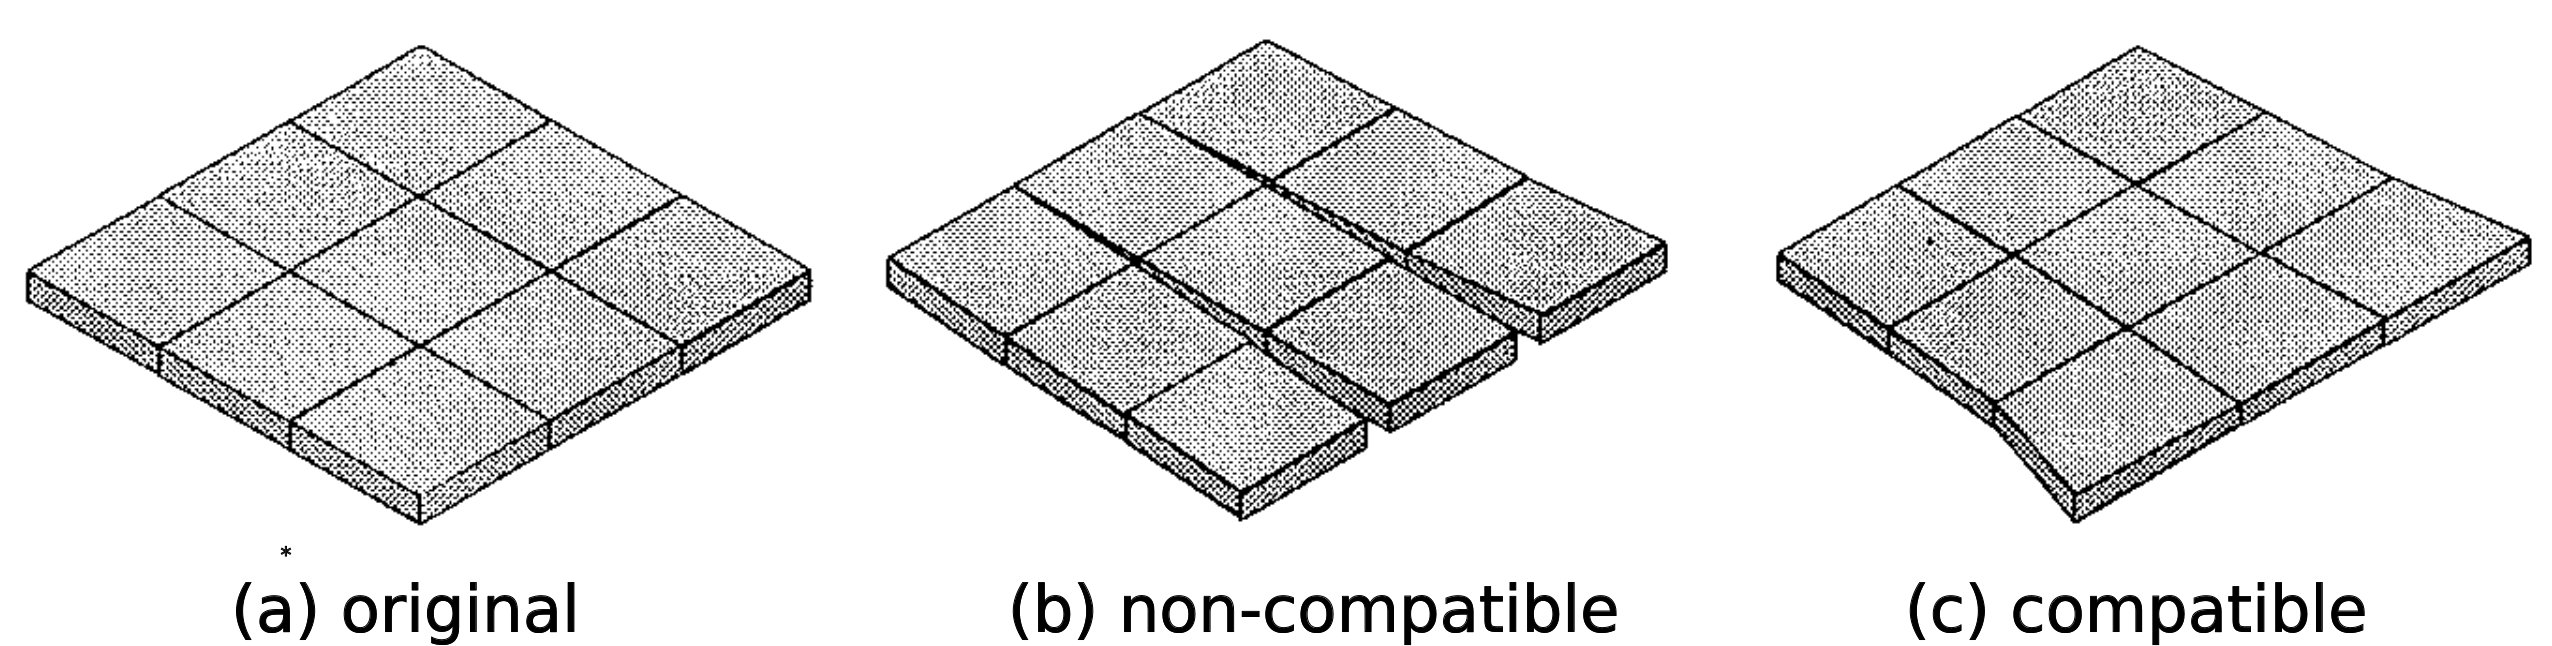
\includegraphics[width=\linewidth]{figs/compatibility.png}
\end{figure}
\end{frame}


%------------------------------------------------
\begin{frame}
\frametitle{Governing equations: Displacement - strain relationship}
Displacement - strain relationship: \mode<beamer>{$\bm\varepsilon = \nabla \mathbf{u}$}
\noindent
\fboxsep=0pt
\noindent
\begin{minipage}[t]{0.48\linewidth}
	\mode<beamer>{
		Where,
		\begin{align*}
		\varepsilon_{xx} & = \frac{\partial u_x}{\partial x}	\\
		\varepsilon_{yy} & = \frac{\partial u_y}{\partial y}	\\
		\gamma_{xy} & = \frac{\partial u_x}{\partial y} + \frac{\partial u_y}{\partial x}	\\
		\end{align*}
		
		\begin{equation*}
			\frac{\partial^2\varepsilon_{xx}}{\partial y^2} + \frac{\partial^2 \varepsilon_{yy}}{\partial x^2} = \frac{\partial^2 \gamma_{xy}}{\partial x \partial y}
		\end{equation*}
	}
	\mode<handout>{
		\vspace{5cm}
	}
\end{minipage}%
\hfill%
\begin{minipage}[t]{0.48\linewidth}
	\begin{figure}
		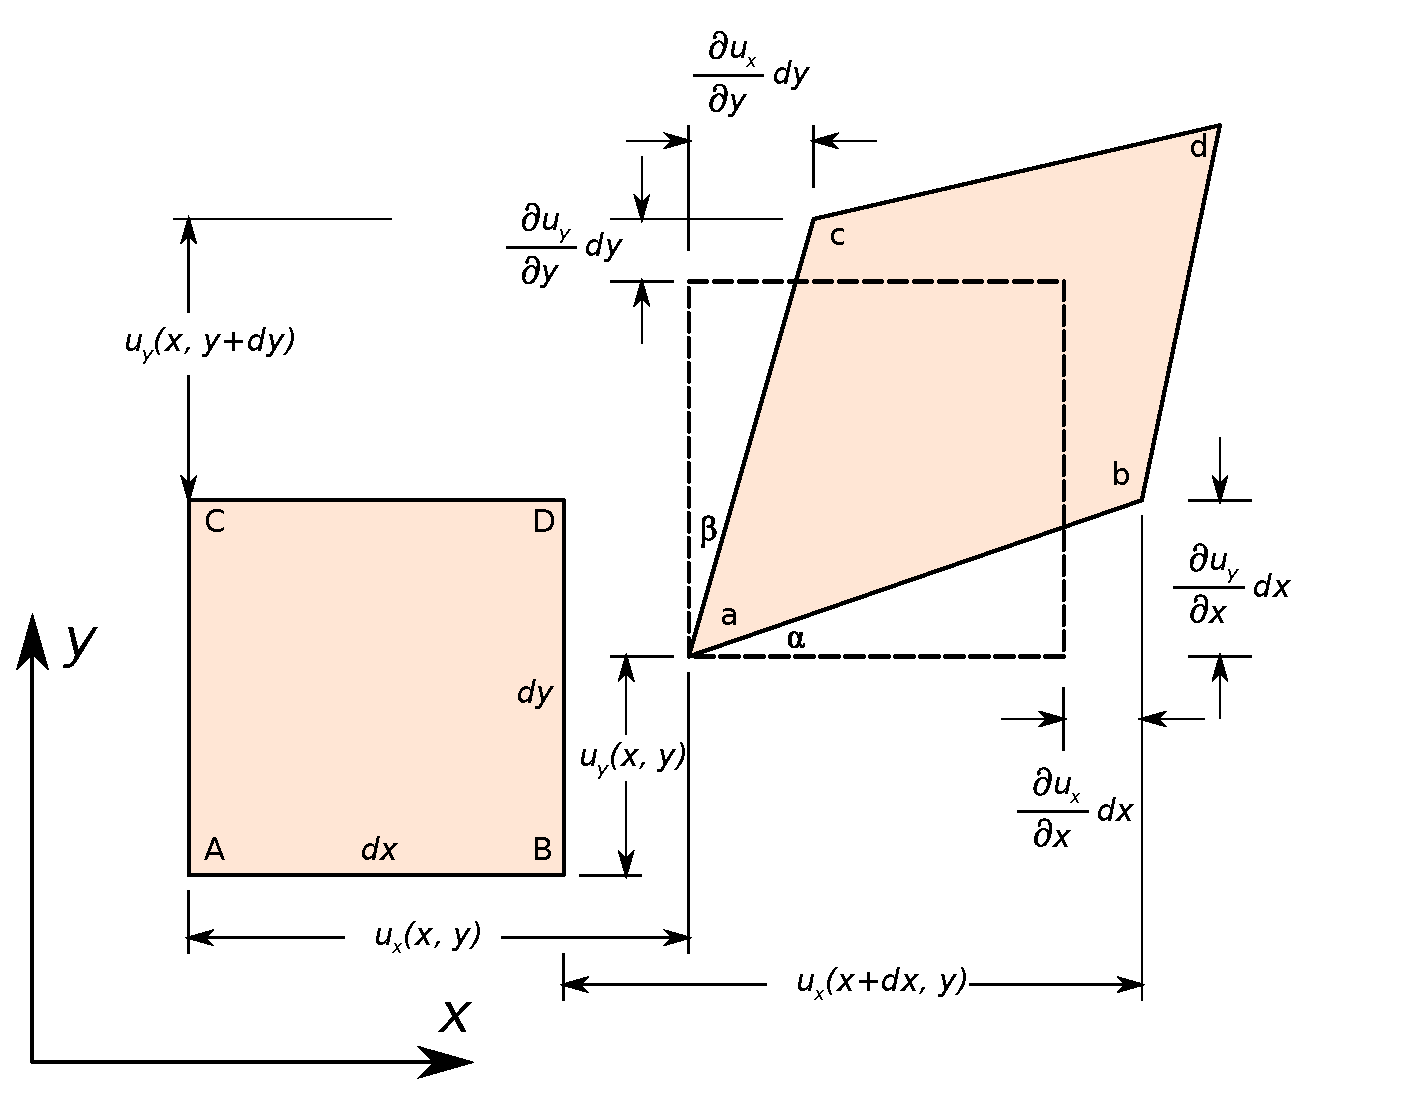
\includegraphics[width=\linewidth]{figs/geometric-strain.pdf}
	\end{figure}
	\mode<beamer>{
		\begin{equation*}
		\varepsilon_{xy} = \frac{\gamma_{xy}}{2} = \frac{1}{2} \left( \frac{\partial u_x}{\partial y} + \frac{\partial u_y}{\partial x} \right)
		\end{equation*}
	}
	\mode<handout>{
		\vspace{2cm}
	}
\end{minipage}%
\end{frame}

\note{
	\textbf{Compatibility in 3D}
	\begin{figure}
		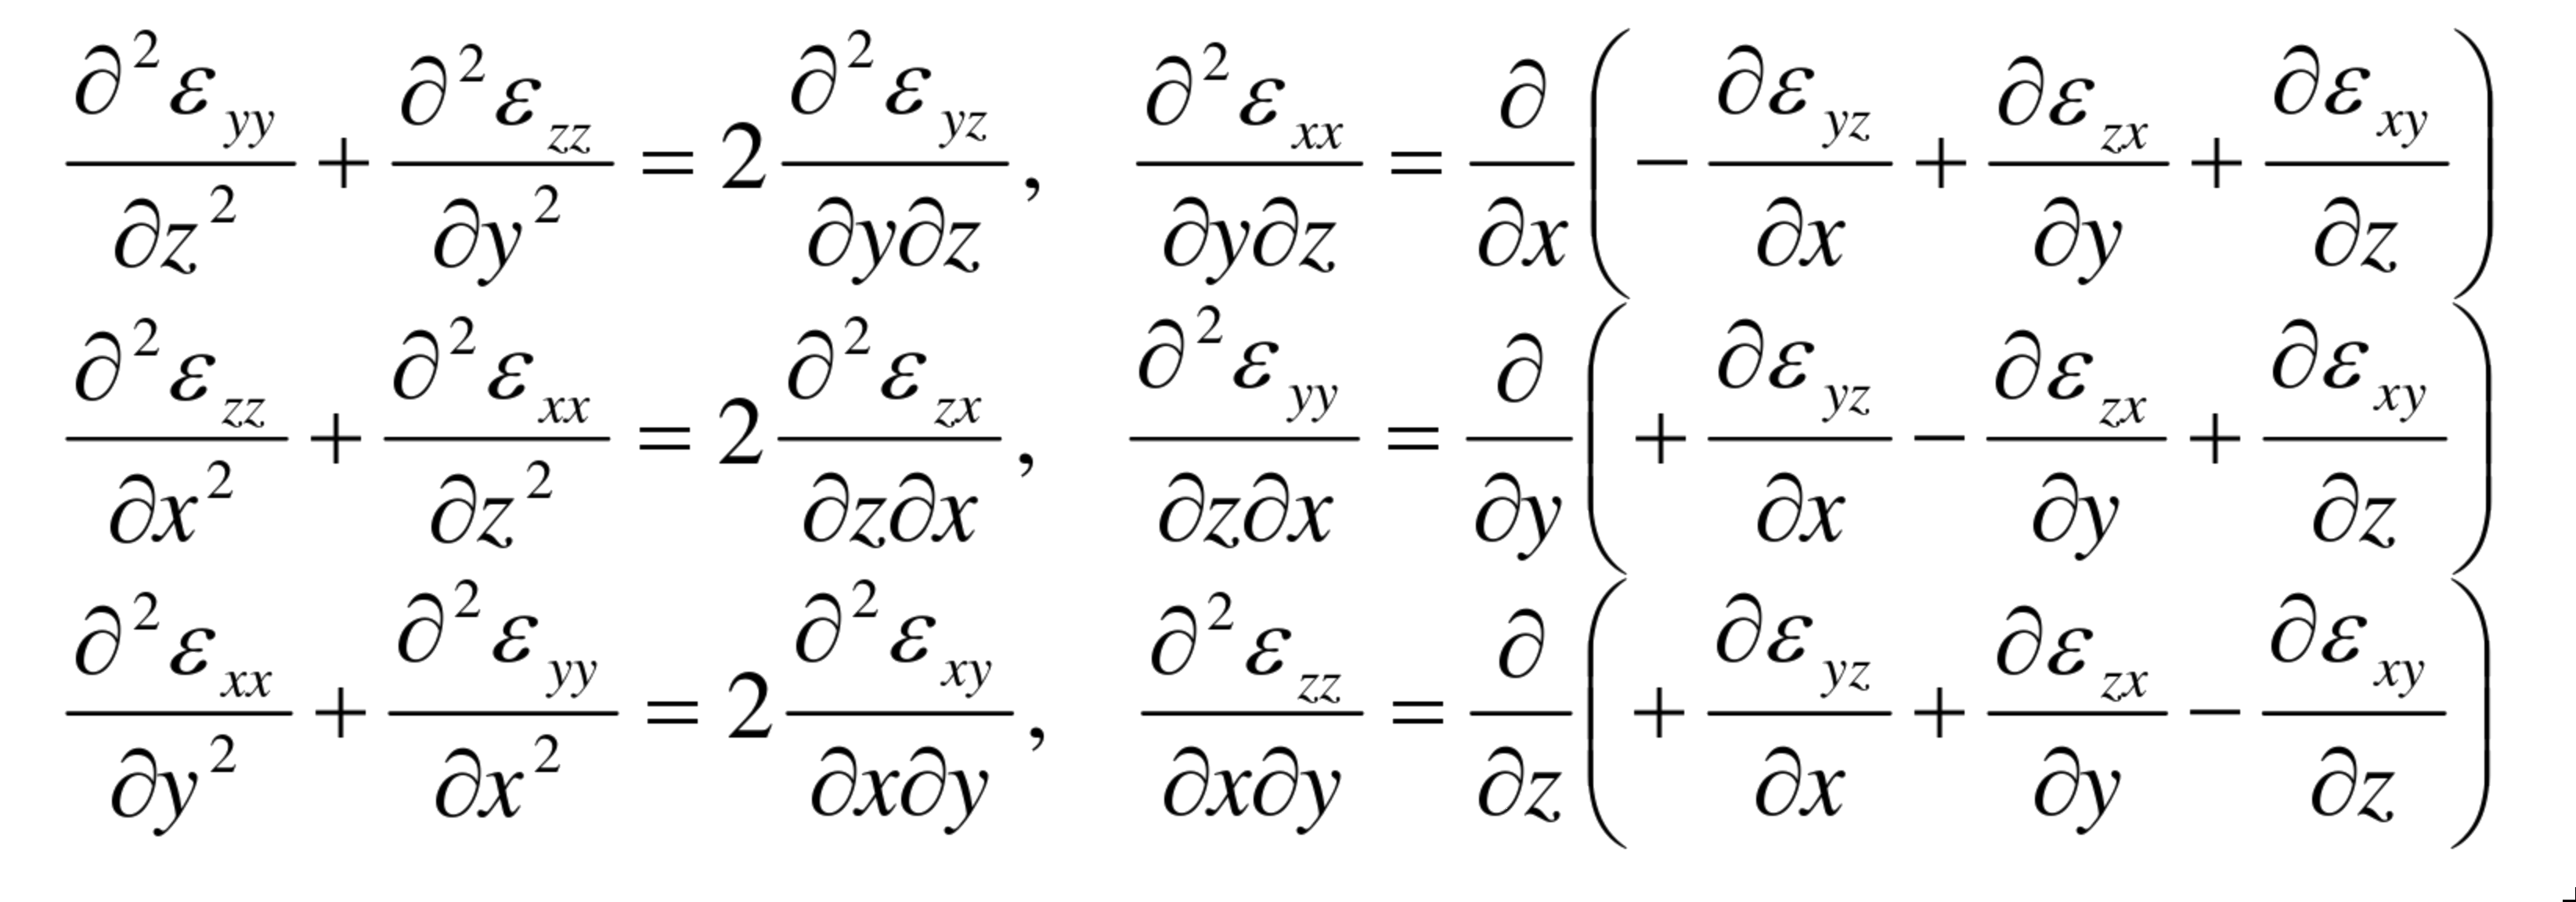
\includegraphics[width=0.85\textwidth]{figs/compatibility-3d.png}
	\end{figure}
}

%------------------------------------------------
\subsection{Stress-strain relationship}
%------------------------------------------------
\begin{frame}
\frametitle{Equilibrium and compatibility conditions}
Combining the Equilibrium and Compatibility conditions gives:
\begin{itemize}
	\item Unknowns: \mode<beamer>{6 stresses + 6 strains + 3 displacements = 15}
	\item Equations:  \mode<beamer>{3 equilibrium + 6 compatibility = 9}
\end{itemize}
\mode<beamer>{To obtain a solution therefore requires 6 more equations. These come from the
constitutive relationships}
\mode<handout>{
	\vspace{2cm}
}
\end{frame}

\begin{frame}
\frametitle{Governing equations: Stress-strain relationship}
Stress - strain relationship: \mode<beamer>{$\bm \sigma = \mathbf{D} \bm\varepsilon$}

\begin{equation*}
	\begin{bmatrix}
	\sigma_{xx} \\
	\sigma_{yy} \\
	\sigma_{zz} \\
	\sigma_{xy} \\
	\sigma_{yz} \\
	\sigma_{zx} \\
	\end{bmatrix} %
	= %
	\mathbf{D (6x6)} %
	\begin{bmatrix}
	\varepsilon_{xx} \\
	\varepsilon_{yy} \\
	\varepsilon_{zz} \\
	\varepsilon_{xy} \\
	\varepsilon_{yz} \\
	\varepsilon_{zx} \\
	\end{bmatrix}
\end{equation*}
\end{frame}

%------------------------------------------------
\begin{frame}
\frametitle{Governing equations in stress-deformation analysis}
What are the variables used in the governing equations?
\mode<beamer>{
	\begin{enumerate}
		\item displacements $\mathbf{u}$ in the body
		\item strains $\bm\varepsilon$ in the body or within the elements
		\item stresses $\bm\sigma$ in the body or within the elements
	\end{enumerate}
}	
\mode<handout>{
\vspace{2.5cm}
}
Advanced analysis involves:
\mode<beamer>{
	\begin{enumerate}
		\item Equilibrium: External forces + internal stresses agree
		\item Compatibility: Displacements fields agree (no gaps) + strains (derivatives)
		\item Stress-strain relationship (constitutive behaviour)
	\end{enumerate}
}	
\mode<handout>{
	\vspace{2.5cm}
}
\end{frame}

\section{Limit analysis}
%------------------------------------------------
\begin{frame}
	\frametitle{Limit analysis: Lower and upper bound theorems}
	The exact determination of loads involved in the plastic deformation requires simultaneous solution of three sets of conditions:
	\begin{enumerate}
		\item equations of equilibrium
		\item equations of compatibility
		\item appropriate constitutive criteria (yield condition and flow rule)
	\end{enumerate}
	
	Exact determination is often not easy, may be appropriate for simple shapes, but other cases we may have to use \textit{numerical method}.
\end{frame}

\note{Calculations of slope stability are based on plasticity theory, which is held
	to be applicable to ductile materials such as soils. Strictly, plasticity theory
	applies only to perfectly plastic materials that adhere to the normality
	principle, which maximises the work done in plastic deformations.}

%------------------------------------------------
\begin{frame}
	\frametitle{Limit analysis: Lower bound theorem}
	
	``\textit{If there is a set of external loads \textbf{which are in equilibrium} with a state of
 stress that nowhere exceeds the failure criterion for the material, \textbf{collapse cannot occur} and the external loads are a lower bound to the true
	collapse loads}''\\
	\vspace{1em}
	
	Any applied load is less than the actual limiting load, i.e., they will not cause collapse.\\
	\mode<beamer>{
	\begin{enumerate}
		\item satisfies equilibrium everywhere
		\item balances the externally applied loads, and
		\item every point is within the yield locus.
	\end{enumerate}
	\textbf{Relax compatibility.}
	}\mode<handout>{
	\vspace{5cm}
	}
\end{frame}

%------------------------------------------------
\begin{frame}
	\frametitle{Lower bound solution}
	We need to determine a set of
stresses in the ground that are in equilibrium with the external
loads. Stress state everywhere should be:
	\mode<beamer>{
		\centering
		$\sigma_1 - \sigma_3 = s_u$
		\begin{figure}
			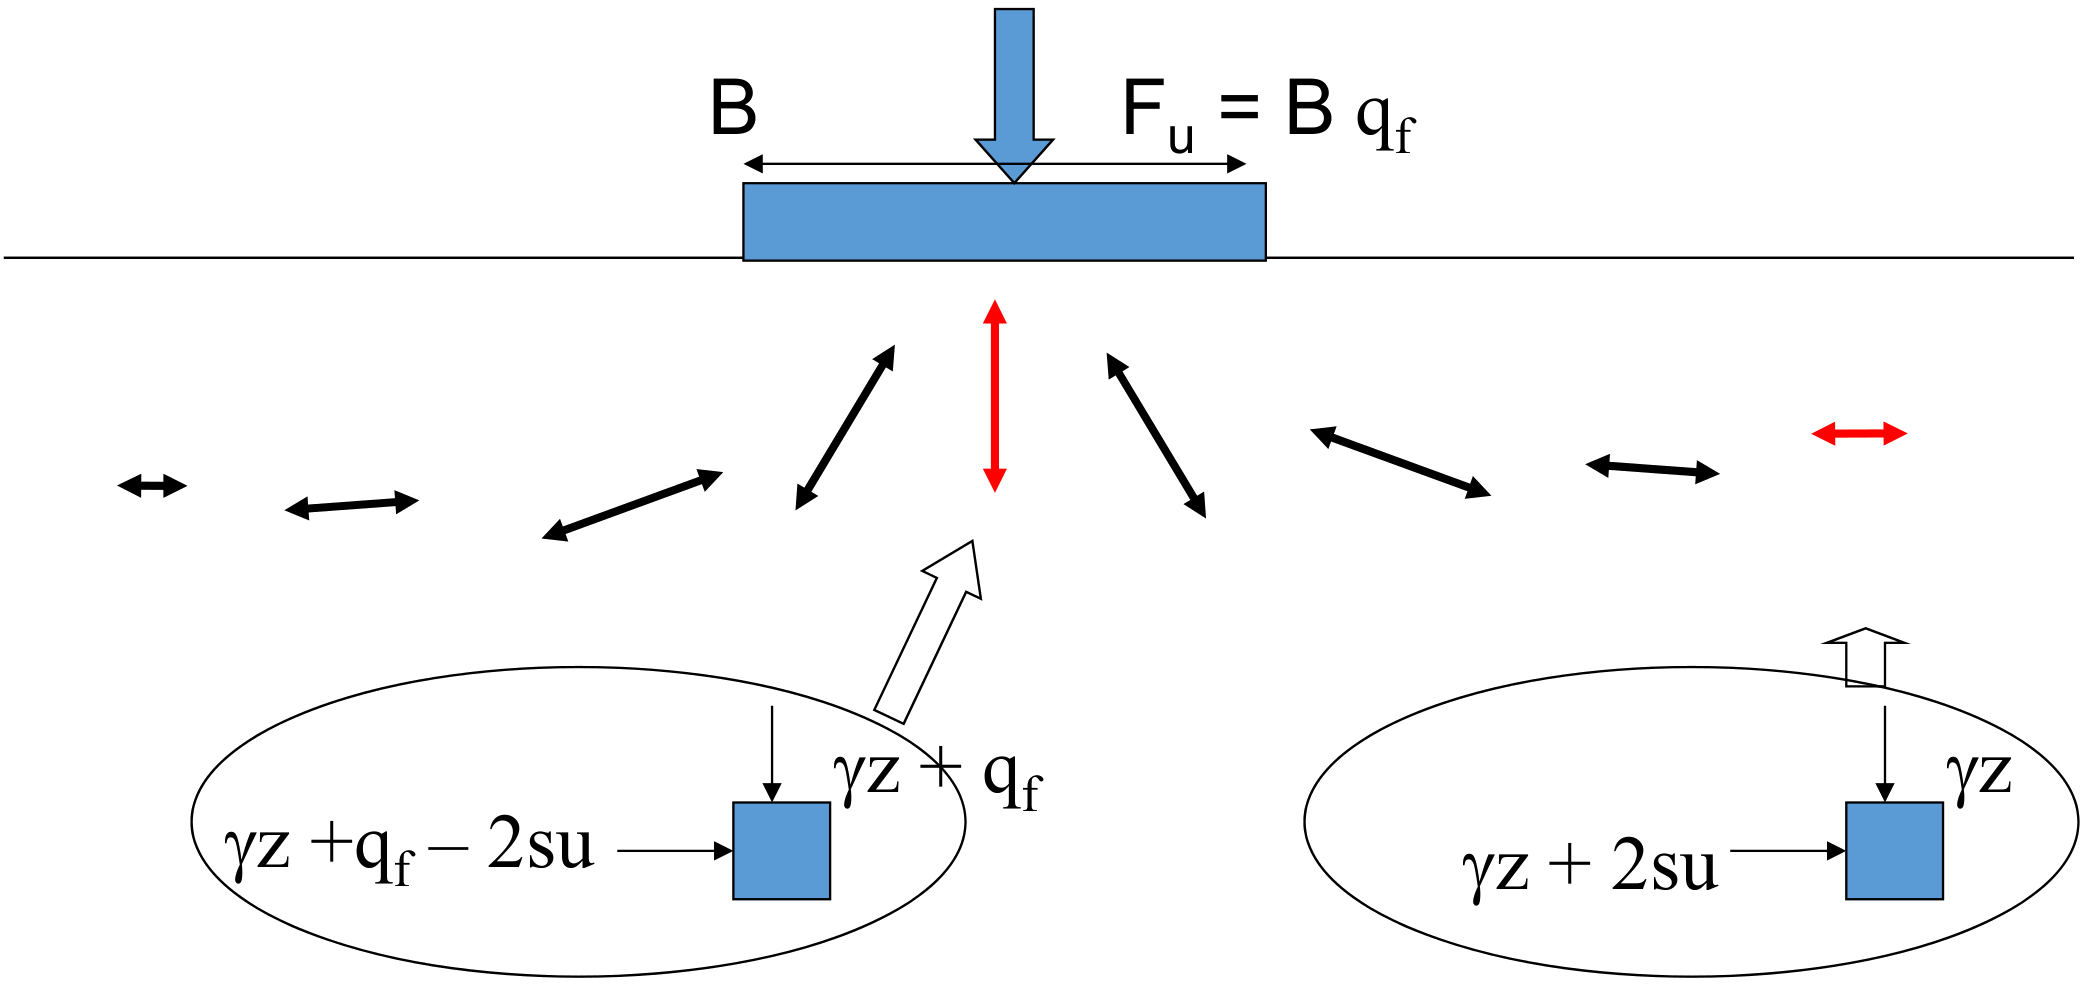
\includegraphics[width=0.85\linewidth]{figs/lb-foundation.png}
		\end{figure}
	}\mode<handout>{
		\vspace{5cm}
	}
\end{frame}

%------------------------------------------------
\begin{frame}
	\frametitle{Limit analysis: Upper bound theorem}
	``\textit{If there is a set of external loads and a mechanism of plastic collapse such
that the increment of work done by the external loads in an \textbf{increment of
	displacement} equals the work done by the internal stresses, \textbf{collapse
must occur} and the external loads are an upper bound to the true
collapse loads}''\\
	\vspace{1em}

	Apply enough load to achieve the desired change in component shape, e.g., process machinery.
	\mode<beamer>{
		\begin{enumerate}
			\item satisfies the boundary displacement conditions, and
			\item do not infringe incompressibility.
		\end{enumerate}
	
	\textbf{Relax equilibrium}
	}\mode<handout>{
	\vspace{5cm}
}
\end{frame}

%------------------------------------------------
\begin{frame}
	\frametitle{Upper bound solution}
	We need to determine a failure
mechanism, which is kinematically feasible. The work done is
equated by the plastic dissipation along the failure (or slip)
	surfaces.
	\mode<beamer>{
		\begin{figure}
			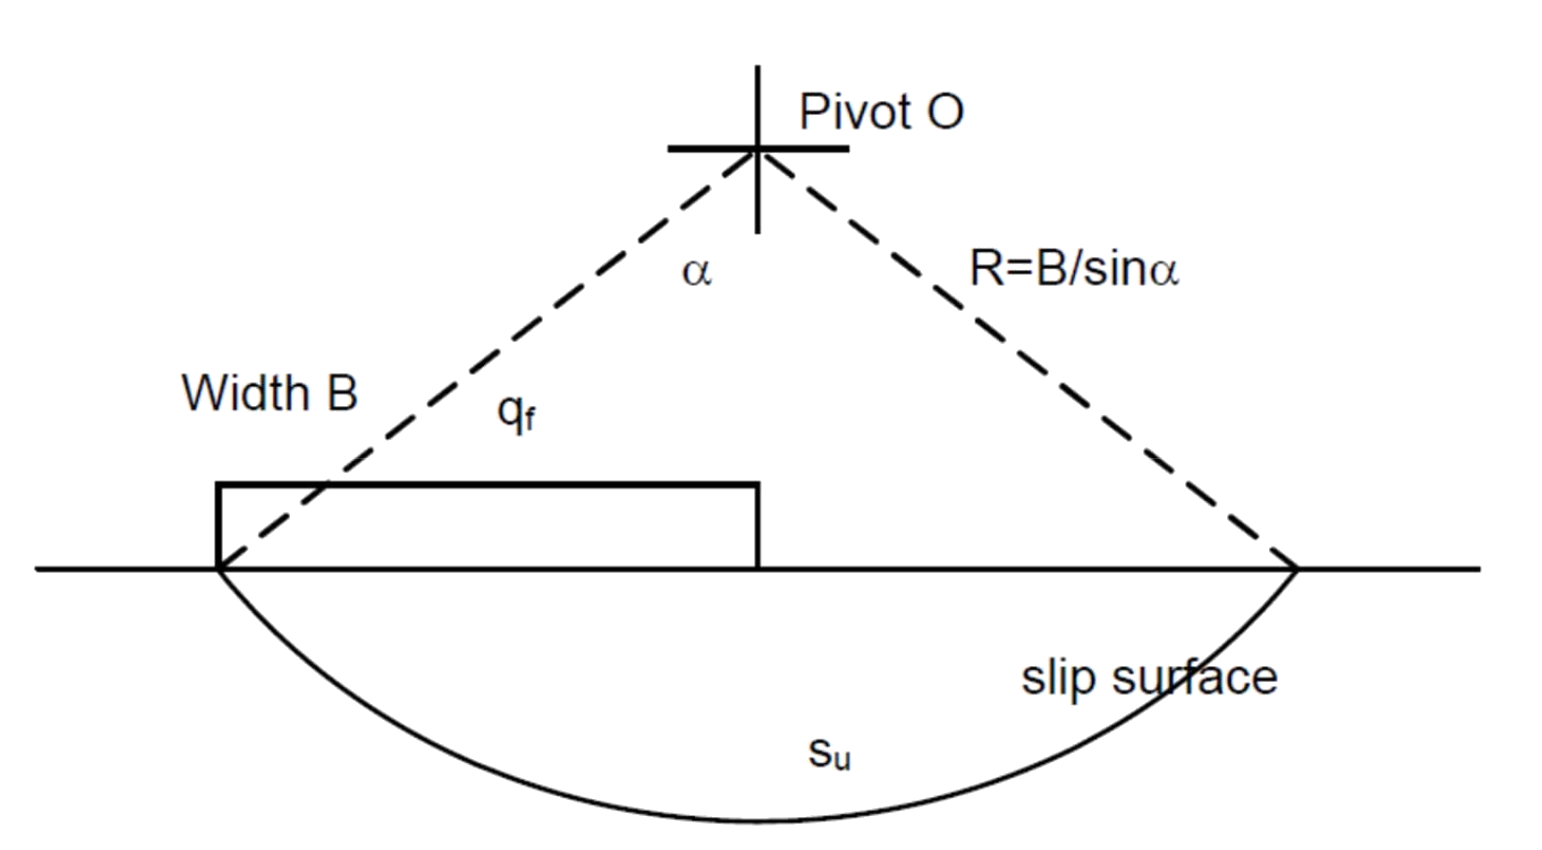
\includegraphics[width=0.7\linewidth]{figs/ub-foundation.png}
		\end{figure}
	}
\mode<handout>{
	\vspace{5cm}
}
\end{frame}

\note{Exact solution is between upper and lower bound.}

%------------------------------------------------
\begin{frame}
	\frametitle{Undrained cut: Lower bound solution}
	Consider the equilibrium of an element of soil adjacent to the bottom of a cut, or
	crack. Assume that the major principal stress is vertical, and that the soil fails
	according to Tresca’s criterion at a shear stress $s_u$ (undrained strength).
	\mode<beamer>{
		\begin{figure}
			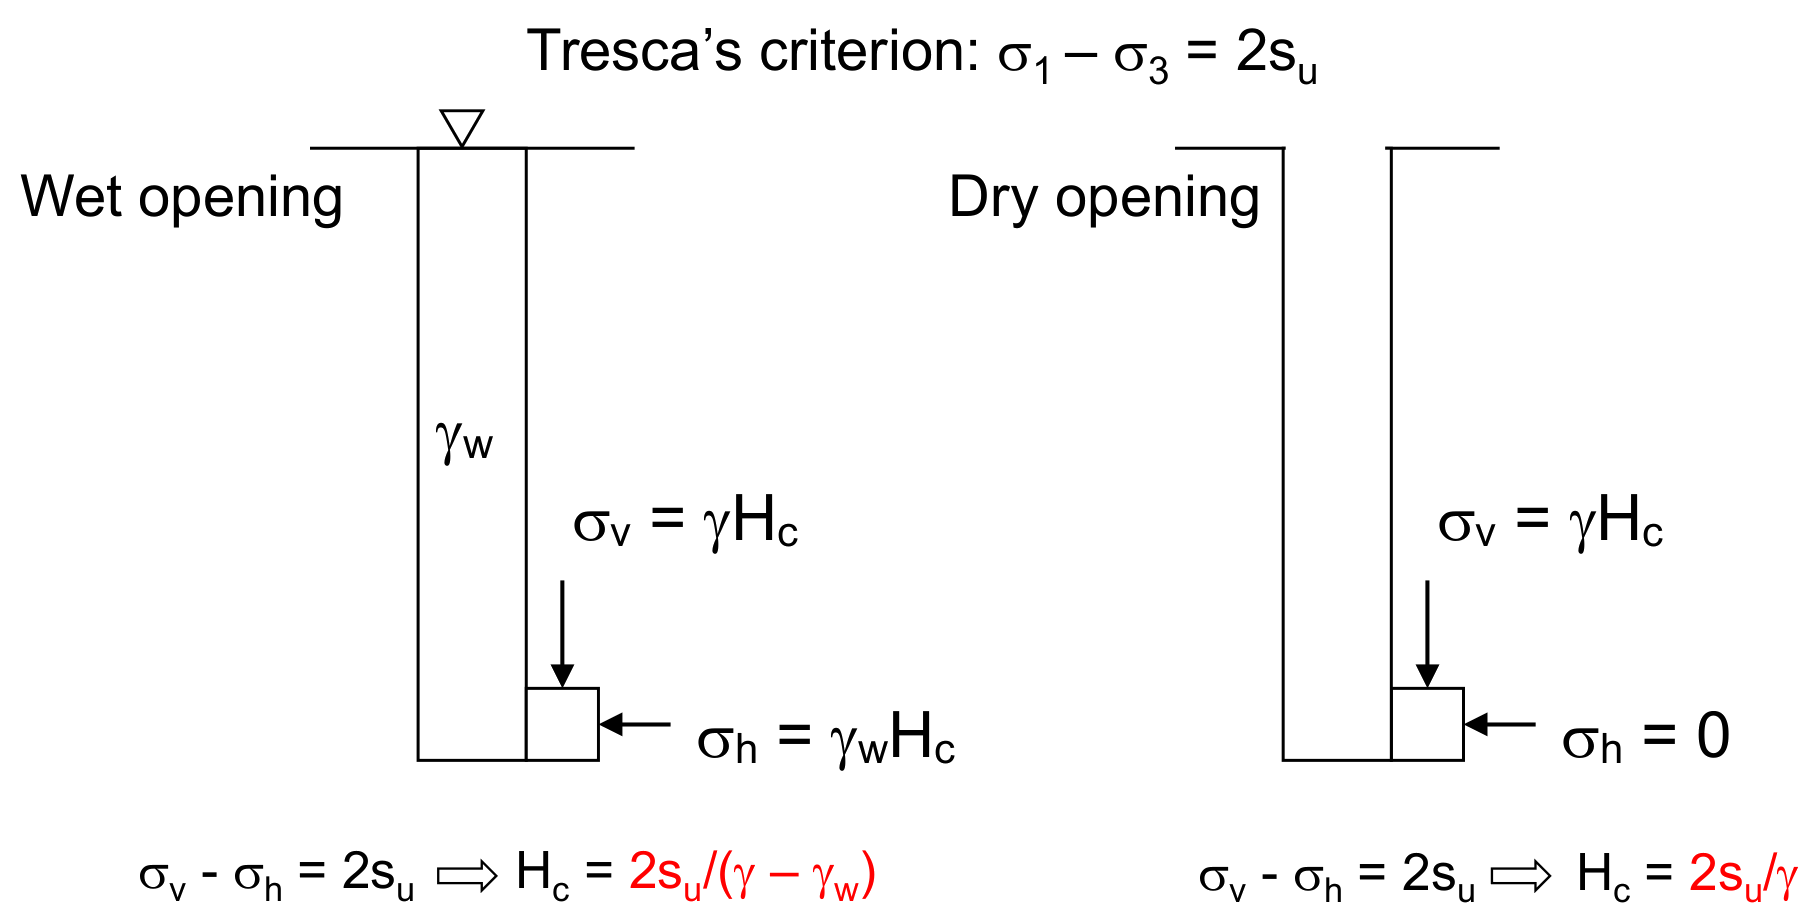
\includegraphics[width=0.8\linewidth]{figs/lb-vertical-cut.png}
		\end{figure}
	
	The resulting maximum depth of crack, $H_c$, is different in wet and dry conditions.
	A deeper crack can be kept open if it fills with water.
	}
\mode<handout>{
	\vspace{5cm}
}
\end{frame}


%------------------------------------------------
\begin{frame}
	\frametitle{Undrained cut: Upper bound solution - wedge mechanism}
	\mode<beamer>{
	\begin{figure}
		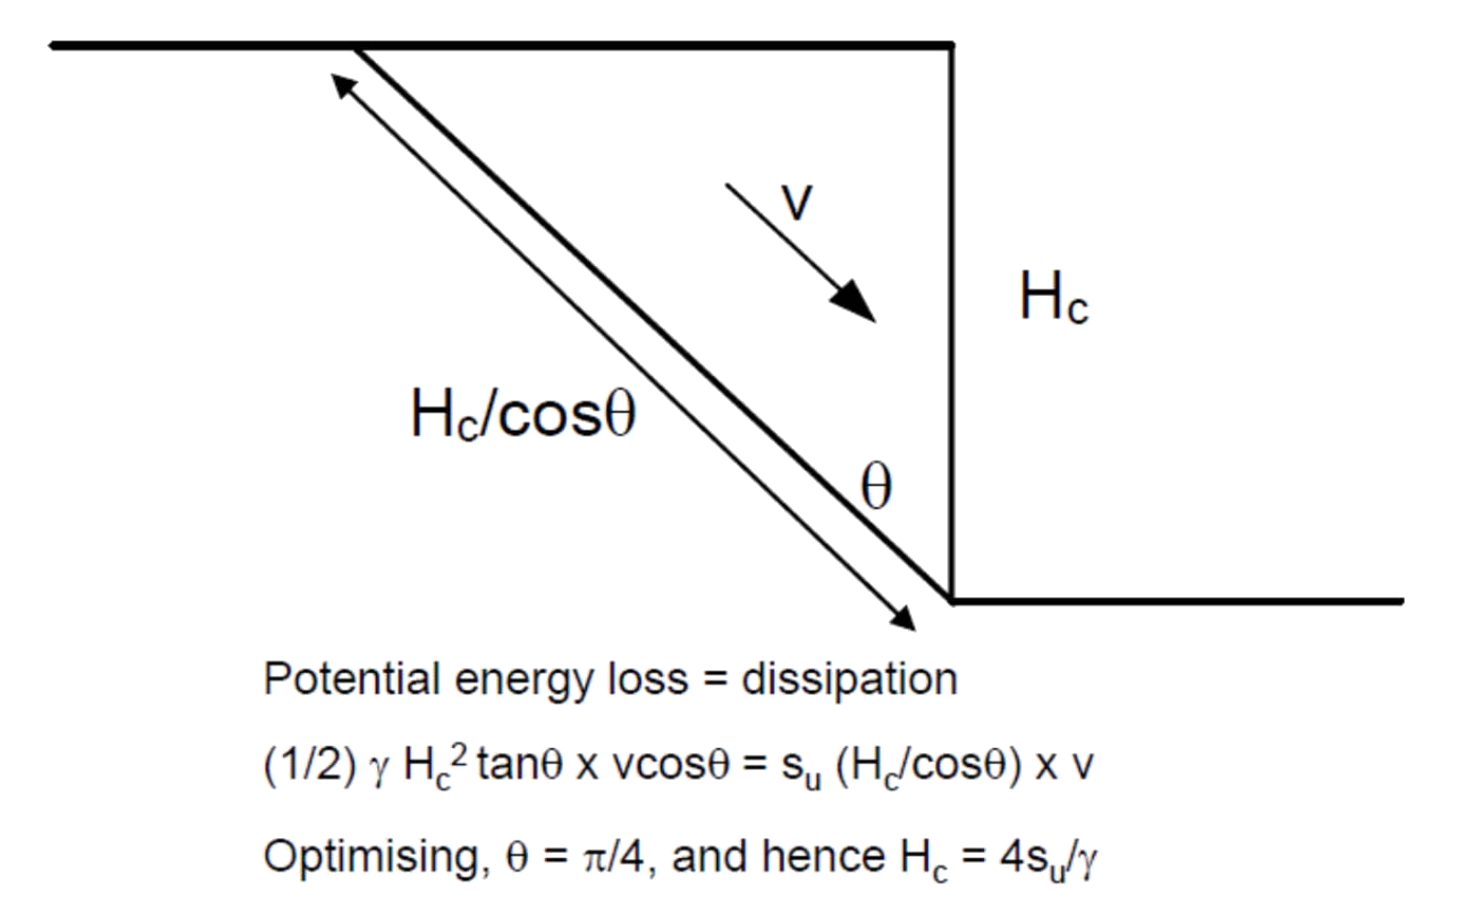
\includegraphics[width=0.8\linewidth]{figs/ub-cut-1.png}
	\end{figure}
	}
	\mode<handout>{
	\begin{figure}
		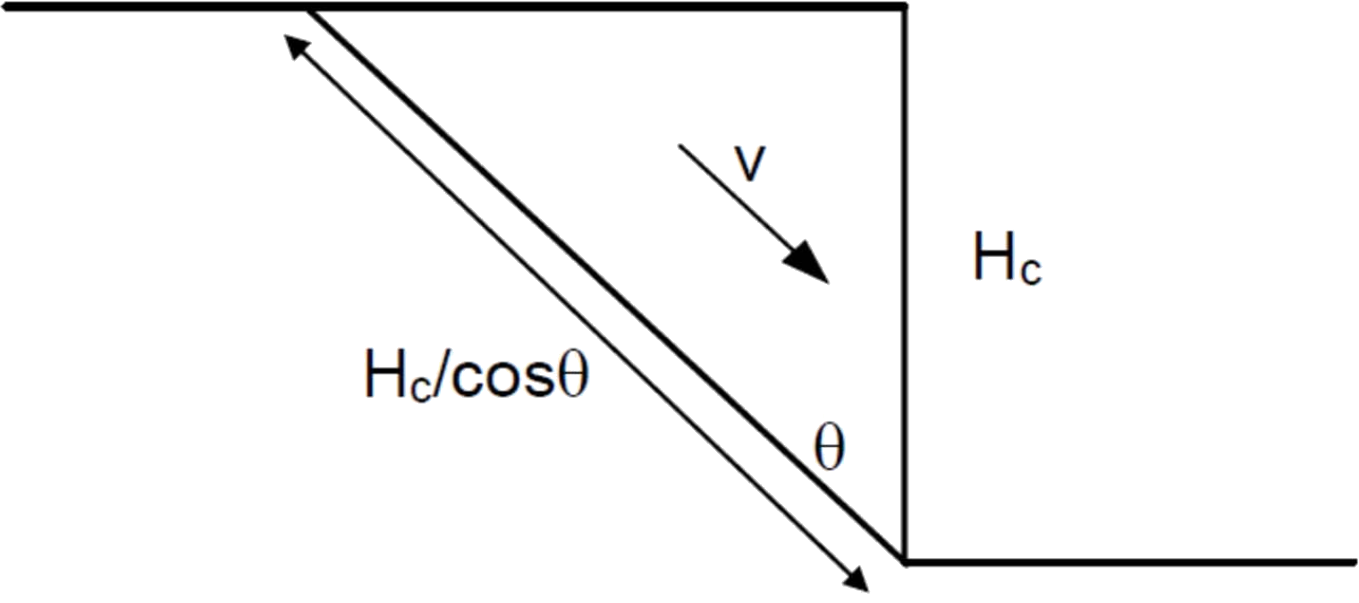
\includegraphics[width=0.8\linewidth]{figs/ub-cut-1-empty.png}
	\end{figure}
    \vspace{2cm}
	}
This simple upper bound solution involving a single sliding block gives a
normalized cut depth, $N_s = \gamma H_c /s_u = 4$. A more refined upper bound solution
involves a circular slip surface, passing through the base of the cut.
	
\end{frame}

%------------------------------------------------
\begin{frame}
	\frametitle{Undrained cut: Upper bound solution - slip circle}
	\begin{figure}
		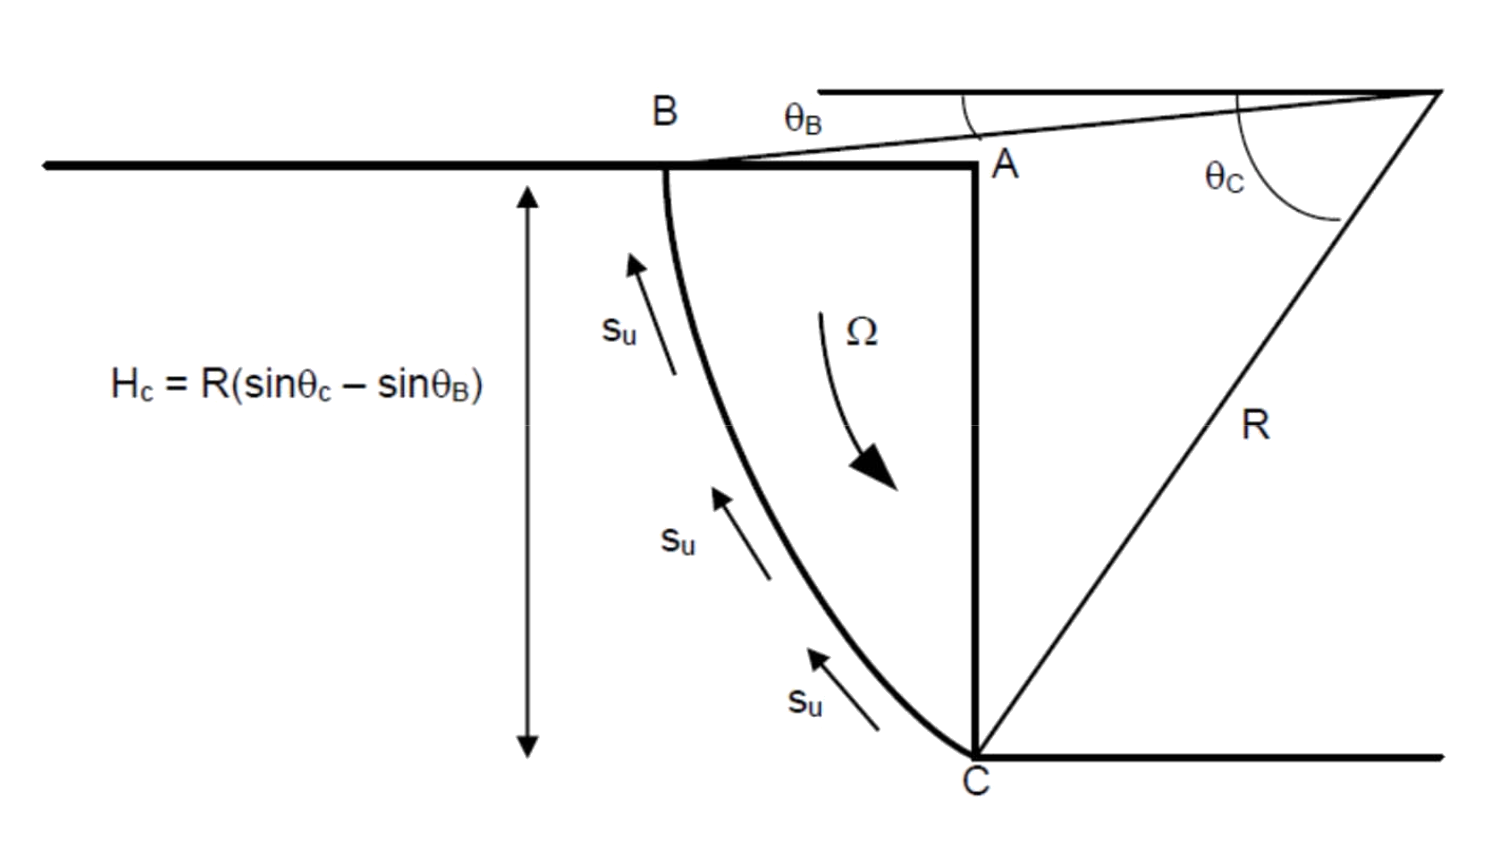
\includegraphics[width=0.6\linewidth]{figs/ub-cut-2.png}
	\end{figure}

	Change in potential energy of block ABC (Need to find the centroid and examine the
vertical movement by $\Omega$ = Dissipation = $s_u R (\theta_c - \theta_b) R \Omega$
	\begin{equation*}
	N_s = \frac{\gamma H_c}{s_u} = \frac{6 (\theta_c - \theta_b)}{2 \sin^2 \theta_c - \sin \theta_c \sin \theta_b - \sin^2\theta_b}
	\end{equation*}
	Optimizing: $\theta_b = 27.4^o$ and $\theta_c=57.5^o$. 
	$H_c = 3.83 s_u / \gamma$.
\end{frame}

\note{
Based on this solution: how far back from the edge of an unstable
vertical cut should you stand, to be safe if it fails?
These upper bounds are far from the lower bound calculated. With numerical methods, the lower bound can be improved,
and it is now accepted that the true solution is $\gamma H_c /s_u = 3.83$, to two significant figures, where the effective weight ($\gamma^\prime = \gamma - \gamma_w$) should be
used if the crack is water-filled.
}


%------------------------------------------------
\begin{frame}
	\frametitle{Taylor stability chart}
		\noindent
	\fboxsep=0pt
	\noindent
	\begin{minipage}[t]{0.5\linewidth}
		For sloped cuts as shown on the right, the critical height at different
slope
angles
($i$), different
		excavation depths ($H$) and
different rock depths ($n_d * H$) can
be evaluated using the following
		generalised formula.
		\begin{equation*}
			N_s = \frac{\gamma H_c}{s_u}		
		\end{equation*}
		where $N_s$ is the stability number
($N_s = 3.8$ for 90 degrees cut).
	\end{minipage}%
	\hfill
	\begin{minipage}[t]{0.5\linewidth}
	\begin{figure}
		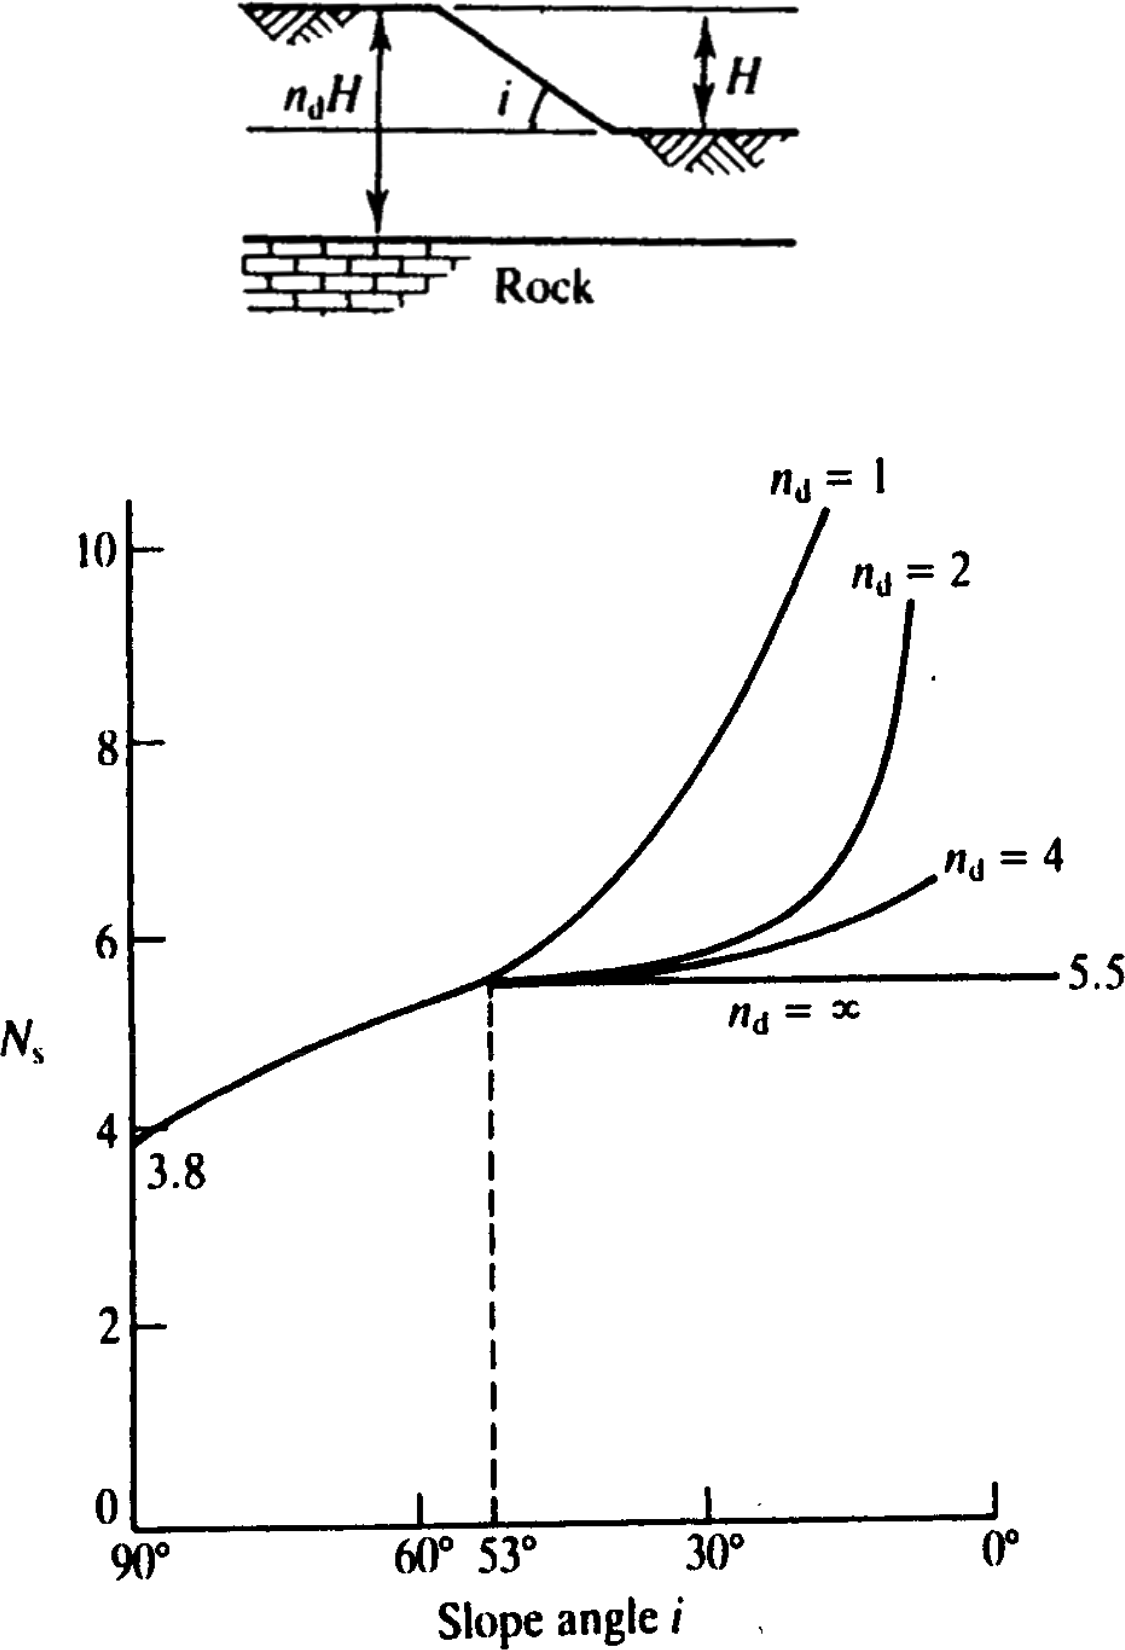
\includegraphics[width=0.85\linewidth]{figs/taylor-slope-stability.png}
	\end{figure}

	\end{minipage}

\end{frame}

%------------------------------------------------
\begin{frame}
 	\frametitle{Methods of analysis}
 	\mode<beamer>{
	\begin{table}[]
		\begin{tabular}{llllll}
			\toprule
			\textbf{Method of analysis} & \multicolumn{5}{c}{\textbf{Solution requirements}} \\
			\midrule
			& \rot{\textbf{Equilibrium}} & \rot{\textbf{Compatibility}} &
			\textbf{Constitutive law} &
			\rot{\textbf{Force}} & \rot{\textbf{Displacement}} \\
			\midrule
			\textbf{Closed form} & $\checkmark$ & $\checkmark$ & Linear elastic & $\checkmark$ & $\checkmark$ \\
			\textbf{Limit equilibrium} & $\checkmark$ &
			$\times$ & Rigid with a failure criterion & $\checkmark$ & $\times$ \\
			\textbf{Lower bound} & $\checkmark$ & $\times$ & Plasticity + flow-rule & $\checkmark$ & $\times$ \\
			\textbf{Upper bound} & $\times$ & $\checkmark$ & Plasticity + flow-rule & $\times$ & $\checkmark$ \\
			\textbf{Numerical analysis} & $\checkmark$ & $\checkmark$ & Any & $\checkmark$ & $\checkmark$ \\
			\bottomrule                        
		\end{tabular}
	\end{table}
	}
 	\mode<handout>{
	\begin{table}[]
		\begin{tabular}{llllll}
			\toprule
			\textbf{Method of analysis} & \multicolumn{5}{c}{\textbf{Solution requirements}} \\
			\midrule
			& \rot{\textbf{Equilibrium}} & \rot{\textbf{Compatibility}} &
			\textbf{Constitutive law} &
			\rot{\textbf{Force}} & \rot{\textbf{Displacement}} \\
			\midrule
			\textbf{Closed form} & & & Linear elastic & &  \\
			\textbf{Limit equilibrium} & & & Rigid with a failure criterion & & \\
			\textbf{Lower bound} &  &  & Plasticity + flow-rule &  & \\
			\textbf{Upper bound} & &  & Plasticity + flow-rule & &  \\
			\textbf{Numerical analysis} &  &  & Any &  &  \\
			\bottomrule                        
		\end{tabular}
	\end{table}
	}
\end{frame}
\end{document} 
